% !TeX program = xelatex
% !TeX encoding = UTF-8 Unicode
% !TeX spellcheck = en_EN-EnglishUnitedKingdom
% !TeX document-id = {6c471d8e-23aa-4982-9fb3-f8c46004c042}
\documentclass[12pt]{report}
\usepackage[backend=biber,refsection=chapter,style=ieee]{biblatex}
\usepackage{import}
\addbibresource{Chapter_3/ch3references.bib}
\addbibresource{Chapter_6/ch6references.bib}
\addbibresource{Chapter_7/ch7references.bib}
\addbibresource{Chapter_8/ch8references.bib}
% XeLaTeX
\usepackage{fontspec}
\setmainfont{Times New Roman}
% \setmonofont{Fira Code}
\setmonofont{PT Mono}
\usepackage{listings}
\usepackage{lstfiracode} % https://ctan.org/pkg/lstfiracode
\usepackage[margin=1in]{geometry}
\usepackage{setspace}
\usepackage{longtable}
\usepackage{supertabular}
\usepackage{afterpage}
\usepackage{lipsum}
\usepackage{circuitikz}
\usepackage{setspace}
\usepackage{listings}
\usepackage{xcolor}

% or LuaLaTeX
\def\BibTeX{{\rm B\kern-.05em{\sc i\kern-.025em b}\kern-.08em
    T\kern-.1667em\lower.7ex\hbox{E}\kern-.125emX}}

\sloppy
\setlength{\emergencystretch}{3em}
\raggedright

%\usepackage[sort]{natbib}
%\bibliographystyle{sb}
%    \bibpunct[:]{(}{)}{;}{a}{}{,}
\usepackage[colorlinks=false,hidelinks]{hyperref}  %change to true if you want to see links in color for drafting; hidelinks removes the boxes around links 

\ActivateVerbatimLigatures

%\usepackage{doi} % turns dois into links
\usepackage{gb4e}\noautomath %% or use expex, as preferred

\lstdefinestyle{python}{
    language=Python,
    basicstyle=\ttfamily\small,
    keywordstyle=\color{blue},
    stringstyle=\color{red},
    commentstyle=\color{gray},
    showstringspaces=false,
    frame=lines,
    numbers=left,
    numberstyle=\tiny\color{gray},
    breaklines=true
}

% Custom titles for the lists
\renewcommand{\lstlistlistingname}{List of Code Listings}

%%% Encoding and Fonts
\usepackage[english]{babel}
\usepackage{csquotes}
\usepackage{fontspec}
\usepackage{newtxtext}
\usepackage{xcolor}
\usepackage{listings}
\usepackage{microtype}
\usepackage{tabularx}
%\usepackage{mathastext}
%%% Page Layout and Spacing
\usepackage{geometry}
\geometry{a4paper, margin=1in}
\usepackage{parskip}
\parskip=0.5ex
\usepackage{setspace}
%%% Headers and Footers
\usepackage{fancyhdr}
\setlength{\headheight}{14.5pt}
\usepackage{lastpage}
\pagestyle{fancy}
\fancyhf{}
\fancyhead[R]{Page \thepage\ of \pageref{LastPage}}
\fancyfoot[R]{\leftmark: \rightmark}

%%% Math and Symbols
\usepackage{amsmath, amssymb, amsthm}

%%% Tables and Arrays
\usepackage{array, multirow, makecell, booktabs}
\renewcommand{\arraystretch}{1.3}
\usepackage{floatrow}
\DeclareFloatFont{Large}{\Large}
\floatsetup[table]{font=Large}

%%% Figures and Graphics
\usepackage{graphicx}
\graphicspath{{./images/}}
\DeclareGraphicsExtensions{.pdf,.png}
\usepackage{caption}
\usepackage{tikz}
\usepackage{circuitikz}
\usepackage{placeins}
\usepackage{pdfpages}
\usepackage{tcolorbox}

%%% Hyperlinks and References
\usepackage[hidelinks]{hyperref}
\usepackage{cleveref}

%%% Code Listings
\usepackage{pythonhighlight}
\usepackage{listings}
\usepackage{lstfiracode} % For Fira Code font style
\usepackage{fancyvrb}

\lstset{
    language=Python,
    style=FiraCodeStyle,
    basicstyle=\ttfamily\footnotesize,
    keywordstyle=\color{blue},
    stringstyle=\color{green!50!black},
    commentstyle=\color{gray},
    showstringspaces=false,
    breaklines=true,
    tabsize=4,
    numbers=left,
    numberstyle=\tiny\color{gray},
    frame=single,
    frameround=tttt,
    rulesepcolor=\color{black},
    postbreak=\mbox{\textcolor{red}{$\hookrightarrow$}\space}
}

%%% Typography and Lists
\usepackage{xcolor}
\definecolor{dgreen}{rgb}{0.,0.6,0.}
\definecolor{ochre}{cmyk}{0, .42, .83, .20}
\usepackage{enumitem}
\usepackage{url}
\usepackage[normalem]{ulem}
\usepackage{titlesec}
\usepackage{anyfontsize}
\usepackage{ragged2e}
\DeclareFloatFont{Large}{\Large}

\catcode"200B=9 % Ignore the zero-width space character

%%% Custom Commands
\newcommand\blankpage{%
    \null
    \thispagestyle{empty}%
    \addtocounter{page}{-1}%
    \newpage}

% Reference macros
\newcommand{\sref}[1]{\S\ref{#1}}
\newcommand{\srefs}[2]{\S\S\ref{#1}--\ref{#2}}
\newcommand{\eref}[1]{(\thechapter.\ref{#1})}
\newcommand{\erefs}[2]{\eref{#1}--\eref{#2}}
\newcommand{\earef}[2]{(\ref{#1}\ref{#2})}
\newcommand{\sbref}[1]{(\S\ref{#1})}
\newcommand{\reff}[1]{\hspace*{\fill}{\mbox{#1}}}
\newcommand{\refex}[2][]{\hfill\citep[#1]{#2}}
\newcommand{\reftex}[1]{\hspace*{\fill}\mbox{(#1)}}
\newcommand{\tref}[1]{Table~\ref{#1}\xspace}
\newcommand{\tpref}[1]{Table~\ref{#1} on page~\pageref{#1}\xspace}
\newcommand{\trefs}[2]{Tables~\ref{#1} and~\ref{#2}\xspace}
\newcommand{\fref}[1]{Figure~\ref{#1}\xspace}
\newcommand{\chref}[1]{Chapter~\ref{#1}\xspace}
\newcommand{\chrefs}[2]{Chapters~\ref{#1}--\ref{#2}\xspace}
\newcommand{\pref}[1]{page~\pageref{#1}\xspace}
\newcommand{\prefs}[2]{pages~\pageref{#1}--\pageref{#2}\xspace}
\newcommand{\aref}[1]{Appendix~\ref{#1}\xspace}
\newcommand{\qcite}[1]{\citeauthor{#1}'s (\citeyear{#1})\xspace}

% Text styling commands
\newcommand{\comm}[1]{\textsl{\textbf{\large{{#1}}}}}
\newcommand{\tit}[1]{\textit{{#1}}}
\newcommand{\tbf}[1]{\textbf{{#1}}}
\newcommand{\tsc}[1]{\textsc{{#1}}}
\newcommand{\fno}[1]{\footnote{\small #1}}
\newcommand{\nfno}[1]{\footnote{\tbf{#1}}}
\newcommand{\ul}[1]{\underline{{#1}}}
\renewcommand{\>}{\ensuremath >\xspace}
\newcommand{\<}{\ensuremath <\xspace}
\newcommand{\var}{\ensuremath{\sim}\xspace}
\newcommand{\eg}{e.g.\@\xspace}
\newcommand{\ie}{i.e.\@\xspace}
\newcommand{\nd}{n.d.\@\xspace}
\newcommand{\cf}{cf.\@\xspace}


\title{EE 322: EE Laboratory II \\
Final Portfolio}
\author{Steven Placzek}

\begin{document}

\thispagestyle{empty}
\begin{titlepage}
    \begin{center}
        \vspace*{0pt}
        \makeatletter    
        \Huge
        \textbf{\@title}\\
        \vspace{1ex}
        \Large
        \vspace{5ex}
        \textbf{\@author}\\
        \vfill
        \vspace{3ex}
        
\includegraphics[width=0.275\textwidth]{graphics/Seal_of_Western_New_England_University.png}\\
        \vspace{2ex}
        \large
        \textsc{Department of Electrical and Computer Engineering}\\
        \textsc{College of Engineering}\\
        \textsc{Western New England University}\\
        \vspace{.5cm}
        \normalsize \today
        \makeatother
    \end{center}

    \newpage

    \thispagestyle{empty}
    { }
\end{titlepage}

\chapter*{Abstract}
\thispagestyle{empty}
\emph{This portfolio documents a series of laboratory experiments conducted as part of EE322, with the objective of exploring and analyzing various MOSFET-based analog circuit topologies. The labs covered topics ranging from NMOS characterization and biasing techniques to the design and analysis of amplifiers and differential pairs. Experimental setups were implemented using the ALD1105/1106 transistor arrays and verified through simulations in LTSpice and Python-based data analysis. Circuit analyses techniques contained herein include the extraction of small-signal parameters, understanding the influence of source and load resistances on gain, and the role of feedback in stabilizing amplifier performance. Special emphasis was placed on evaluating frequency response, common-mode rejection, and the impact of grounding practices on measurement integrity. The final experiments introduced advanced concepts like S-parameter de-embedding using a Vector Network Analyzer (VNA), bridging analog design with RF characterization techniques. This comprehensive investigation demonstrates the critical interplay between theory, simulation, and practical implementation in analog circuit design.}


\pagenumbering{roman}



\addtocontents{toc}{\vspace{0pt}\protect\noindent\parbox[t]{\textwidth}{\normalsize\textcolor{black}{\textbf{Front matter}}}\par}


%\clearpage
%\phantomsection\addcontentsline{toc}{section}{Abstract}
%\stepcounter{page}

\singlespacing
\setstretch{0.95}
\tableofcontents
%\addcontentsline{toc}{section}{Table of contents}
\setstretch{1}

\listoffigures\addcontentsline{toc}{section}{List of Figures}
\listoftables\addcontentsline{toc}{section}{List of tables}

\normalsize
\newpage
\pagenumbering{arabic}
\doublespacing
\setlength{\parindent}{1.5em}
\chapter{Lab 1 — NMOS Characterization}
% !TeX root = main.tex

%\setkeys{Gin}{draft}
\onehalfspacing
\justifying
\par
This experiment aims to characterize an NMOS transistor for its relevant parameters, including threshold voltage ($V_{TH}$), transconductance parameter ($K$), and early voltage ($V_{A}$). The laboratory assignment utilizes Python to automate the measurement procedure and data acquisition. The ALD1106 is the device tested for this experiment.  

% Background Section
\section{Background}

Parameters $V_{TH}$, $K$, and $V_{A}$ are necessary parameters to determine both transistor bias points and small signal parameters. These parameters appear when examining the voltage-current characteristics of the NMOS transistor as follows:
\vspace{0.2cm}
\begin{itemize}
    \item \underline{Cutoff Mode:} $I_{D} = 0$ when $V_{GS} < V_{Tn}$ or $V_{DS}=0$
    
    \item \underline{Triode Mode:} $I_{D} = k_{n}^{'}\displaystyle \Bigg[\frac{W} {L}\Bigg]\Bigg(V_{OVn}-\frac{1}{2}V_{DS}\Bigg)V_{DS}$ when $V_{GS} > V_{Tn}$ \& $V_{DS}<V_{OVn}$
    
    \item \underline{Saturation Mode:} $I_{D} = K_{N}V_{OVn}^2\left(1+\displaystyle\frac{V_{DS}}{|V_{A}|}\right)$ when $V_{GS} > V_{Tn}$ \& $V_{DS}\geq V_{OVn}$ 
\end{itemize}
\vspace{0.2cm}
Typically in saturation mode, the $1+V_{DS}/|V_{A}|$ term is ignored when performing the DC analysis of a transistor circuit. However, in this lab experiment it is a critical parameter to ensure that the appropriate approximations can be made to linearize data for parameter extraction. 

\section{Experiment 1: \texorpdfstring{$I_{D}$ vs. $V_{DS}$}{ID vs. VDS}}
In this experiment, the $I_{D}$ vs. $V_{DS}$ curves will be generated by using the Rohde Schwarz NGU401 source measure unit (SMU) and the Keithley 3-channel programmable power supply. In this experiment, the SMU will simultaneously source the $V_{DS}$ voltage and measure the $I_{D}$ current in real time. The voltage $V_{GS}$ is generated by the programmable power supply as a family of curves is desired. A circuit schematic and wiring diagram are shown in Figure \ref{Ch1_fig:1}. The Python code list is under the Coding List in the Appendix. 
% \Cref{lst:Ch1List1}

\begin{figure}[ht]
    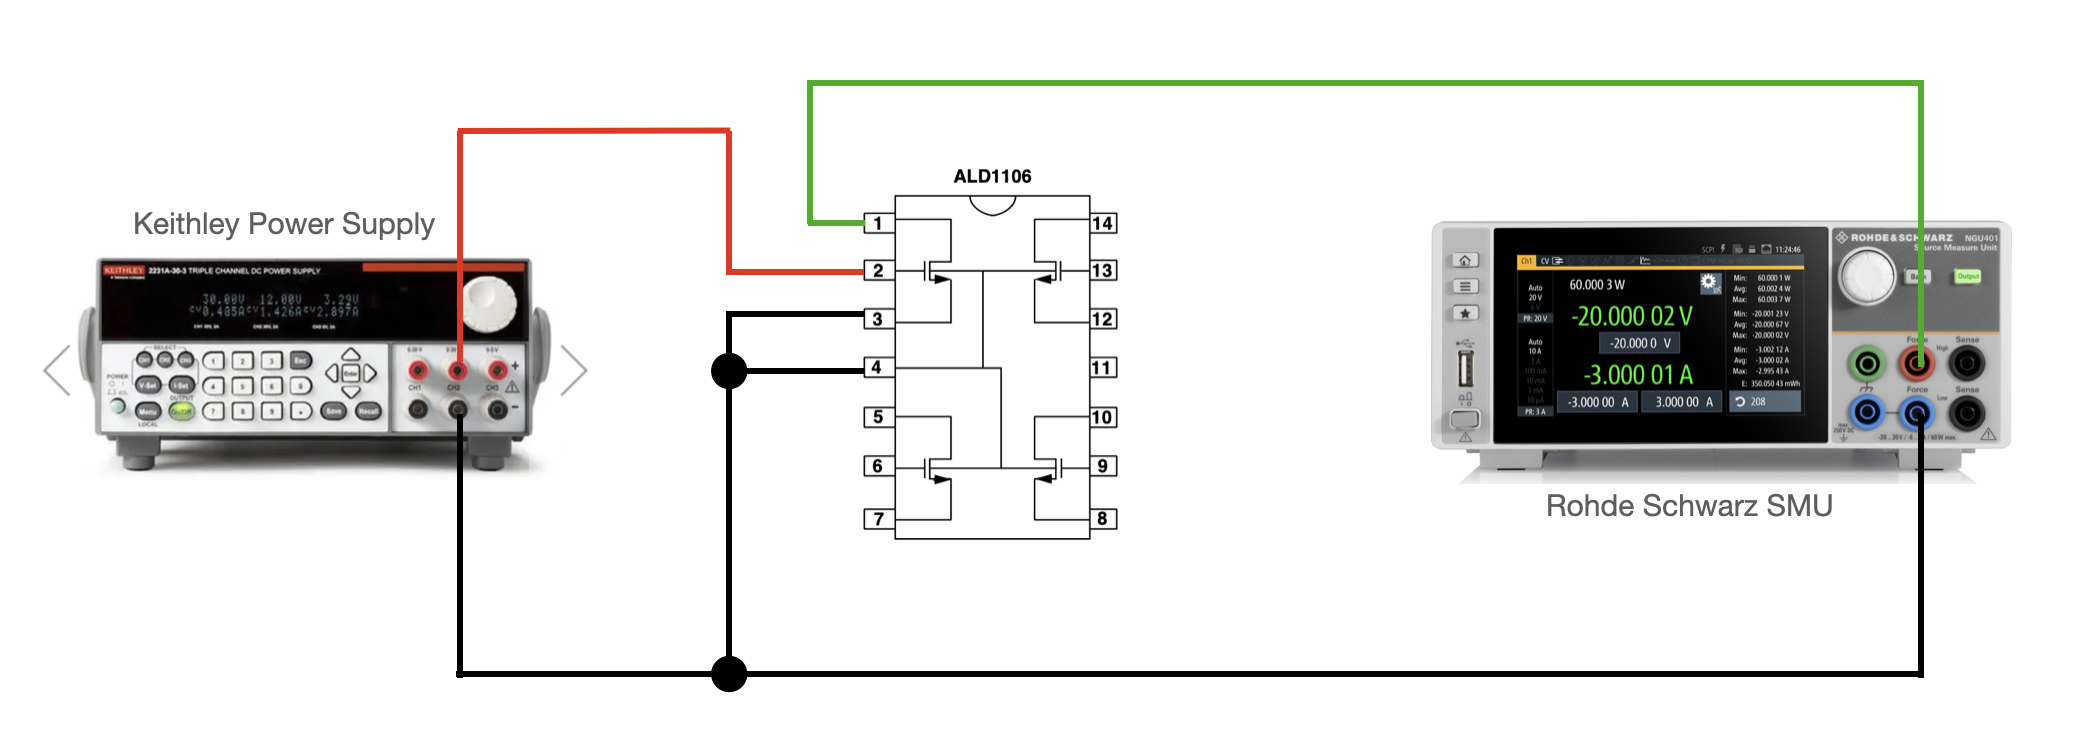
\includegraphics[scale=0.4]{graphics/Lab_01_1_1.png}
    \caption{Experiment 1 wiring diagram interfacing the transistor with the SMU and 3 channel power supply}
    \label{Ch1_fig:1}
\end{figure}

\section{Experiment 2: \texorpdfstring{$I_{D}$ vs. $V_{GS}$}{ID vs. VDS}}
In this experiment, the $I_{D}$ vs. $V_{GS}$ curves will be generated by using the Rohde Schwarz NGU401 source measure unit (SMU), the Keithley 3-channel programmable power supply and the Keithley digital multimeter (DMM). In this experiment, the SMU will source the $V_{GS}$ voltage. The voltage $V_{DS}$ is generated by the programmable power supply and the current $I_{D}$ is measured in real time by the Keithley DMM to generate the family of curves as desired. The circuit schematic remains the same; however, different voltages are being swept, therefore, the wiring diagram is modified as shown in Figure \ref{Ch1_fig:2}. The Python code list is under the Coding List~\Cref{lst:Ch1:List2}, in the Appendix. 

\begin{figure}[ht]
    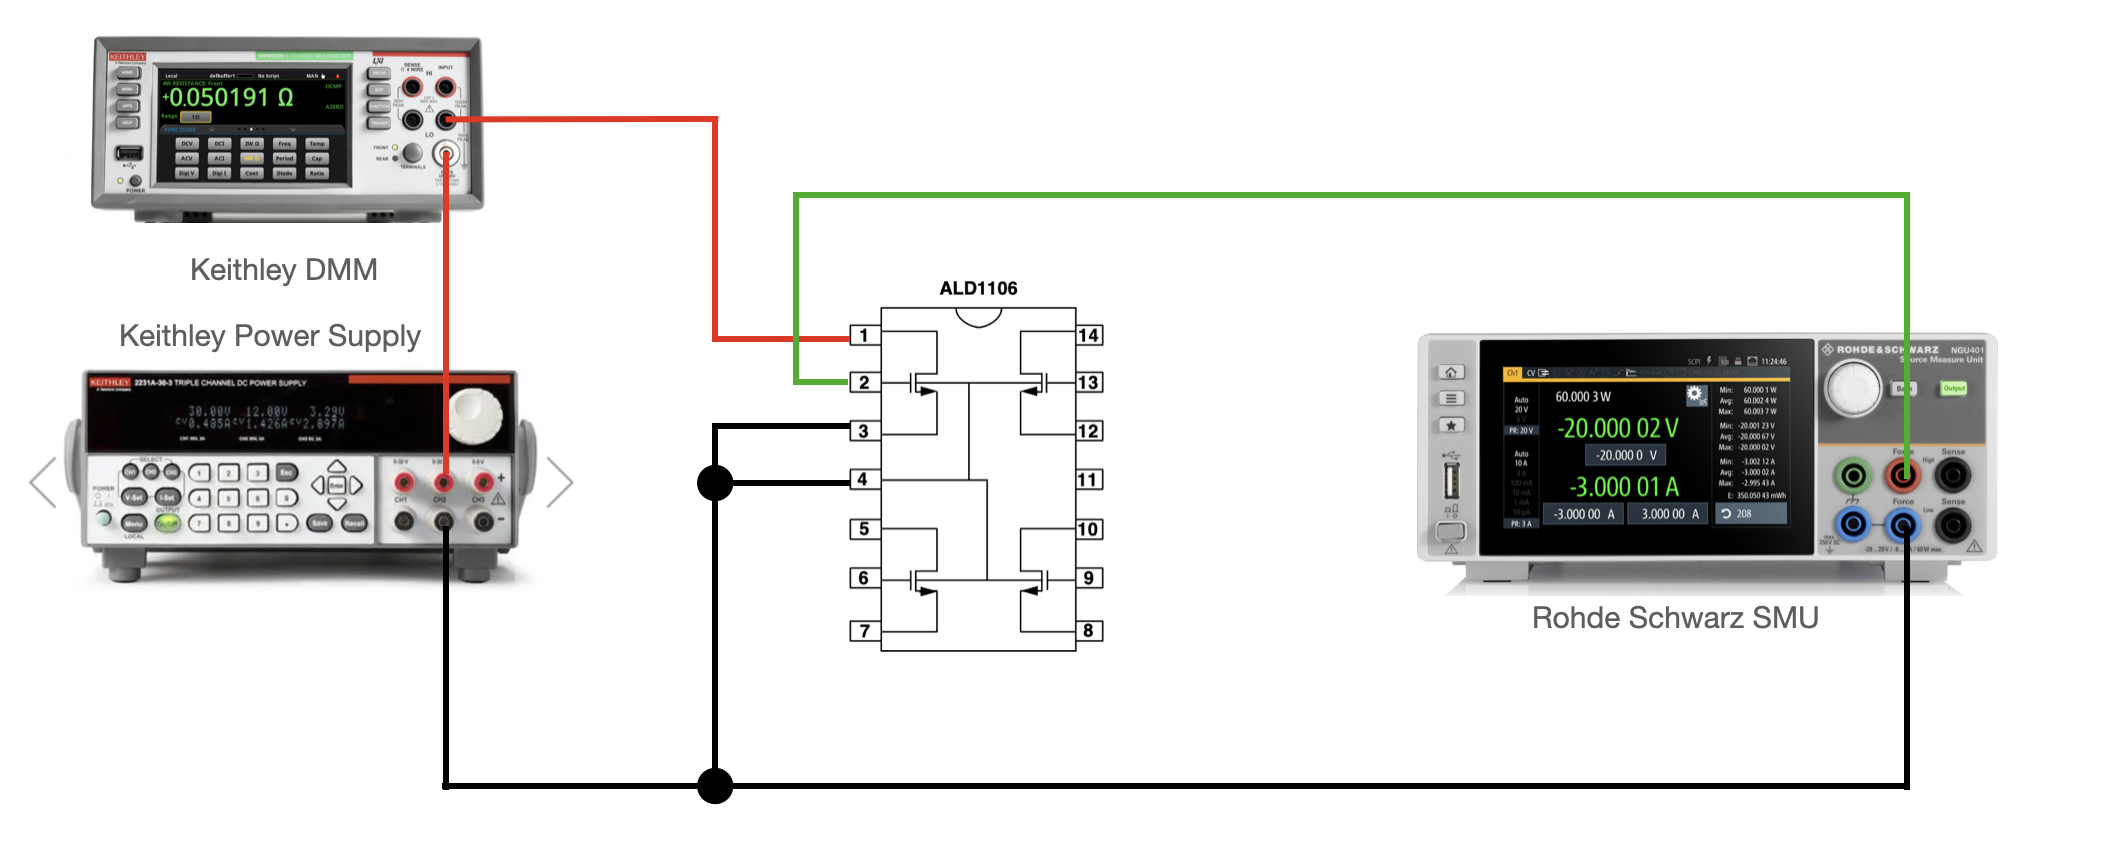
\includegraphics[scale=0.9\linewidth]{graphics/Lab_01_1_2.png}
    \caption{Experiment 2 wiring diagram interfacing the transistor with the SMU, 3 channel power supply, and digital multimeter}
    \label{Ch1_fig:2}
\end{figure}

\section{Results}
The post-laboratory tasks for this assignment included plotting the data from experiments 1 and 2. These plots include $I_{D}$ vs. $V_{DS}$ for a family of $V_{GS}$ values along with plotting $I_{D}$ vs. $V_{GS}$ for a family of $V_{DS}$ values. The transistor parameters $V_{TH}$, $K$, and $V_{A}$ are extracted by curving fitting the data from experiments 1 and 2. Code listing provides a detailed approach for the extraction of data parameters. Figure \ref{Ch1_fig:3} displays the summarized results of the experiments, and the data parameters are listed in Tables \ref{tab:1} and \ref{tab:2}.  
\cref{lst:Ch1:List3}


\begin{table}[ht]
    \centering
    \begin{tabular}{ | >{\centering\arraybackslash} m{3cm} | >{\centering\arraybackslash} m{3.5cm} |>{\centering\arraybackslash} m{5cm} | >{\centering\arraybackslash} m{2cm} | }
    \hline
    Quantity & Mean Value & Standard Deviation & Units \\
    \hline
    $K_{N}$ & 265.96 & 5.83 & $\mu$A/V \\
    \hline
    $V_{Tn}$ & 0.547 & 0.007 & V \\
    \hline

    \end{tabular}

    \caption{Summary of $\sqrt{I_{D}}$ vs. $V_{GS}$ extracted parameter values}

    \label{tab:1}
	
\end{table}

\begin{table}[ht]
\centering
\begin{tabular}{ | >{\centering\arraybackslash} m{5cm} |>{\centering\arraybackslash} m{4cm} | >{\centering\arraybackslash} m{2cm} | }
\hline
Quantity & Value & Units \\
\hline
$V_{A}$ $(V_{GS}=2$V) & -62.74 & V \\
\hline
$V_{A}$ $(V_{GS}=4$V) & -88.63 & V \\
\hline
$V_{A}$ $(V_{GS}=6$V) & -140.18 & V \\
\hline
\end{tabular}
\caption{Summary of $I_{D}$ vs. $V_{DS}$ extracted parameter values}
\label{tab:2}
\end{table}




\begin{figure}[ht]
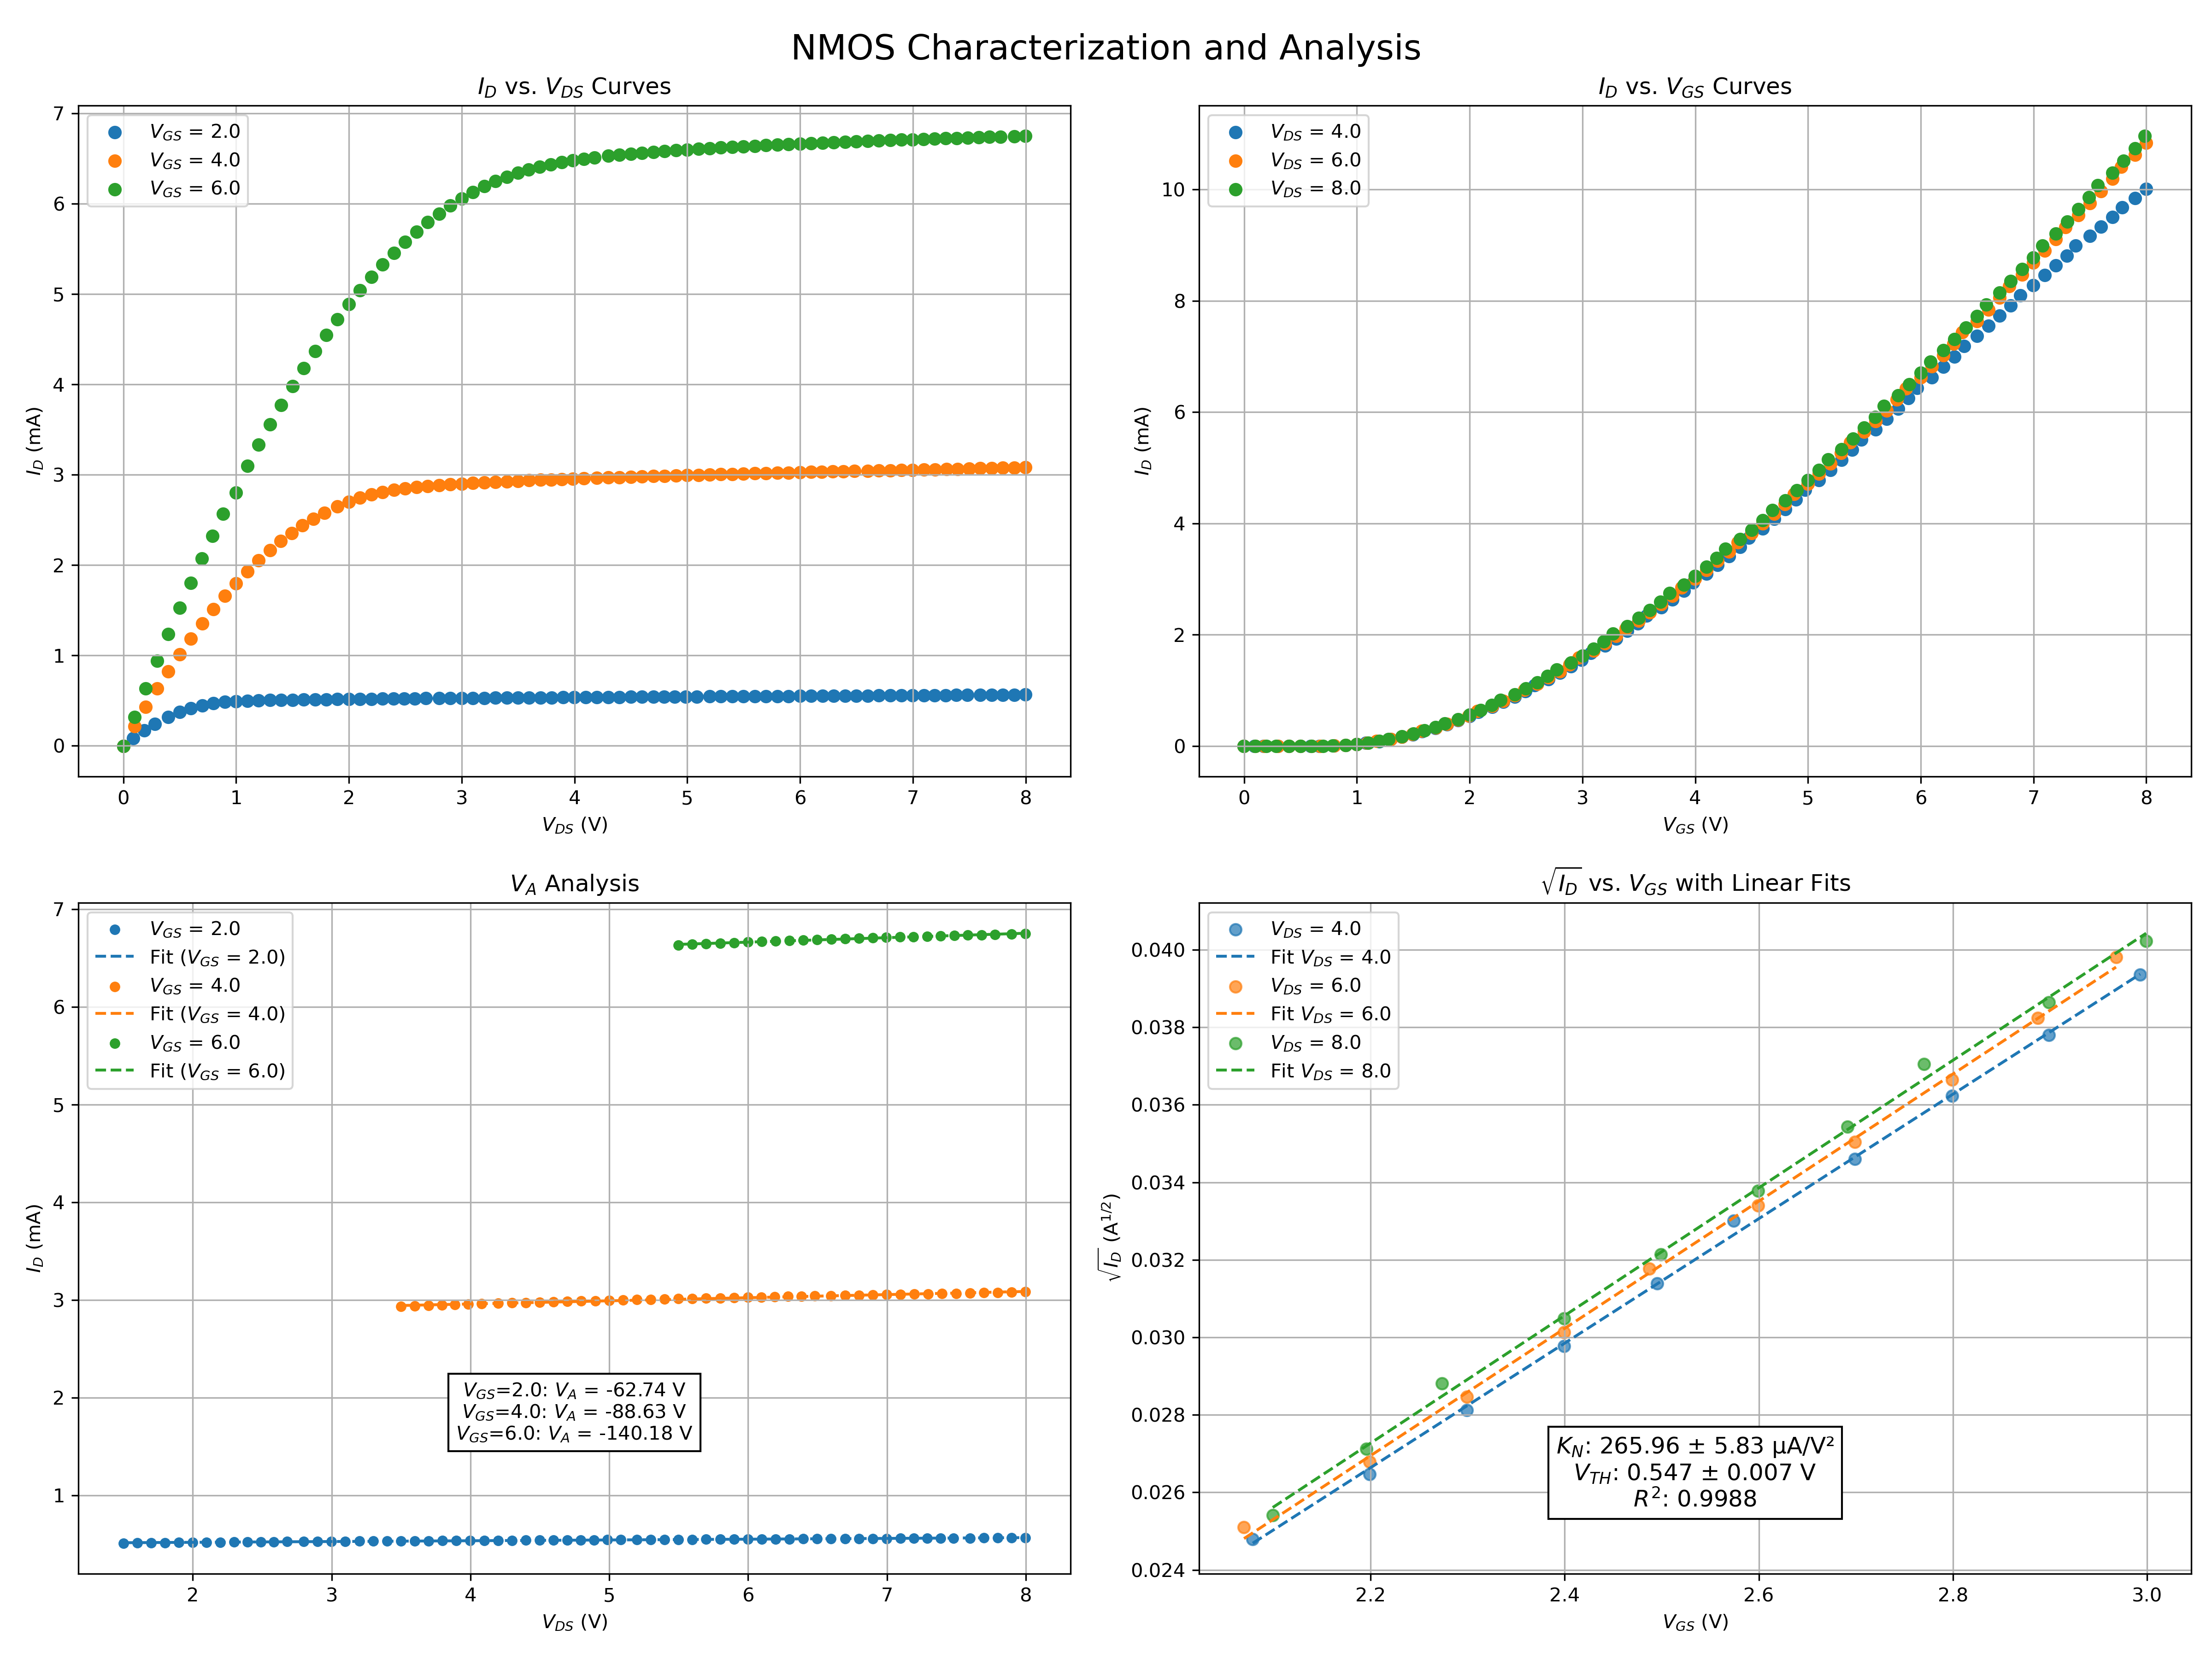
\includegraphics[scale=0.15]{graphics/Lab_01_1_3.png}
\caption{Summary of data for the NMOS characterization laboratory assignment}
\label{Ch1_fig:3}
\end{figure}

\section{Conclusions}
The data results indicate the NMOS transistor has a threshold voltage $V_{TH}$ = $0.547$, $K_{N}$ $=$ $265.96$ $\mu $ $A/V$, and Early voltages of $-62.75$, $-88.63$, and $-140.18$. The linearized region used to extract $V_{TH}$ \& $K_{N}$ had a coefficient of determination fit of $R^{2}$ $=$ $0.9988$ representing a near ideal fit across multiple data points with a small standard deviation among the various values of $V_{DS}$. The data points are chosen to minimize short channel effects from the measured results. In addition, it is experimentally observed that the Early voltage for each $V_{GS}$ sweep does not intersect the x-axis at the same point, indicating that the channel length modulation parameter is dependent on bias conditions. Therefore, when modeling this phenomenon, it likely requires a mathematical fit to fully caption its effects.
\chapter{Lab 2 — IC Biasing Techniques}
% !TeX root = main.tex

%\setkeys{Gin}{draft}

\onehalfspacing
\section{Lab Assignment Goals}
\justifying 

The goal of this lab was to study and compare the MOSFET-resistor biasing circuit and the beta multiplier circuit, specifically focusing on performance metrics such as power supply sensitivity. Biasing is essential in integrated circuits to establish proper operating points for transistors, ensuring consistent performance and linearity despite variations in temperature, power supply, or transistor parameters. The beta multiplier circuit is often preferred over a simple MOSFET-resistor configuration due to its ability to provide a more stable and predictable bias current, making it less sensitive to process and temperature variations. This stability is achieved through a feedback loop and multiple transistors that generate a reference current capable of adapting to changes, improving control and reliability in precision applications.  

To accomplish this, both circuits were simulated in LTSpice and built on a breadboard using the ALD1106/ALD1105 transistor array. Simulations and experimental measurements were conducted to analyze circuit behavior under different conditions, particularly variations in supply voltage. Data from both approaches were compared to evaluate the performance differences between the two biasing methods and to assess the advantages of the beta multiplier over the MOSFET-resistor configuration.

\begin{center}
\begin{figure}[ht]
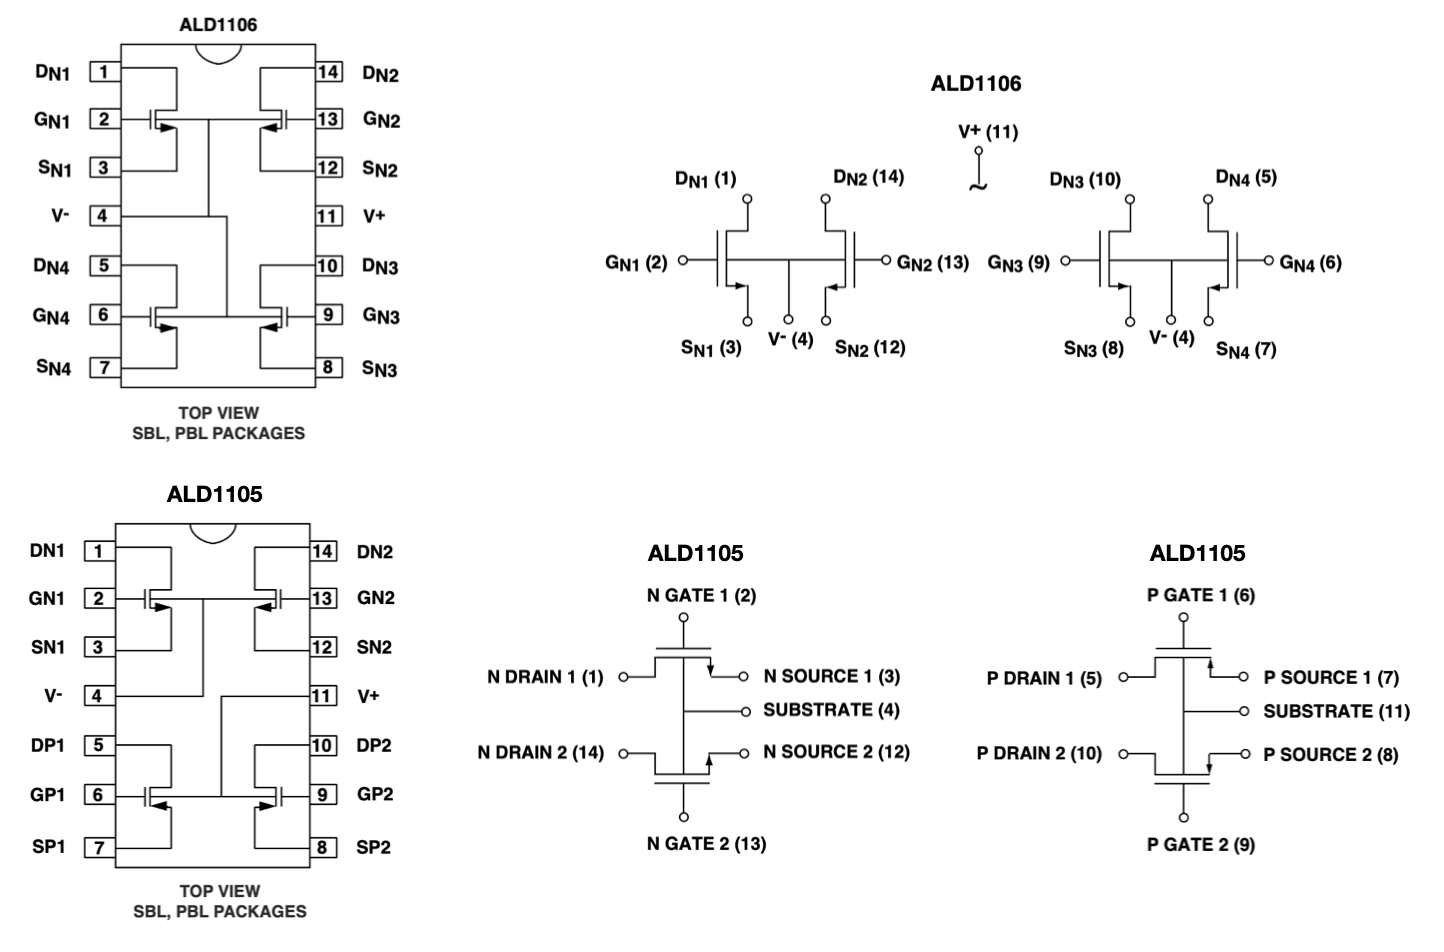
\includegraphics[scale=0.5\linewidth]{Chapter_2/Lab_02_Image_1.png}
\caption{The pinout and block diagram of the ALD1106 (top) and ALD1105 (bottom), \textbf{Note: $V^{-}$ is the body of the NMOS devices which is connected to lowest potential and $V^{+}$ is the body of the PMOS devices which is connected to the highest potential. }}
\label{fig:Ch2_fig1}
\end{figure}
\end{center}

\section{Experiment 1: The MOSFET-Resistor Characterization}

The objectives of this experiment involved characterizing a MOSFET-resistor circuit, as illustrated in the schematic below. The following tasks were performed:

\begin{itemize}
    
    \item The resistor was replaced with a 20k$\Omega$ potentiometer while setting $V_{DD} = 10$V. The resistance $R$ was determined at which $I_{D} = 500\mu$A.
    \item With the current set to $I_{D} = 500\mu$A, the DC operating point was identified.
    \item Finally, the supply voltage $V_{DD}$ was swept from 0 to 15V.
    
\end{itemize}

\begin{center}

\begin{circuitikz}[american]
\ctikzset{tripoles/mos style=arrows}

\draw

(0,0) node[nmos,scale=2] (Q1) {}
(Q1.center) node[right] {$Q_{1}$}
(Q1.S) node[ground] {} 
(Q1.D) to[R=$R$] ++(0,3) node[vcc] (vcc) {$+V_{DD}$}
(Q1.G) to[short] ++(-1,0) to[short] ++(0,1.5) to[short,-*] ++(2.96,0)

;   
\end{circuitikz}
\end{center}

\begin{center}
	\begin{figure}[ht]
	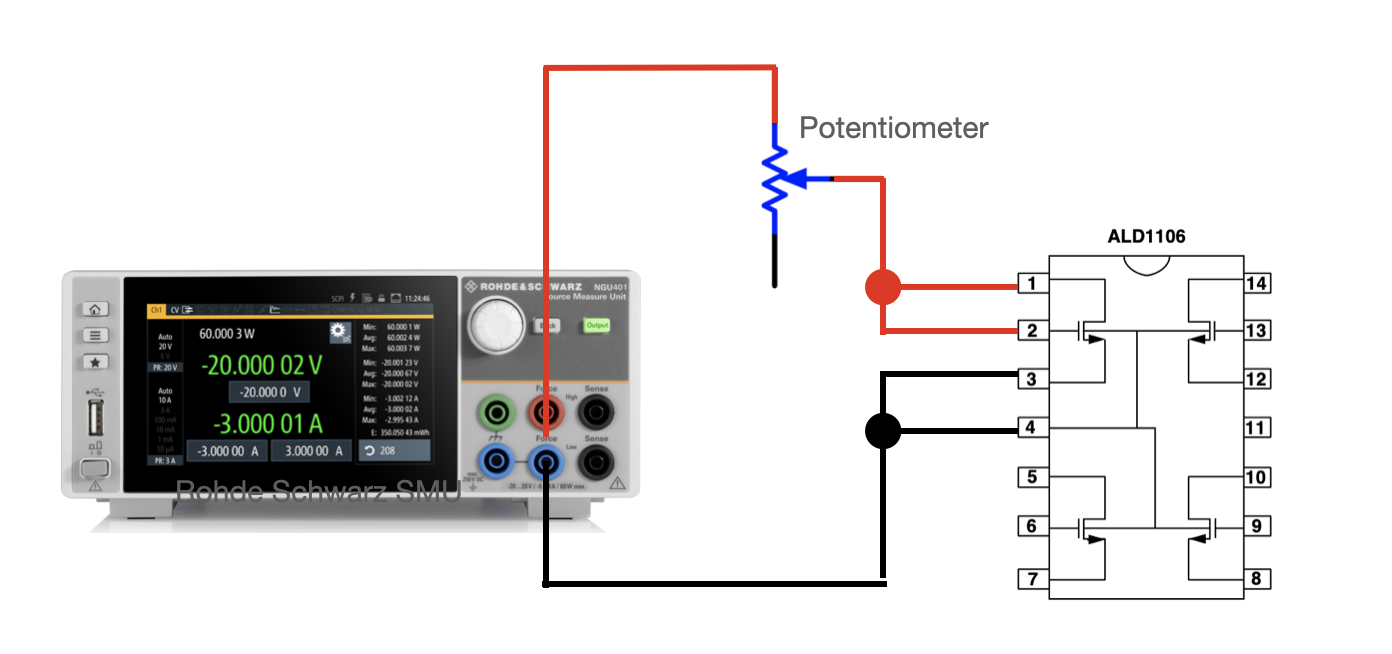
\includegraphics[scale=0.475\linewidth]{Chapter_2/Lab_02_Image_2.png}
	\caption{Wiring diagram of the MOSFET-resistor biasing circuit. The potentiometer had three terminals, with the top and bottom terminals used in combination with the middle terminal. }
	\label{Ch2_fig:2}
	\end{figure}
\end{center}

\newpage



%\newpage
\section{Experiment 2: The Beta Multiplier Characterization}

The objectives of this experiment involved characterizing a beta multiplier circuit, as illustrated in the schematic below. The following tasks were performed. Additionally, the width of $Q_{2}$ was four times that of $Q_{1}$, achieved by wiring four NMOS devices in parallel as available on the ALD1106:

\begin{itemize}

    \item The resistor was replaced with a 5k$\Omega$ potentiometer while setting $V_{DD} = 10$V. The resistance $R$ was determined at which $I_{D2} = 500\mu$A.
    \item With the current set to $I_{D2} = 500\mu$A, the DC operating point was identified.
    \item Finally, the supply voltage $V_{DD}$ was swept from 0 to 15V.
    \item Python Code used for this experiment can be found under the code listings~\cref{Ch2:List1}, ~\cref{Ch2:List2}, \& ~\cref{Ch2:List3}
    
\end{itemize}

\begin{center}

\begin{circuitikz}[american]
\ctikzset{tripoles/mos style=arrows}

\draw

(3,2) node[pmos,scale=1.5] (Q4) {}
(3,-2) node[nmos,scale=1.5] (Q2) {}
(-3,2) node[pmos,scale=1.5,xscale=-1] (Q3) {}
(-3,-2) node[nmos,scale=1.5,xscale=-1] (Q1) {}
(Q4.S) node[vcc] (vcc) {$+V_{DD}$}
(Q3.S) node[vcc] (vcc) {$+V_{DD}$}
(Q4.G) -- (Q3.G)
(Q1.G) -- (Q2.G)
(Q1.D) -- (Q3.D)
(Q2.D) -- (Q4.D)
(Q1.S) node[ground] {}
(Q2.S) to[R=$R$] ++(0,-2) node[ground] {}
(Q1.D) to[short,*-] ++(2,0) to[short,-*] ++(0,-1.15)
(Q4.D) to[short,*-] ++(-2,0) to[short,-*] ++(0,1.15)
(Q1.center) node[left] {$Q_{1}$}
(Q3.center) node[left] {$Q_{3}$}
(Q2.center) node[right] {$Q_{2}$}
(Q4.center) node[right] {$Q_{4}$}

;   
\end{circuitikz}

\begin{figure}[ht]
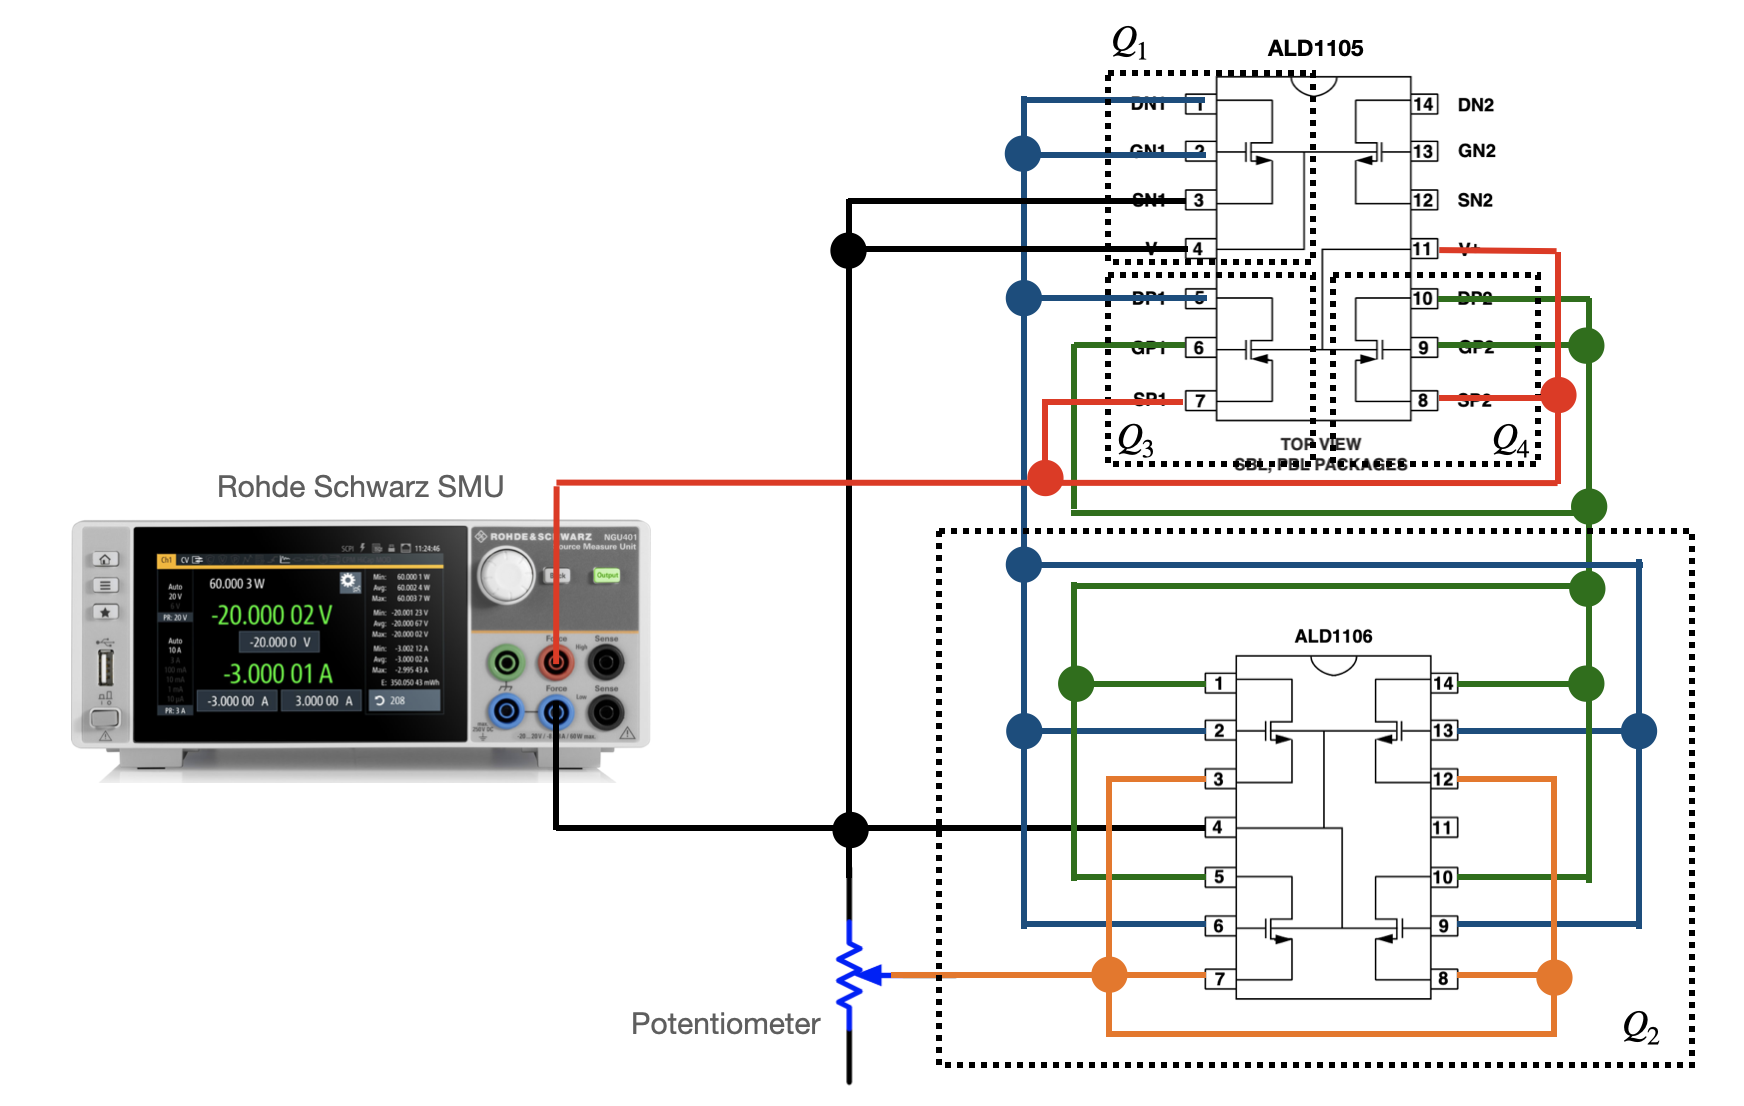
\includegraphics[scale=0.475\linewidth]{Chapter_2/Lab_02_Image_3.png}
\caption{Wiring diagram of the MOSFET-resistor biasing circuit. The potentiometer had three terminals, with the top and bottom terminals used in combination with the middle terminal. }
\label{Ch2_fig:2a}
\end{figure}

\end{center}

\newpage

\section{Post Lab Data Analysis}

The post-lab analysis involved the following tasks:

\begin{itemize}

    \item The circuits from Experiment 1 and Experiment 2 were simulated, following the same procedure of sweeping $R$ to determine the bias point at $I_{D} = I_{D2} = 500\mu$A. The DC operating point was then identified, followed by sweeping the power supply $V_{DD}$ from 0 to 15V.
    \item The tables for simulated and measured data were completed as specified.
    \item Both the simulated and measured power supply voltage sweeps were plotted on the same curve. The derivative of the simulated data was taken to determine the supply voltage sensitivity at the operating point $V_{DD} = 10$V.
    \item The results from Experiment 1 and Experiment 2 were compared to determine which circuit exhibited greater resistance to dynamic changes in the power supply.
    
\end{itemize}

\subsection{Experiment 1 - Results:}

\begin{center}
\begin{figure}[H]
	\centering
	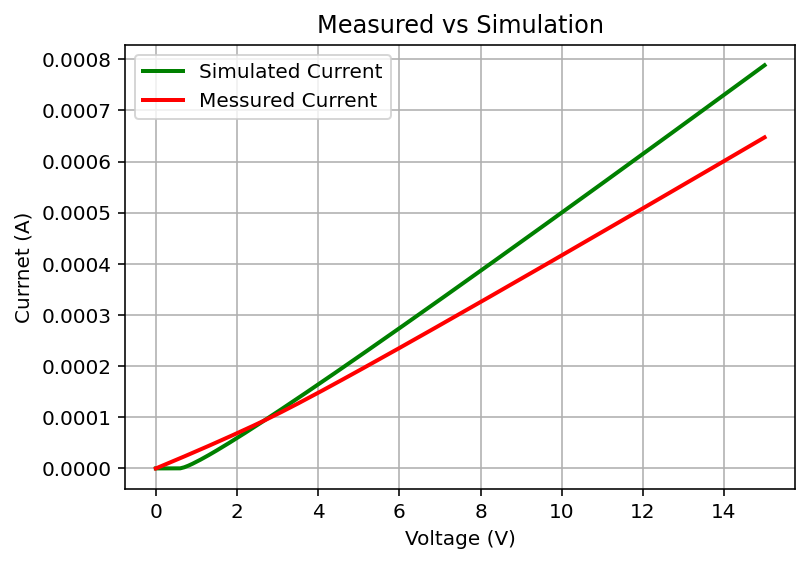
\includegraphics[width=0.65\linewidth]{Chapter_2/Lab_02_Exp_01_SIM_VS_MEAS_FINAL.png}
	\caption{Experiment 1: Simulated vs Measured Plot}
	\label{Ch2fig:1}
\end{figure}
\end{center}

\begin{center}
\begin{table}[H]
\begin{tabular}{| >{\centering\arraybackslash} m{3cm} | >{\centering\arraybackslash} m{3cm} | >{\centering\arraybackslash} m{3cm} | >{\centering\arraybackslash} m{2cm} |}
	\hline
	Quantity & Simulated & Measured & Units \\
	\hline
	$R$ & 16.200 & 16.003 & k$\Omega$ \\
	\hline
	$V_{GS1}$ & 1.91 & 1.940 & V \\
	\hline
	$V_{DS1}$ & 1.91 & 1.940 & V \\
	\hline
	$V_{OV1}$ & 1.337 & 1.341 & V \\
	\hline
	$I_{D1}$ & 499.999 & 504.477 & $\mu$A \\
	\hline
\end{tabular}
\caption{Experiment 1 Data Summary}
\end{table}
\end{center}

\newpage

\subsection{Experiment 2 - Simulated Results:}
The post-lab analysis involved comparing two circuit configurations, with the data clearly demonstrating that the circuit from Experiment 2 exhibits superior resistance to sudden changes in the power supply voltage. This enhanced stability can be attributed to the beta mirror configuration, which employs a cascade of current mirrors to maintain consistent current flow. The multiple transistor stages in the beta mirror create a high-impedance path that effectively isolates the bias current from power supply fluctuations. Additionally, the negative feedback inherent in the mirror configuration helps compensate for any variations in supply voltage by adjusting the gate-source voltages of the transistors to maintain constant current.
\vspace{0.25cm}

\begin{center}
	\begin{figure}
		\centering
		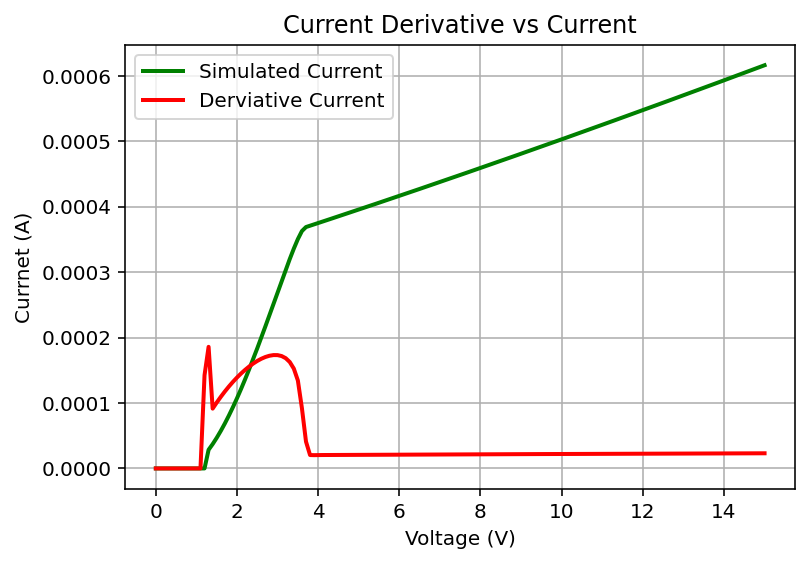
\includegraphics[scale=0.4]{Chapter_2/Lab_02_Exp_02_SIM_ID_vs_Derivative_Plot_FINAL.png}
		\caption{Experiment 2: Simulated $I_D$ vs $\frac{d}{dt}(I_D)$ Plot}
		\label{Ch2fig:2}
	\end{figure}
\end{center}

\begin{center}
\begin{table}[H]
\scriptsize
%	\renewcommand{\arraystretch}{1.4}
\setlength{\tabcolsep}{4pt} % default is 6pt
\begin{tabular}{| >{\centering\arraybackslash} m{3cm} | >{\centering\arraybackslash} m{3cm} | >{\centering\arraybackslash} m{3cm} | >{\centering\arraybackslash} m{2cm} |}
\hline
Quantity & Simulated & Measured & Units \\
\hline
$R$ & 1.254 & 1.0361 & k$\Omega$ \\
\hline
$V_{GS1}$ & 1.980 & 1.985 & V \\
\hline
$V_{DS1}$ & 1.980 & 1.985 & V \\
\hline
$V_{OV1}$ & 1.407 & 1.424 & V \\
\hline
$I_{D1}$ & 552.000 & 506.814 & $\mu$A \\
\hline
$V_{GS2}$ & 1.350 & 1.496 & V \\
\hline
$V_{DS2}$ & 6.420 & 6.646 & V \\
\hline
$V_{OV2}$ & 0.644 & 0.935 & V \\
\hline
$I_{D2}$ & 500.000 & 506.814 & $\mu$A \\
\hline
$V_{SG3}$ & 2.960 & 2.861 & V \\
\hline
$V_{SD3}$ & 8.020 & 8.006 & V \\
\hline
$|V_{OV3}|$ & 2.313 & 2.399 & V \\
\hline
$I_{D3}$ & 552.000 & 506.814 & $\mu$A \\
\hline
$V_{SG4}$ & 2.960 & 2.862 & V \\
\hline
$|V_{OV4}|$ & 2.313 & 2.301 & V \\
\hline
$I_{D4}$ & 500.000 & 506.814 & $\mu$A \\
\hline
\end{tabular}
\caption{Experiment 2 Data Summary}
\end{table}
\end{center}


\subsection{Experiment 2 - Simulated vs Measured Results:}

\begin{center}
	\begin{figure}[ht]
		\centering
		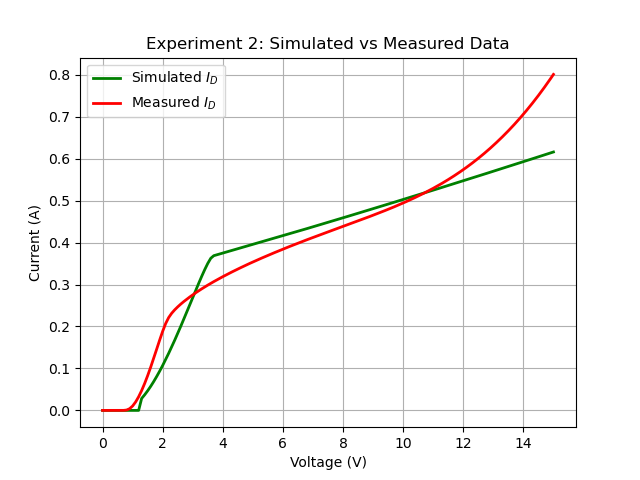
\includegraphics[scale=0.4]{Chapter_2/Lab_02_Exp_2_Sim_vs_Meas_Plot_FINAL.png} 
		\caption{Experiment 2: Simulated vs Measured Plots}
		\label{Ch2fig:3}
	\end{figure}
\end{center}

\section{Code Listings}

The Python implementations for the biasing analysis can be found in the Appendix: Plot Measured vs Simulated Data (\cref{lst:Ch2:List1}), Extract OP Values from LTSpice (\cref{lst:Ch2:List2}), Plot Measured vs Simulated Current (\cref{lst:Ch2:List3}), Calculate MOSFET Parameters (\cref{lst:Ch2:List4}), and Simulated vs Measured Data Plot (\cref{lst:Ch2List5}).

\section{Conclusion}
\justifying
This lab effectively demonstrated the differences in performance and robustness between a basic MOSFET-resistor biasing circuit and a beta multiplier biasing configuration. Through both simulation and physical prototyping, it was observed that while the MOSFET-resistor circuit can achieve the desired operating point with manual tuning, it suffers from significant sensitivity to changes in supply voltage. In contrast, the beta multiplier circuit consistently maintained a stable bias current across varying supply voltages, showcasing superior power supply rejection characteristics.

The enhanced stability of the beta multiplier can be attributed to its negative feedback mechanism and the use of matched transistor pairs, which allow the circuit to self-correct and adapt to fluctuations in external conditions. This makes it a preferred choice in precision analog and mixed-signal applications where stability and predictability are crucial.

Simulation results closely matched experimental data for both circuits, validating the modeling approach in LTSpice. Additionally, the derivative analysis confirmed that the beta multiplier exhibited a flatter response in current with respect to changes in $V_{DD}$​, quantitatively proving its reduced supply voltage sensitivity.

Overall, results highlight the importance of choosing appropriate biasing strategies in analog design and illustrated the trade-off between simplicity and performance in circuit design.


% \end{document}

\chapter{Lab 3 — Actively Loaded Common Source Amplifier}
% !TeX root = main.tex

%\setkeys{Gin}{draft}

\onehalfspacing
\section{Lab Assignment Goals}
\vspace{.35cm}
\justifying 

This objective of this lab assignment was to methodically evaluate a common source amplifier built with the ALD1105 MOSFET, with the overarching objective of determining how variations in load resistance and signal generator resistance affect circuit performance. The group’s tasks were organized into a series of experiments, each aimed at addressing distinct aspects of amplifier behavior.
In the first experiment, the DC operating point was established by adjusting the DC bias voltage $V_G$ until the output voltage $V_O$ reached $5$V. This step involved measuring node voltages and calculating the corresponding drain currents, providing a baseline for subsequent analysis. Establishing an accurate operating point is critical to ensure that the MOSFET operates in the intended region, which is a fundamental concept that can sometimes be overlooked in traditional electrical engineering coursework.
This experiment was intended to highlight the impact of how very slight adjustments to load resistance, along with signal generator resistance, will result in large changes with the output impedance and thus have a larger affect upon the overall stability of the circuit. 

\vspace{.35cm}

\begin{center}
\begin{figure}[ht]
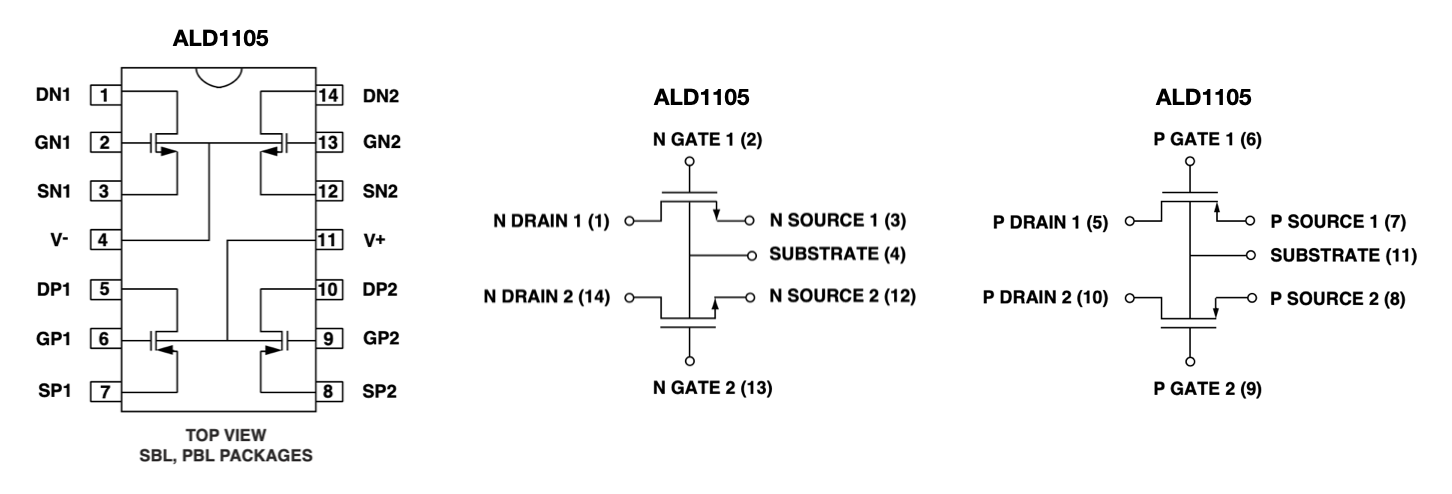
\includegraphics[scale=0.5\linewidth]{Chapter_3/Lab_03_Image_1.png}
\vspace{.55cm}
\caption{The pinout and block diagram of the ALD1105, \textbf{Note: $V^{-}$ is the body of the NMOS devices which is connected to lowest potential and $V^{+}$ is the body of the PMOS devices which is connected to the highest potential. }}
\label{Ch3_fig:1}
\end{figure}
\end{center}

\newpage

\section{Experiment 1: DC Operating Point}

Using the circuit shown below with the parameter values given, adjust the DC voltage $V_{GG}$ such that the output voltage $V_{O}$ = 5 V

\begin{itemize}

\item Find the dc operating point by measuring the node voltages and calculating the currents. Complete the summary table. 
	
\end{itemize}

\begin{center}
\begin{circuitikz}[american]
\ctikzset{tripoles/mos style=arrows}

\draw

(-4,2) node[pmos,scale=2,xscale=-1] (Q3) {}
(4,2) node[pmos,scale=2] (Q2) {}
(4,-3) node[nmos,scale=2] (Q1) {}
(Q3.center) node[left] {$Q_{3}$}
(Q2.center) node[right] {$Q_{2}$}
(Q1.center) node[right] {$Q_{1}$}
(Q3.S) node[vdd] (vdd) {$+V_{DD}$}
(Q3.D) to[R=$R$] ++(0,-3) node[ground] {}
(Q3.D) to[short,*-] ++(2.5,0) to[short,-*] ++(0,1.53)
(Q3.G) -- (Q2.G)
(Q2.S) node[vdd] (vdd) {$+V_{DD}$}
(Q1.S) node[ground] {}
(Q2.D) -- (Q1.D)
(Q1.G)  to[C=$C_{B}$] ++(-2,0) to[R=$R_{sig}$] ++(-2,0) to[vsource,l=$v_{sig}$] ++(0,-3) node[ground] {}
(Q1.G) to[R=$R_{G}$,*-] ++(0,2) node[vdd] (vdd) {$+V_{G}$}
(Q1.D) to[open] ++(0,1) node[left] {$V_{O}$}
(Q1.D) to[open] ++(0,1) to[C=$C_{B}$,*-] ++(3,0) to[R=$R_{L}$,v=$v_{o}$] ++(0,-3) node[ground] {}
;
\end{circuitikz}
\end{center}
\begin{center}
\vspace{1cm}
$V_{DD} = 10$ V \hspace{.5cm} $ V_{O} = 5$ V \hspace{.5cm} $C_{B} = 0.1 \mu$ F \\
\vspace{.2cm}
$R = 15$k $\Omega$  \hspace{.5cm} $R_{G} =10$M $\Omega$  \\
\vspace{.2cm}
$K_{N} = 270 \hspace{.25cm} \mu$A/V$^2$ \hspace{.25cm} $V_{T_n} = 0.573$ V \hspace{.25cm} $\lambda_{N} = 0.0165   $V$^{-1}$ \\
\vspace{.2cm}
$K_{P} = 88 \hspace{.15cm}  \mu$A/V$^2$ \hspace{.05cm} $V_{Tp} = -0.647$\hspace{.15cm}V \hspace{.25cm} $\lambda_{P} = 0.0219$  V$^{-1}$ \\
\vspace{.2cm}
\end{center}
\begin{center}
\begin{figure}[ht]
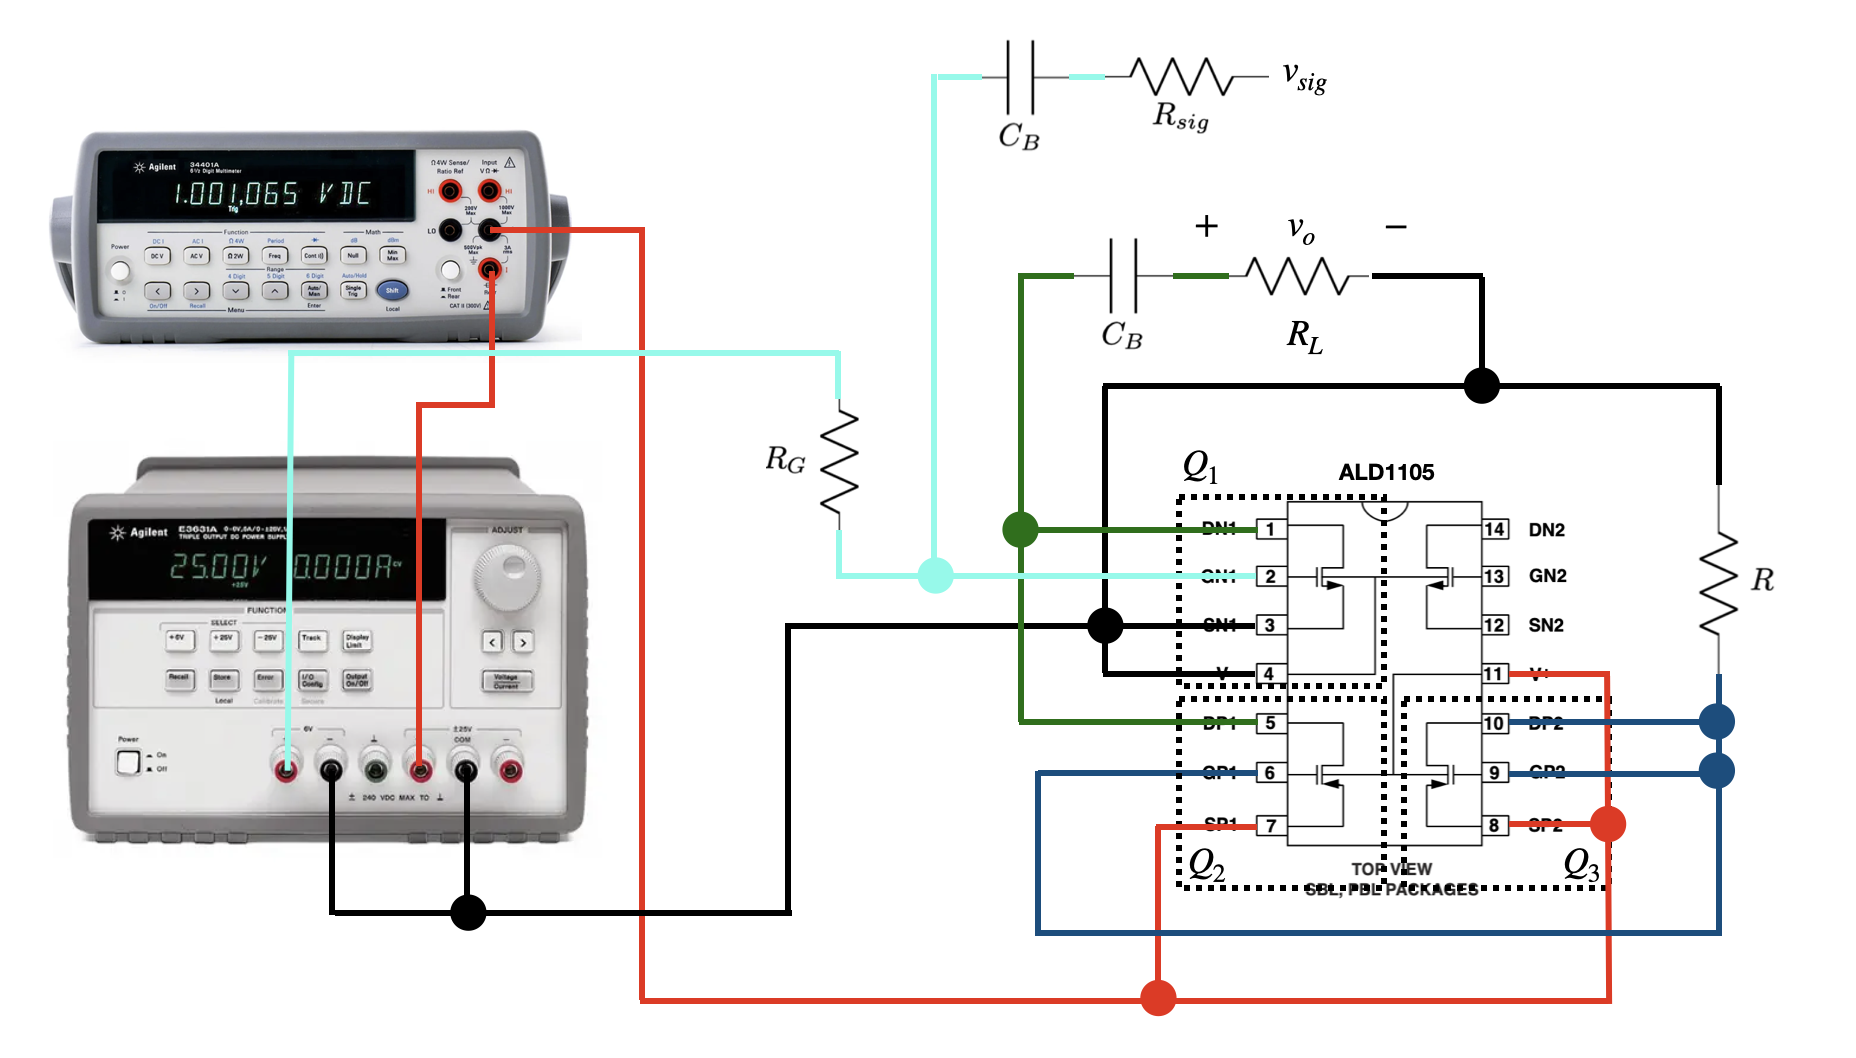
\includegraphics[scale=0.45]{Chapter_3/Lab_03_Image_2.png}
\caption{\emph{Wiring diagram of the Common Source Amplifier.}}
\label{Ch3_fig:2}
\end{figure}
\end{center}

\newpage

\vspace{.25cm}

\subsection{Measurement Issues \& 60 Hz Noise}

The physical measurement data were compromised due to improper grounding practices. In this instance, the use of separate ground rails resulted in ground loops that injected considerable $60$ Hz interference into the circuit measurements. This phenomenon is particularly problematic with the ALD1105 MOSFET, as its performance is highly sensitive to noise in the biasing network. Wiring the transistor to multiple different rails will result in ground loops that introduce significant $60$ Hz interference into measurement data, which this experiment demonstrated quite clearly. \cite{yao2015ecce}

In this scenario, the use of separate ground rails for the DC power supply, circuit, oscilloscope probes, and function generator led to mismatched ground potentials. According to an IEEE article on mitigating noise in electronic measurement systems, improper grounding practices can lead to the formation of ground loops that introduce significant $60 Hz$ interference into measurement data. In this case, using separate ground rails for the DC power supply, circuit, oscilloscope probes, and function generator resulted in mismatched ground potentials. This is particularly problematic when working with the ALD1105 MOSFET, which is highly sensitive to noise in its biasing network and operating conditions. \cite{cavache2023siitme}

\newpage
\section{Experiment 2: Investigating the Role of \texorpdfstring{$R_{sig}$}{Rsig}}

After establishing the DC operating point in Experiment 1, the role of the signal generator resistance, \(R_{sig}\), on the overall AC small-signal gain, \(G_v\), was investigated. The gain was defined as:

\[
G_v = \frac{v_o}{v_{sig}}
\]

The following procedure was implemented:

\begin{itemize}
    \item The load resistance was set to \(R_{L} = 10\,\text{M}\Omega\) (as provided by the oscilloscope probe).
    \item The small-signal gain, \(G_v\), was measured for various values of \(R_{sig}\), specifically for:
\end{itemize}
\vspace{0.2cm}
\begin{center}
\(R_{sig} = 10\,\text{M}\Omega\) \\[0.2cm]
\(R_{sig} = 100\,\text{k}\Omega\) \\[0.2cm]
\(R_{sig} = 10\,\text{k}\Omega\) \\[0.2cm]
\(R_{sig} = 1\,\text{k}\Omega\)
\end{center}


\section{Experiment 3: Investigating the Role of \texorpdfstring{$R_{L}$}{RL}}

Following the establishment of the DC operating point in Experiment 1, the influence of the load resistance, \(R_{L}\), on the AC small-signal gain, \(G_v\), was examined. The gain was defined as:

\[
G_v = \frac{v_o}{v_{sig}}
\]

The following procedure was executed:

\begin{itemize}
    \item The signal generator resistance was fixed at \(R_{sig} = 1\,\text{k}\Omega\).
    \item The small-signal gain, \(G_v\), was measured for various values of \(R_{L}\), specifically:
\end{itemize}
\vspace{0.2cm}
\begin{center}
\(R_{L} = 10\,\text{M}\Omega\) \\[0.2cm]
\(R_{L} = 100\,\text{k}\Omega\) \\[0.2cm]
\(R_{L} = 10\,\text{k}\Omega\) \\[0.2cm]
\(R_{L} = 1\,\text{k}\Omega\)
\end{center}

\section{Post Lab Data Analysis}

The post-lab analysis consisted of the following tasks:

\begin{itemize}

\item Simulate the circuits from experiments 1, 2, and 3 following the same procedure of sweeping $V_{GG}$ to find the bias point where $V_{O} = 5$V for experiment 1. Then operating under the bias condition, perform an AC analysis to find the ac small signal gain $G_{V}$ under the various $R_{sig}$ and $R_{L}$ conditions specified in experiments 2 and 3. 
\item The completed simulated data been entered into the tables, (\emph{the missing measurements will completed before the next lab meeting}), as specified below:
	
\end{itemize}

\begin{center}
	\begin{table}[H]
	\centering
	\renewcommand{\arraystretch}{1.0}
	\begin{tabular}{ | >{\centering\arraybackslash} m{2.5cm} | >{\centering\arraybackslash} m{2.5cm} | >{\centering\arraybackslash} m{2.5cm} | >{\centering\arraybackslash} m{2.5cm} | >{\centering\arraybackslash} m{2.5cm} | }
	\hline
	\multicolumn{5}{|c|}{\textbf{Experiment 1 Summary Table}} \\ \hline
	\textbf{Device} & \textbf{Quantity} & \textbf{Simulated} &\textbf{Measured} & \textbf{Units} \\ \hline
		\multirow{5}{*}{\(Q_1\)} 
		& \(I_{D}\)    & \(494.0\)  & $485.000$ & $\mu$A \\ \cline{2-5}
		& \(|V_{OV}|\) & \(1.299\)  & $1.290$ & V  \\ \cline{2-5}
		& \(V_{G}\)    & \(1.872\)  & $1.860$ & V  \\ \cline{2-5}
		& \(V_{D}\)    & \(5.058\)  & $4.970$ & V  \\ \cline{2-5}
		& \(V_{S}\)    & \(0.000\)  & $0.000$ & V  \\ \hline
		\multirow{5}{*}{\(Q_2\)}
		& \(I_{D}\)    & \(494.0\)  & $-480.000$ & $\mu$A \\ \cline{2-5}
		& \(|V_{OV}|\) & \(7.481\)  & $2.310$ & V \\ \cline{2-5}
		& \(V_{G}\)    & \(1.872\)  & $7.030$ & V \\ \cline{2-5}
		& \(V_{D}\)    & \(5.058\)  & $4.970$ & V \\ \cline{2-5}
		& \(V_{S}\)    & \(10.000\) & $9.990$ & V \\ \hline
		\multirow{5}{*}{\(Q_3\)}
		& \(I_{D}\)    & \(494.0\)  & $-480.009$ & $\mu$A \\ \cline{2-5}
		& \(|V_{OV}|\) & \(2.250\)  & $2.310$ & V \\ \cline{2-5}
		& \(V_{G}\)    & \(7.103\)  & $7.040$ & V \\ \cline{2-5}
		& \(V_{D}\)    & \(7.103\)  & $7.040$ & V \\ \cline{2-5}
		& \(V_{S}\)    & \(10.000\) & $9.99$ & V \\ \hline
	\end{tabular}
	\caption{Experiment 1 Summary Table}
	\end{table}
\end{center}

\newpage
\begin{center}
	\begin{table}[H]
	\renewcommand{\arraystretch}{1.2}
	\begin{tabular}{ | >{\centering\arraybackslash} m{3.5cm} | >{\centering\arraybackslash} m{2.5cm} | >{\centering\arraybackslash} m{2.5cm} | >{\centering\arraybackslash} m{2.5cm} | >{\centering\arraybackslash} m{2cm} | }
	\hline
	\multicolumn{5}{|c|}{\textbf{AC Small Signal Gain \(R_{L}=10\,\text{M} \Omega\)}} \\ \hline
	Condition & Quantity & Simulated  & Measured & Units \\ \hline
	\multirow{2}{*}{\(R_{sig}=10\,\text{M}\Omega\)} 
	 & \(G_{v}\)  & \(-21.900\)  & \(7.6110\)  & V/V   \\ \cline{2-5} 
	 & \(G_{v}\)  & \(26.810\)   & \(17.6288\)  & dB \\ \hline
	\multirow{2}{*}{\(R_{sig}=100\,\text{k}\Omega\)} 
	 & \(G_{v}\)  & \(-43.365\)  & \(16.2100\)  & V/V   \\ \cline{2-5} 
	 & \(G_{v}\)  & \(32.743\)   & \(24.1957\)  & dB \\ \hline
	\multirow{2}{*}{\(R_{sig}=10\,\text{k}\Omega\)} 
	 & \(G_{v}\)  & \(-43.756\)  & \(20.1700\)  & V/V   \\ \cline{2-5} 
	 & \(G_{v}\)  & \(32.821\)   & \(26.0941\)  & dB \\ \hline
	\multirow{2}{*}{\(R_{sig}=1\,\text{k}\Omega\)} 
	 & \(G_{v}\)  & \(-43.795\)  & \(22.3100\)  & V/V   \\ \cline{2-5} 
	 & \(G_{v}\)  & \(32.829\)   & \(26.9700\)  & dB \\ \hline
	\end{tabular}
	\caption{Experiment 2 Summary Table}
	\end{table}
\end{center}

\begin{figure}[H]
	\centering
	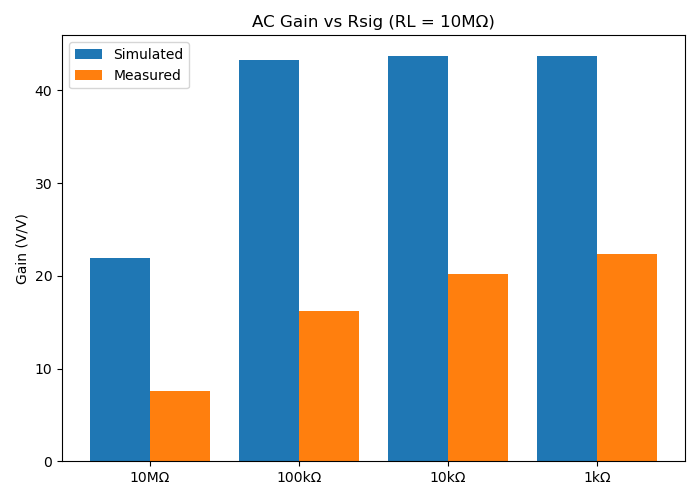
\includegraphics[width=0.75\linewidth]{Chapter_3/Lab_03_RL_10_Mohm.png}
	\caption{Simulated vs Measured data for $R_L = 10~\mathrm{M\Omega}$}
	\label{Ch3_fig:3}
\end{figure}

\newpage
\begin{center}
	\begin{table}[H]
	\centering
	\renewcommand{\arraystretch}{1.2}
		\begin{tabular}{ | >{\centering\arraybackslash} m{3.5cm} | >{\centering\arraybackslash} m{2.5cm} | >{\centering\arraybackslash} m{2.5cm} | >{\centering\arraybackslash} m{2.5cm} | >{\centering\arraybackslash} m{2cm} | }
		\hline
		\multicolumn{5}{|c|}{\textbf{AC Small Signal Gain \(R_{sig}=1\,\text{k} \Omega\)}} \\ \hline
		Condition & Quantity & Simulated  & Measured & Units \\ \hline
		\multirow{2}{*}{\(R_{L}=10\,\text{M}\Omega\)} 
		    & \(G_{v}\)  & \(-21.900\)  & \(31.2000\)  & V/V   \\ \cline{2-5} 
		    & \(G_{v}\)  & \(26.810\)   & \(20.881\)  & dB \\ \hline
		\multirow{2}{*}{\(R_{L}=100\,\text{k}\Omega\)} 
		    & \(G_{v}\)  & \(-13.943\)  & \(23.5000\)  & V/V   \\ \cline{2-5} 
		    & \(G_{v}\)  & \(22.887\)   & \(27.4214\)  & dB \\ \hline
		\multirow{2}{*}{\(R_{L}=10\,\text{k}\Omega\)} 
		    & \(G_{v}\)  & \(-3.240\)   & \(3.6500\)  & V/V   \\ \cline{2-5} 
		    & \(G_{v}\)  & \(10.211\)   & \(11.2459\)  & dB \\ \hline
		\multirow{2}{*}{\(R_{L}=1\,\text{k}\Omega\)} 
		    & \(G_{v}\)  & \(-0.373\)   & \(0.9510\)  & V/V   \\ \cline{2-5} 
		    & \(G_{v}\)  & \(-8.555\)   & \(-0.4364\)  & dB \\ \hline
		\end{tabular}
	\caption{Experiment 3 Summary Table}
	\end{table}	
\end{center}

\begin{figure}[H]
	\centering
	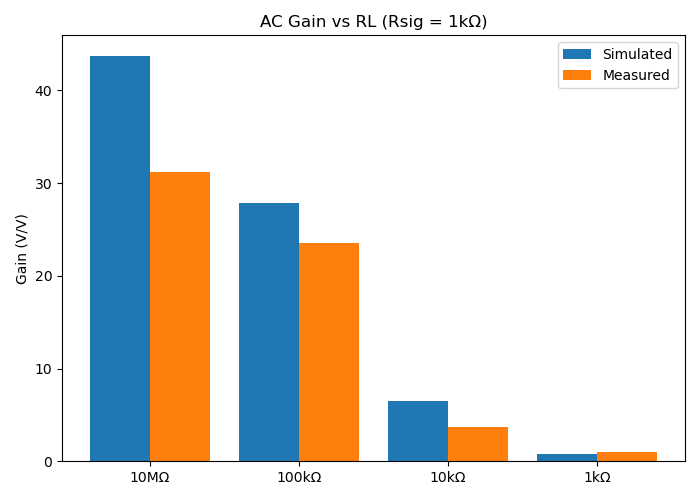
\includegraphics[width=0.75\linewidth]{Chapter_3/Lab_03_Rsig_1kohm.png}
	\caption{Simulated vs Measured data for $R_{\text{sig}} = 1~\mathrm{k\Omega}$}
	\label{Ch3_fig:4}
\end{figure}

\section{Code Listings}

The Python code used for the common source amplifier analysis can be found in the Appendix: Common Source Amp LTSpice Sweep (\cref{lst:Ch3:List1}).

\section{Conclusion}
\singlespacing
This lab successfully demonstrated the critical influence of source and load resistances on the performance of a common source amplifier using the ALD1105 MOSFET. Through a series of controlled experiments, both simulated and measured, the impact of varying $R_{sig}$​​ and $R_{L}$​​ on the AC small-signal gain $G_{V}$​ was thoroughly evaluated.

In Experiment 1, the DC operating point was accurately established by adjusting $V_{O}$​ such that the output voltage $V_{O}$ was $5$ V. This step confirmed the theoretical behavior of MOSFETs in the saturation region and emphasized the importance of correct biasing for reliable amplifier operation. The lack of close agreement between simulated and measured data reinforced the inaccuracy of the transistor model.

Experiment 2 showed that as $R_{sig}$​​ ​ decreased, the voltage gain $G_v$​ increased significantly, particularly in the measured results. This outcome is consistent with theoretical expectations, as a lower source resistance reduces signal attenuation before the gate of the MOSFET, allowing a greater portion of the input signal to modulate the channel current.
 
Experiment 3 revealed a strong dependence of gain on the load resistance $R_{L}$​​. Higher values of $R_{L}$​ led to markedly high gains, again matching theoretical predictions based on the amplifier’s gain formula $G_v \approx -g_m R_D \parallel R_L$​.  Results emphasized that loading effects from external measurement equipment (e.g., oscilloscope probes) or downstream circuitry can significantly influence observed performance.

The major insight from the lab was effects of grounding practices on measurement quality. Ground loops introduced substantial 60 Hz noise, initially preventing accurate gain readings. Once corrected, the improved grounding scheme allowed for reliable data collection that matched simulation trends closely. This lab demonstrated the sensitivity of analog circuits to parasitics and component values, especially in high-impedance configurations. Importance of thoughtful design and measurement practices is paramount for achieving predictable amplifier behavior.

\clearpage
\printbibliography[heading=subbibliography]
\chapter{Lab 4 — Frequency Response of the Common-Source Amplifier}
% !TeX root = main.tex

%\setkeys{Gin}{draft}
\onehalfspacing
\section{Lab Assignment Goals}
\vspace{0.25cm}
\justifying 
This lab involved implementing a common source amplifier using the ALD1105 MOSFET to analyze the frequency response. The primary objectives included measuring the DC operating point, such as the drain current and voltage, and generating a Bode plot of the frequency response. Since the internal capacitances of the MOSFETs were too small for the laboratory equipment to measure, discrete capacitors were added to mimic their behavior. These measurements provided insight into optimizing amplifier performance for various applications. LTSpice was used to validate measurement techniques. 

\begin{center}
\begin{figure}[ht]
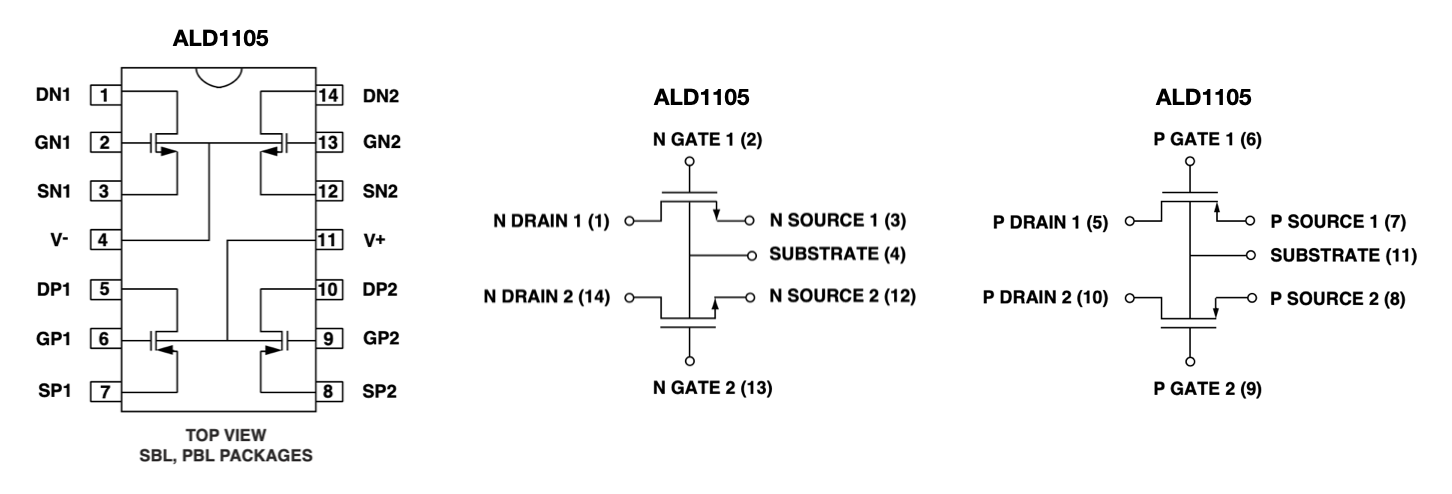
\includegraphics[scale=0.5]{Chapter_4/Lab_04_Image_1.png}
\caption{The pinout and block diagram of the ALD1105. \textbf{Note: $V^{-}$ is the body of the NMOS devices, which is connected to the lowest potential, and $V^{+}$ is the body of the PMOS devices, which is connected to the highest potential.}}
\label{Ch4_fig:1}
\end{figure}
\end{center}

\section{Experiment 1: DC Operating Point}

Using the circuit shown below with the given parameter values, the DC voltage $V_{GG}$ was adjusted such that the output voltage $V_{O}$ = $5$ V.

\begin{itemize}
    \item The DC operating point was determined by measuring the node voltages and calculating the currents. The summary table was then completed.
\end{itemize}

\begin{center}
\begin{circuitikz}[american]
\ctikzset{tripoles/mos style=arrows}
\draw

(-6,2) node[pmos,scale=2,xscale=-1] (Q3) {}
(4,2) node[pmos,scale=2] (Q2) {}
(4,-3) node[nmos,scale=2] (Q1) {}
(Q3.center) node[left] {$Q_{3}$}
(Q2.center) node[right] {$Q_{2}$}
(Q1.center) node[right] {$Q_{1}$}
(Q3.S) node[vdd] (vdd) {$+V_{DD}$}
(Q3.D) to[R=$R$] ++(0,-3) node[ground] {}
(Q3.D) to[short,*-] ++(2.5,0) to[short,-*] ++(0,1.53)
(Q3.G) -- (Q2.G)
(Q3.G) to[open,-*] ++(3,0) to[C=$C_{5}$] ++(0,2) node[ground,rotate=180] {}
(Q2.S) node[vdd] (vdd) {$+V_{DD}$}
(Q1.S) node[ground] {}
(Q2.D) -- (Q1.D)
(Q1.G)  to[short] ++(-2,0) to[C=$C_{B}$] ++(-2,0) to[R=$R_{sig}$] ++(-2,0) to[vsource,l=$v_{sig}$] ++(0,-3) node[ground] {}
(Q1.G) to[short] ++(-1.5,0) to[R=$R_{G}$,*-] ++(0,2) node[vdd] (vdd) {$+V_{G}$}
(Q1.G) to[short] ++(-1.5,0) to[C=$C_{1}$] ++(0,-2) node[ground] {}
(Q1.G) to[short] ++(-0.5,0) to[short,*-] ++(0,1.5) to[C,l=$C_{2}$,-*] ++(2.45,0)
(Q2.G) to[short] ++(-0.5,0) to[short,*-] ++(0,-1.5) to[C,l_=$C_{4}$,-*] ++(2.45,0)
(Q1.D) to[open] ++(0,1) node[left] {$V_{O}$}
(Q1.D) to[open] ++(0,1) to[C=$C_{B}$,*-] ++(3,0) to[R=$R_{L}$,v=$v_{o}$,*-] ++(0,-3) node[ground] {}
(Q1.D) to[open] ++(0,1) to[open] ++(3,0) to[short] ++(2,0) to[C=$C_{3}$] ++(0,-3) node[ground] {}
;
\end{circuitikz}
\end{center}

\section{Experiment 2: Frequency Response}

By employing appropriate AC measurement techniques, the frequency response of the amplifier was determined. The frequency range analyzed spanned from 10 Hz to 100 kHz. The following tasks were completed:

\begin{itemize}
    \item The mid-band gain $\left|G_{v\text{(mid)}}\right|$ was found.
    \item The bandwidth was determined by measuring $f_{L}$ and $f_{H}$, followed by computing the Gain Bandwidth Product (GBW) in Hz. The mid-band gain was converted to V/V.
    \item The measured and simulated results were plotted on the same curve, ensuring a magnitude range of 0 to +30 dB.
    \item The results for each experiment have been provided in the following tables.
    \item Calculations were done using Python and Simulations ran using LTSpice.
\end{itemize}

\newpage



\begin{center}

\begin{table}[H]
\begin{tabular}{ | >{\centering\arraybackslash} m{2.5cm} | >{\centering\arraybackslash} m{2.5cm} |  >{\centering\arraybackslash} m{2.5cm} | >{\centering\arraybackslash} m{2.5cm} | >{\centering\arraybackslash} m{2.5cm} |}
\hline
\multicolumn{5}{|c|}{DC Operating Point}        \\ \hline
                 Device & Quantity & Simulated  & Measured & Units \\ \hline
\multirow{5}{*}{$Q_{1}$} & $I_{D}$  & -485.30 & -492.70 & $\mu$A   \\ \cline{2-5} 
                  & $|V_{OV}|$ & 1.25 & 1.30 & V \\ \cline{2-5} 
                  &  $V_{G}$ & 1.85 & 1.85 & V  \\ \cline{2-5} 
                  & $V_{D}$ & 5.10 & 4.967 & V \\ \cline{2-5} 
                  & $V_{S}$ & 0.00 & 0.05 & V \\ \hline
                  &  &  &  &  \\ \hline
\multirow{5}{*}{$Q_{2}$} & $I_{D}$  & -473.564 & -492.70 & $\mu$A   \\ \cline{2-5} 
                  & $|V_{OV}|$ & 2.250 & 2.224 & V \\ \cline{2-5} 
                  &  $V_{G}$ & 7.103 & 7.129 & V  \\ \cline{2-5} 
                  & $V_{D}$ & 5.058 & 4.980 & V \\ \cline{2-5} 
                  & $V_{S}$ & 10.000 & 10.000 & V \\ \hline
                  &  &  &  &  \\ \hline
\multirow{5}{*}{$Q_{3}$} & $I_{D}$  & -473.564 & -473.600 & $\mu$A   \\ \cline{2-5} 
                  & $|V_{OV}|$ & 2.221 & 2.250 & V \\ \cline{2-5} 
                  &  $V_{G}$ & 7.120 & 7.100 & V  \\ \cline{2-5} 
                  & $V_{D}$ & 7.120 & 7.100 & V \\ \cline{2-5} 
                  & $V_{S}$ & 10.000 & 10.000 & V \\ \hline
\end{tabular}
\caption{DC Summary Table}
\end{table}

\begin{table}[H]
\begin{tabular}{ | >{\centering\arraybackslash} m{3.5cm} |  >{\centering\arraybackslash} m{3cm} | >{\centering\arraybackslash} m{3cm} | >{\centering\arraybackslash} m{2cm} |}
\hline
\multicolumn{4}{|c|}{AC Summary}        \\ \hline
                 Quantity & Simulated  & Measured & Units \\ \hline
$\left|G_{v\text{(mid)}}\right|$  & 27.325  & 17.361  & V/V   \\ \cline{1-4} 
$\left|G_{v\text{(mid)}}\right|$ & 28.731  & 24.791  & dB \\ \cline{1-4} \hline
 &  &  &  \\ \hline
$f_{L}$  & 44.668  & 101.604  & Hz   \\ \cline{1-4}
$f_{H}$ & 13.490  & 3.937  & kHz \\ \cline{1-4} \hline
 &  &  &  \\ \hline
$BW$  & 13.445  & 3.835  & kHz   \\ \cline{1-4}
$GBP$ & 367.384  & 66.582  & kHz \\ \cline{1-4} \hline
\end{tabular}
\caption{AC Summary Table}
\end{table}

\end{center}

%\clearpage
%\newpage

\section{Python Code Listings}

The Python implementation for frequency response analysis can be found in the Appendix (\cref{lst:Ch4:List1}).

\section{Conclusion}
\onecolumn
\justifying
\par
This lab focused on analyzing the frequency response of a common source amplifier by measuring its DC operating point, generating a Bode plot, and comparing simulated and measured data. Python code for this lab can be foud in the code listing \cref{Ch4:List1}. The process included adjusting the biasing conditions, sweeping the frequency response, and capturing key characteristics such as the lower and upper cutoff frequencies ($f_L$ and $f_H$), gain bandwidth product (GBP), and mid-band gain ($G_v$). The measured high-frequency cutoff ($f_H$) was found to be lower than the simulated value, indicating additional parasitic effects or variations in component behavior. The Miller Effect causes large discrepacies in the values between simulated and measured. The Miller effect states that if an impedance ($Z$) is in parallel with an inverting amplifier with a gain of magnitude $A$ (Figure 3, left), it can be split into two separate impedances at the input and output of the amplifier (Figure 3, right). 
The input and output impedances have values of $Z_{in} = \frac{1}{Z_1 + \frac{1}{A}}$ and $Z_{out} = \frac{Z_1}{1+A}$, respectively, and are both tied to ground.
\vspace*{0.10cm}
\par
Another critical factor is the \textbf{Miller effect}, which significantly impacts the high-frequency response of the amplifier. The Miller effect describes how the capacitance between the drain and gate ($C_{gd}$) is amplified by the voltage gain of the stage, effectively increasing the equivalent input capacitance. This phenomenon lowers the bandwidth by reducing the effective high-frequency cutoff. In simulations, SPICE models may not fully capture all secondary Miller capacitance effects, especially if they do not account for layout-dependent parasitics. In practical circuits, additional unintended capacitances and PCB trace effects further exacerbate the Miller effect, further decreasing the measured $f_H$ compared to the simulated value.
\vspace*{0.10cm}
\par
Results demonstrated how real-world variations influence circuit performance and emphasized the importance of simulation validation. Future work may involve refining the biasing network and improving frequency response accuracy through component selection and layout optimization.

\chapter{Lab 5 — Frequency Response of the Common Source Amplifier with Feedback}
% !TeX root = main.tex

%\setkeys{Gin}{draft}

\section{Assignment Goals}

%\onehalfspacing
\singlespacing
\justifying 
\par
In this lab, the common source amplifier from Lab 04 was modified by applying feedback to the circuit. Specifically, negative feedback was introduced by adding a resistor from the drain of $Q_{1}$ to the gate of $Q_{1}$. This feedback served multiple purposes, including stabilizing the DC bias point, eliminating the need for a dedicated bias voltage. The effect of feedback on bandwidth and gain was observed, showing an increase in bandwidth at the expense of overall circuit gain. However, it was also noted that feedback stabilized the gain, making it dependent only on the feedback resistor and, in this case, the signal generator resistor. The ALD1105 MOSFET was used to analyze the frequency response, and LTSpice simulations were conducted to validate measurement techniques.

\begin{center}
\begin{figure}[ht]
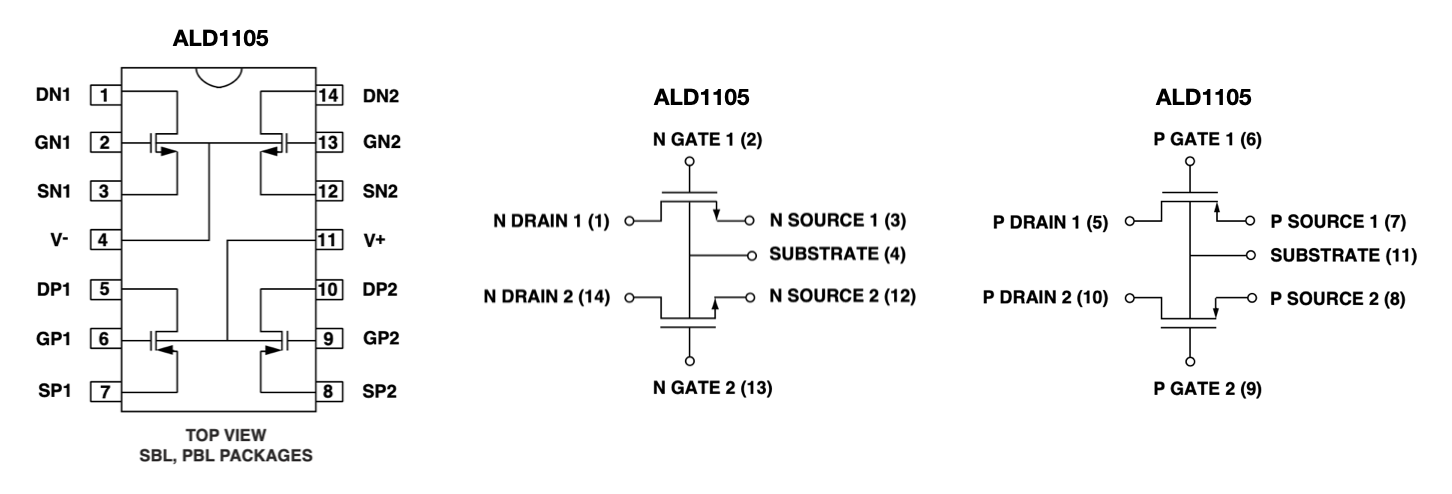
\includegraphics[scale=0.5]{Chapter_5/Lab_05_Image_1.png}
\caption{The pinout and block diagram of the ALD1105, \textbf{Note: $V^{-}$ is the body of the NMOS devices which is connected to lowest potential and $V^{+}$ is the body of the PMOS devices which is connected to the highest potential. }}
\label{fig:1}
\end{figure}
\end{center}

\section{Experiment 1: DC Operating Point}

Using the circuit shown below with the given parameter values, the potentiometer was adjusted to set the total current to $I_{Total} = 1$ mA.

\begin{itemize}

\item The DC operating point was determined by measuring the node voltages and calculating the currents. The summary table was then completed.

\end{itemize}

\begin{center}

\begin{circuitikz}[american]
\ctikzset{tripoles/mos style=arrows}

\draw

(-6,2) node[pmos,scale=2,xscale=-1] (Q3) {}
(4,2) node[pmos,scale=2] (Q2) {}
(4,-3) node[nmos,scale=2] (Q1) {}
(Q3.center) node[left] {$Q_{3}$}
(Q2.center) node[right] {$Q_{2}$}
(Q1.center) node[right] {$Q_{1}$}
(Q3.S) node[vdd] (vdd) {$+V_{DD}$}
(Q3.D) to[R=$R$] ++(0,-3) node[ground] {}
(Q3.D) to[short,*-] ++(2.5,0) to[short,-*] ++(0,1.53)
(Q3.G) -- (Q2.G)
(Q3.G) to[open,-*] ++(3,0) to[C=$C_{5}$] ++(0,2) node[ground,rotate=180] {}
(Q2.S) node[vdd] (vdd) {$+V_{DD}$}
(Q1.S) node[ground] {}
(Q2.D) -- (Q1.D)
(Q1.G)  to[short] ++(-2,0) to[C=$C_{B}$] ++(-2,0) to[R=$R_{sig}$] ++(-2,0) to[vsource,l=$v_{sig}$] ++(0,-3) node[ground] {}
(Q1.G) to[short,-*] ++(-1.5,0) to[short] ++(0,2.55) to[R=$R_{F}$] ++(3,0) to[short] ++(0.5,0) 
(Q1.G) to[short] ++(-1.5,0) to[C=$C_{1}$] ++(0,-2) node[ground] {}
(Q1.G) to[short] ++(-0.5,0) to[short,*-] ++(0,1.5) to[C,l_=$C_{2}$,-*] ++(2.45,0)
(Q2.G) to[short] ++(-0.5,0) to[short,*-] ++(0,-1.5) to[C,l=$C_{4}$,-*] ++(2.45,0)
(Q1.D) to[open] ++(0,1.5) node[left] {$V_{O}$}
(Q1.D) to[open] ++(0,1) to[C=$C_{B}$,*-] ++(3,0) to[R=$R_{L}$,v=$v_{o}$,*-] ++(0,-3) node[ground] {}
(Q1.D) to[open] ++(0,1) to[open] ++(3,0) to[short] ++(2,0) to[C=$C_{3}$] ++(0,-3) node[ground] {}
;
\end{circuitikz}

\vspace{1cm}

$V_{DD} = 10$ V \hspace{.5cm} $C_{B} = 0.022$ $\mu$F \hspace{.5cm}  $R = 25$ k$\Omega$ Potentiometer\\

\vspace{.2cm}

  $R_{F} =330$k $\Omega$ \hspace{0.5cm} $R_{sig} = 100$ k$\Omega$  \hspace{.5cm} $R_{L} =10$  M$\Omega$ (Probe)  \\

\vspace{.2cm}

$C_{1} = 10$ pF  \hspace{.5cm} $C_{2} =3.3$ pF \hspace{0.5cm} $C_{3} = 22$pF$+15$ pF (Probe)  \hspace{.5cm} $C_{4} =3.3$ pF \hspace{0.5cm} $C_{5} = 22$ pF  \\

\vspace{.5cm}
\end{center}

\section{Experiment 2: Frequency Response}
\singlespacing
Using appropriate AC measurement techniques, the frequency response of the amplifier was determined over a frequency range of 10 Hz to 100 kHz. Additionally, the following tasks were completed:

\begin{itemize}

\item The mid-band gain $\left|G_{v\text{(mid)}}\right|$ was measured.
\item The bandwidth was determined by measuring $f_{L}$ and $f_{H}$, and the Gain Bandwidth Product (GBW) was computed in Hertz. The mid-band gain was converted to V/V for accuracy.
\item The measured results were plotted against the simulated results on the same curve, using a magnitude range of 0 to +30 dB.
\item The summary tables at the end of the handout were completed.

\end{itemize}

\begin{center}


\begin{table}[H]
\begin{tabular}{ | >{\centering\arraybackslash} m{2.5cm} | >{\centering\arraybackslash} m{2.5cm} |  >{\centering\arraybackslash} m{2.5cm} | >{\centering\arraybackslash} m{2.5cm} | >{\centering\arraybackslash} m{2.5cm} |}
\hline
\multicolumn{5}{|c|}{DC Operating Point}        \\ \hline
                 Device & Quantity & Simulated  & Measured & Units \\ \hline
\multirow{5}{*}{$Q_{1}$} & $I_{D}$  & 525.197 & 500.290 & $\mu$A   \\ \cline{2-5} 
                  & $|V_{OV}|$ & 1.373 & 0.569 & V \\ \cline{2-5} 
                  &  $V_{G}$ & 1.945 & 1.142 & V  \\ \cline{2-5} 
                  & $V_{D}$ & 1.946 & 1.480 & V \\ \cline{2-5} 
                  & $V_{S}$ & 0.000 & 0.000 & V \\ \hline
                  &  &  &  &  \\ \hline
\multirow{5}{*}{$Q_{2}$} & $I_{D}$  & 525.197 & 500.290 & $\mu$A   \\ \cline{2-5} 
                  & $|V_{OV}|$ & 7.398 & 7.933 & V \\ \cline{2-5} 
                  &  $V_{G}$ & 1.956 & 1.142 & V  \\ \cline{2-5} 
                  & $V_{D}$ & 1.956 & 1.147 & V \\ \cline{2-5} 
                  & $V_{S}$ & 10.000 & 10.000 & V \\ \hline
                  &  &  &  &  \\ \hline
\multirow{5}{*}{$Q_{3}$} & $I_{D}$  & 474.798 & 500.290 & $\mu$A   \\ \cline{2-5} 
                  & $|V_{OV}|$ & 2.253 & 4.932 & V \\ \cline{2-5} 
                  &  $V_{G}$ & 7.100 & 4.421 & V  \\ \cline{2-5} 
                  & $V_{D}$ & 7.100 & 4.421 & V \\ \cline{2-5} 
                  & $V_{S}$ & 10.000 & 10.000 & V \\ \hline
\end{tabular}
\caption{DC Summary Table}
\end{table}

\newpage

\begin{table}[H]
\begin{tabular}{ | >{\centering\arraybackslash} m{3.5cm} |  >{\centering\arraybackslash} m{3cm} | >{\centering\arraybackslash} m{3cm} | >{\centering\arraybackslash} m{2cm} |}
\hline
\multicolumn{4}{|c|}{AC Summary}        \\ \hline
                 Quantity & Simulated  & Measured & Units \\ \hline
$\left|G_{v\text{(mid)}}\right|$  & 3.053  &  2.945 & V/V   \\ \cline{1-4} 
$\left|G_{v\text{(mid)}}\right|$ & 9.694  &  9.381 & dB \\ \cline{1-4} \hline
 &  &  &  \\ \hline
$f_{L}$  & 100.000 & 67.608 & Hz   \\ \cline{1-4}
$f_{H}$ & 63.100 & 138.038 & kHz \\ \cline{1-4} \hline
 &  &  &  \\ \hline
$BW$  & 137.971 & 137.971 & kHz   \\ \cline{1-4}
$GBP$ &  192.327 & 406.271 & kHz \\ \cline{1-4} \hline
\end{tabular}
\caption{AC Summary Table}
\end{table}

\end{center}

\newpage
\section{Measured Bode Plot}
\begin{center}
\begin{figure}[h]
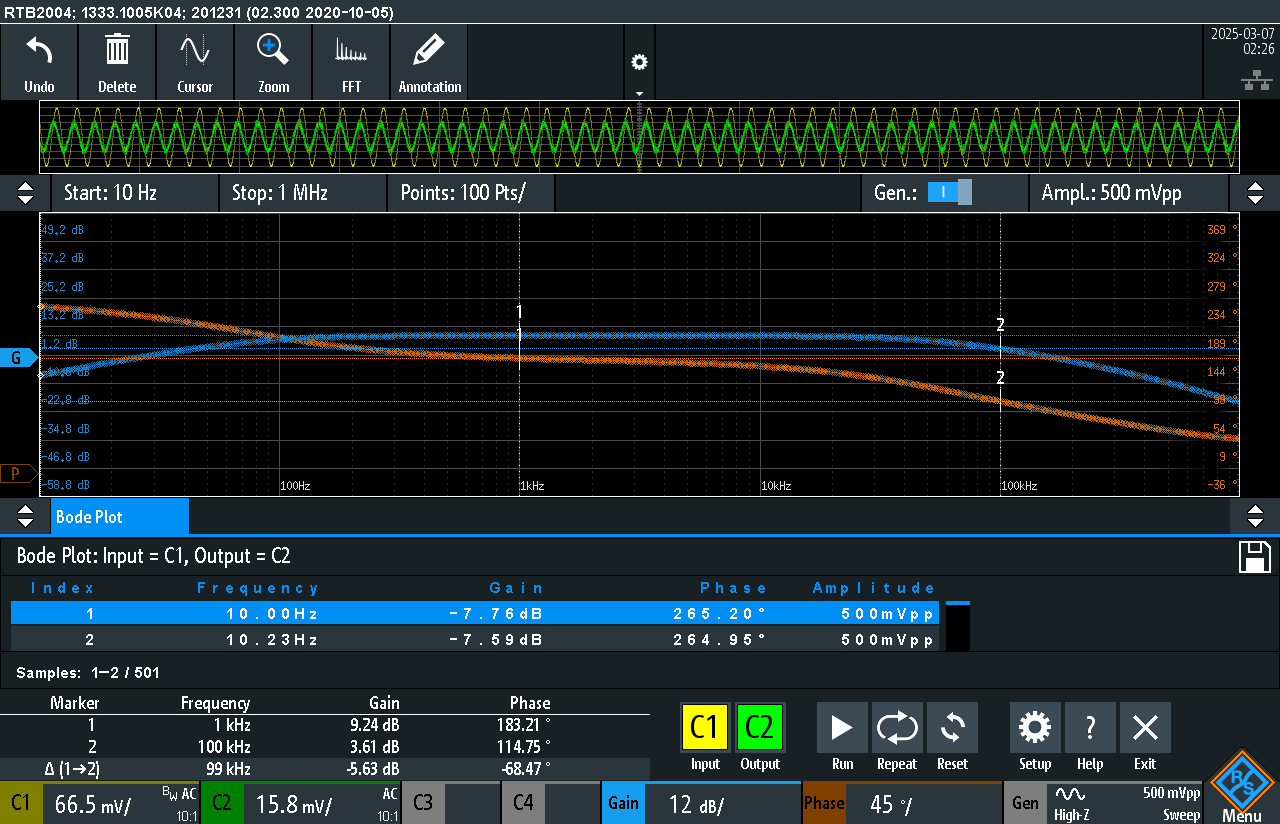
\includegraphics[scale=0.375]{Chapter_5/Lab05_Bode.png}
\caption{Measured Bode Plot of the Lab 05 circuit.}
\label{Ch5_fig:2}
\end{figure}
\end{center}

\section{Simulated vs Measured Plots}
\begin{figure}[H]
	\centering
	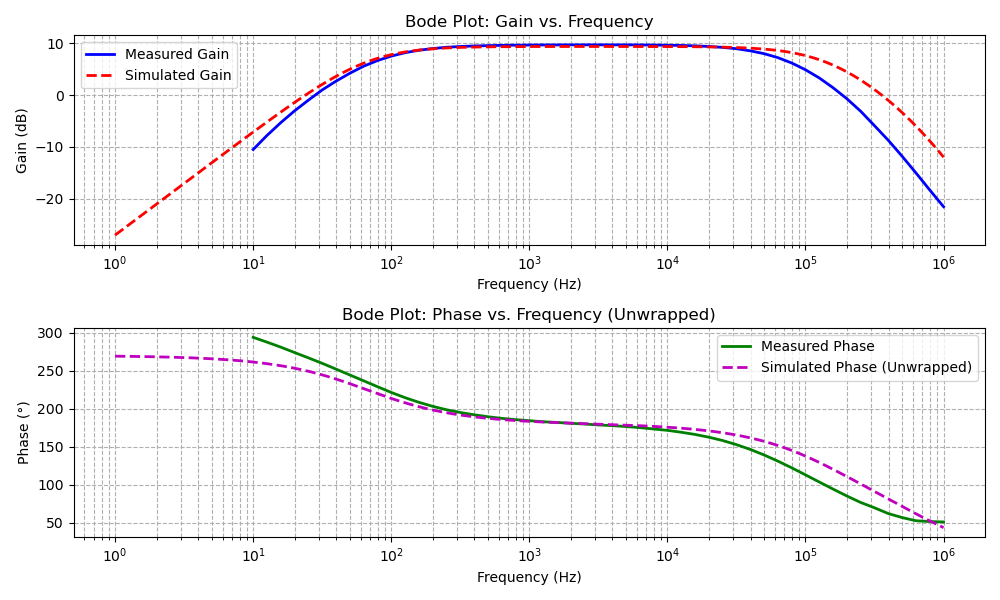
\includegraphics[width=1.0\linewidth]{Chapter_5/Lab_05_Bode_Sim_Vs_Meas_Gain_Phase.png}
	\caption{Simulated vs Measured Gain \& Phase}
	\label{Ch5_fig:3}
\end{figure}

\begin{figure}[H]
	\centering
	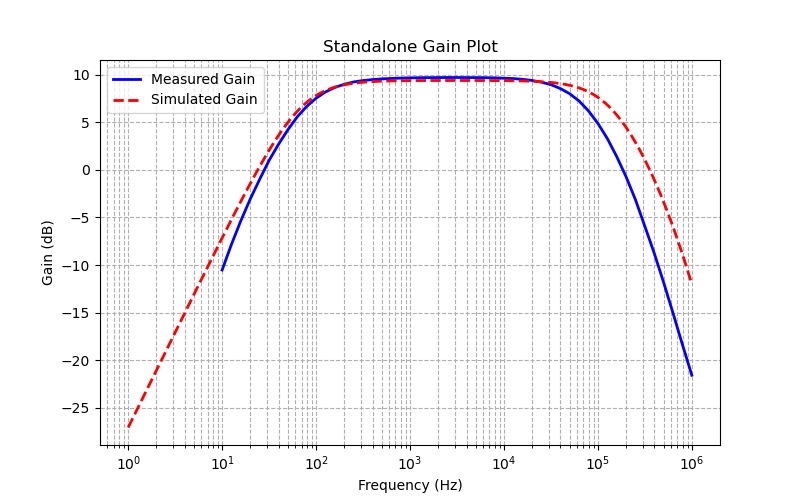
\includegraphics[width=1.0\linewidth]{Chapter_5/Lab_05_Sim_Vs_Meas_Gain.png}
	\caption{Simulated vs Measured Gain}
	\label{Ch5_fig:4}
\end{figure}

\begin{figure}[H]
	\centering
	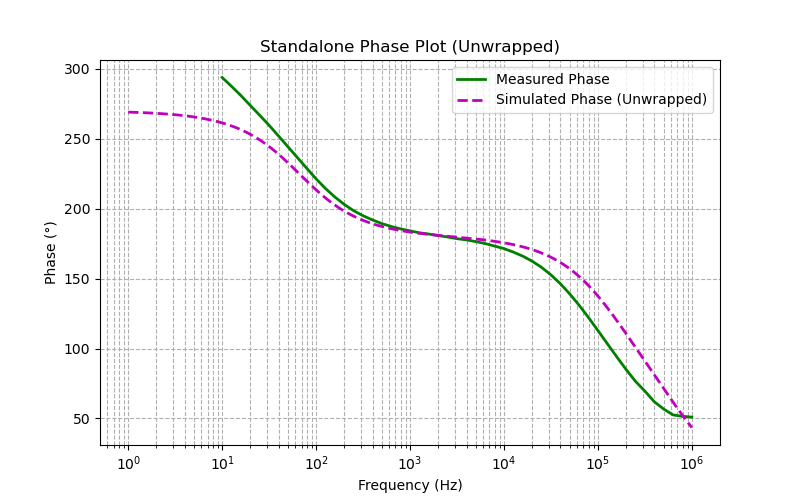
\includegraphics[width=1.0\linewidth]{Chapter_5/Lab_05_Phase_vs.png}
	\caption{Simulated vs Measured Phase}
	\label{Ch5_fig:5}
\end{figure}


\section{Python Code Listings}



\section{Conclusion}
This lab demonstrated the powerful role of negative feedback in modifying the behavior of a common source amplifier. By introducing a resistor from the drain to the gate of transistor $Q_1$​, the amplifier achieved improved DC stability without requiring a separate bias voltage. This feedback mechanism effectively stabilized the operating point and gain, making the circuit more predictable and less sensitive to parameter variations. Although the overall voltage gain was reduced, the trade-off resulted in a substantial increase in bandwidth, leading to a higher Gain-Bandwidth Product (GBW). The comparison between simulated and measured results showed good agreement, validating the effectiveness of the feedback design and confirming the accuracy of LTSpice simulations. The experiment reinforces the practical value of feedback in analog circuit design, particularly for improving linearity, stability, and frequency response.
\chapter{Lab 6 — MOS Differential Pair: Single-Ended vs Differential Signals}
% !TeX root = main.tex

%\setkeys{Gin}{draft}

%\singlespacing
%\onehalfspacing

\section{Lab Assignment Goals}
\vspace{.25cm}
\justifying
\par The objective of this lab was to investigate the behavior of a differential pair of MOS composed of $Q_1$ and $Q_2$, and to analyze the distinctions between single-ended and differential signaling, with particular emphasis on their effect on the common mode rejection ratio (CMRR). The circuit was implemented using the ALD1105 MOSFET array. Differential operation was examined to evaluate its effectiveness in enhancing noise rejection and improving signal integrity. LTSpice simulations were utilized to validate theoretical predictions. In addition, worst-case and Monte Carlo analyses were performed to assess variability and robustness.

\begin{center}
\begin{figure}[H]
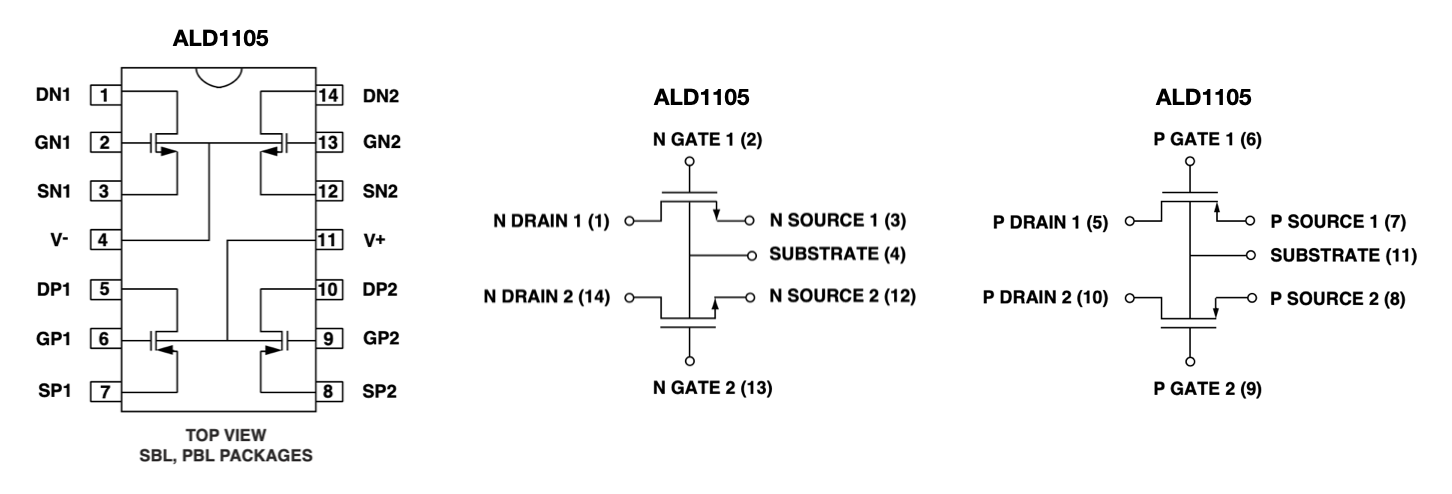
\includegraphics[scale=0.5]{Chapter_6/Lab_06_Image_1.png}
\caption{Pin-out and block diagram of the ALD1105. \textbf{Note: The body of the NMOS devices ($V^{-}$) was connected to the source, and the body of the PMOS devices ($V^{+}$) was connected to its source.}}
\label{Ch6_fig:1}
\end{figure}
\end{center}

\section{Experiment 1: MOS Differential Pair}

The MOS differential pair circuit, shown in Figure \ref{Ch6_fig:1}, was constructed with the Analog Discovery Studio. The following tasks were completed:

\begin{itemize}
    \item Resistances $R_{D}$ and $R_{CS}$ were measured and recorded in the summary table.
    \item The DC operating point was determined by measuring the node voltages and calculating the drain currents. The results were documented in the summary table.
\end{itemize}

\begin{itemize}
    \item{One of the most common questions asked is the difference between single-ended and differential signal inputs, and what applications they should be considered in.}
    \cite{dwyeromega2025}
\end{itemize}

\begin{center}
\begin{circuitikz}[american,scale=0.8]
\ctikzset{tripoles/mos style=arrows}
\draw
(-3,0) node[nmos,scale=2] (Q1) {}
(3,0) node[nmos,scale=2,xscale=-1] (Q2) {}
(Q1.center) node[right] {$Q_{1}$}
(Q2.center) node[left] {$Q_{2}$}
(Q1.S) -- (Q2.S)
(Q1.D) to[R=$R_{D}$] ++(0,3) node[vdd] {$+V_{DD}$}
(Q2.D) to[R=$R_{D}$] ++(0,3) node[vdd] {$+V_{DD}$}
(Q1.G) to[short,-o] ++(-0.5,0) node[left] {$v_{I1}$}
(Q2.G) to[short,-o] ++(0.5,0) node[right] {$v_{I2}$}
(Q1.S) to[open] ++(3,0) to[R=$R_{CS}$,*-] ++(0,-3) node[vss] {$-V_{SS}$}
(Q1.D) to[short,*-o] ++(-1,0) node[left] {$V_{X}$}
(Q1.D) to[short,-o] ++(1,0) node[right] {$-$}
(Q2.D) to[short,*-o] ++(1,0) node[right] {$V_{Y}$}
(Q2.D) to[short,-o] ++(-1,0) node[left] {$+$} to[open] ++(-1.55,0) node[left] {$v_{o}$}
;
\end{circuitikz}
\vspace{.5cm}
\par
Circuit Parameters: $V_{DD} = 12$ V, $-V_{SS} = -12$ V, $R_{D} = 18$k $\Omega$, $R_{CS} = 10$k $\Omega$, $V_{I1} = V_{I2} = 0$ V
\vspace{.5cm}
\emph{MOS Differential Pair Circuit}
\label{Ch6_fig:3}
\end{center}

\section{Experiment 2: AC Response}
\justifying{
The AC response of the differential pair was evaluated by determining the differential gain, the common-mode gain, and calculating the common-mode rejection ratio (CMRR). Measurements were performed for single-ended output (at node $V_{Y}$ with respect to the ground) and differential output (measuring voltage across nodes $V_{Y}$ and $V_{X}$). The following procedures were followed:}

\begin{itemize}
    \item For the differential input, a sinusoidal signal was applied to the positive input terminal and an equal but opposite phase signal was applied to the negative terminal, while both function generators were synchronized and biased appropriately.
    \item For common-mode input, identical sinusoidal signals were applied to both input terminals without phase offset. 
    \item Both wave generators were synchronized and appropriately biased.
    \item During AC analysis in LTSpice, the measured resistor values were used.
    \item The results were documented in the summary tables that have been provided on the following pages.
\end{itemize}

\begin{center}
	\begin{table}[H]
		\renewcommand{\arraystretch}{0.95}
		\begin{tabular}{ | >{\centering\arraybackslash} m{2.5cm} | >{\centering\arraybackslash} m{2.5cm} |  >{\centering\arraybackslash} m{2.5cm} |}
			\hline
			Quantity & Measured & Units \\ \hline
			$R_{D}$ & 18.025 & k$\Omega$ \\ \hline
			$R_{D}$ & 17.975 & k$\Omega$ \\ \hline
			$R_{CS}$ & 9.839 & k$\Omega$ \\ \hline
		\end{tabular}
	\caption{Resistor Summary}	
	\end{table}
\end {center}

\begin{table}[H]
\renewcommand{\arraystretch}{0.95}
\begin{tabular}{ | >{\centering\arraybackslash} m{2.5cm} | >{\centering\arraybackslash} m{2.5cm} |  >{\centering\arraybackslash} m{2.5cm} | >{\centering\arraybackslash} m{2.5cm} | >{\centering\arraybackslash} m{2.5cm} |}
\hline
\multicolumn{5}{|c|}{DC Operating Point}        \\ \hline
Device & Quantity & Simulated  & Measured & Units \\ \hline
\multirow{5}{*}{$Q_{1}$} & $I_{D}$  & 562.943 & 483.141 & $\mu$A   \\ \cline{2-5} 
                  & $|V_{OV}|$ & 1.407 & 1.141 & V \\ \cline{2-5} 
                  &  $V_{G}$ & 0.000 & 0.000 & V  \\ \cline{2-5} 
                  & $V_{D}$ & 3.063 & 2.896 & V \\ \cline{2-5} 
                  & $V_{S}$ & -1.891 & -1.820 & V \\ \hline
\multirow{5}{*}{$Q_{2}$} & $I_{D}$  & 558.043 & 524.011 & $\mu$A   \\ \cline{2-5} 
                  & $|V_{OV}|$ & 1.407 & 1.140 & V \\ \cline{2-5} 
                  &  $V_{G}$ & 0.000 & 0.000 & V  \\ \cline{2-5} 
                  & $V_{D}$ & 2.060 & 2.011 & V \\ \cline{2-5} 
                  & $V_{S}$ & -1.700 & -1.819 & V \\ \hline
\end{tabular}
\end{table}

\section{Background}
\justifying
In contrast to single-ended signaling, where the signal is measured with respect to a fixed potential (usually ground), differential signaling uses two complementary signals referenced to a common-mode voltage. 
\cite{razaviDifferentialPair}
This configuration provides several advantages:
\begin{itemize}
    \item \textbf{Immunity to environmental noise}: External interference affects both lines equally, and the differential measurement cancels out this noise.
    \item \textbf{Rejection of power supply noise}: Voltage fluctuations in the supply appear as common-mode noise, which is rejected by the differential pair.
    \item \textbf{Reduction of coupled noise}: Crosstalk and interference from adjacent signal lines are minimized.
\end{itemize}
\cite{palermoLab6}


\newpage

\begin{center}
	\renewcommand{\arraystretch}{1.2}
	\begin{table}[H]
	\begin{tabular}{ | >{\centering\arraybackslash} m{3.5cm} |  >{\centering\arraybackslash} m{3cm} | >{\centering\arraybackslash} m{3cm} | >{\centering\arraybackslash} m{2cm} |}
	\hline
	\multicolumn{4}{|c|}{AC Summary - Single Ended}        \\ \hline
	Quantity & Simulated  & Measured & Units \\ \hline
	$A_{d}$  & 6.018 & 6.205 & V/V   \\ \cline{1-4} 
	$A_{d}$ & 15.580 & 15.801 & dB \\ \cline{1-4} \hline
	 &  &  &  \\ \hline
	$A_{cm}$  & 0.840 & 0.499 & V/V   \\ \cline{1-4}
	$A_{cm}$ & -1.515 & -5.924 & dB \\ \cline{1-4} \hline
	 &  &  &  \\ \hline
	CMRR  & 17.104 & 21.724 & dB   \\ \cline{1-4}
\end{tabular}
\caption{AC Summary Table - Single Ended Output}
\end{table}

\end{center}

\begin{center}
\renewcommand{\arraystretch}{1.2}
\begin{table}[H]
\begin{tabular}{ | >{\centering\arraybackslash} m{3.5cm} |  >{\centering\arraybackslash} m{3cm} | >{\centering\arraybackslash} m{3cm} | >{\centering\arraybackslash} m{2cm} |}
\hline
\multicolumn{4}{|c|}{AC Summary - Differential}        \\ \hline
Quantity & Simulated  & Measured & Units \\ \hline
$A_{d}$  & 12.020 & 12.024 & V/V   \\ \cline{1-4} 
$A_{d}$ & 21.598 & 21.578 & dB \\ \cline{1-4} \hline
 &  &  &  \\ \hline
$A_{cm}$  & 0.001 & 0.053 & V/V   \\ \cline{1-4}
$A_{cm}$ & -61.379 & -26.760 & dB \\ \cline{1-4} \hline
 &  &  &  \\ \hline
CMRR  & 59.872 & 48.328 & dB   \\ \cline{1-4}
\end{tabular}
\caption{AC Summary Table - Differential Output}
\end{table}
\end{center}

%\newpage
\textbf{\textcolor{black}{Calculations and Methodology:}}
\vspace{0.3cm}

\noindent
\[
V_P = V_{in1} - V_{GS1} = V_{in2} - V_{GS2}
\]
\[
V_{in1} - V_{in2} = V_{GS1} - V_{GS2}
\]

% \textbf{\textcolor{black}{Equation (1):}}
\begin{tcolorbox}[colback=white,colframe=black,title=]
\begin{equation}
V_{in1} - V_{in2} = V_{GS1} - V_{GS2}
\end{equation}
\end{tcolorbox}

\vspace{0.5cm}

\noindent
\textbf{\textcolor{black}{Assuming $M_1$ and $M_2$ in saturation:}}
\[
(V_{GS} - V_{TH})^2 = \frac{2 I_D}{\mu_n C_{ox} \frac{W}{L}}
\]

% \textbf{\textcolor{black}{Equation (2):}}
\begin{tcolorbox}[colback=white,colframe=black,title=]
\begin{equation}
{V_GS} = \sqrt{\frac{2 I_D}{\mu_n C_{ox} \frac{W}{L}}} + {V_TH}
\end{equation}
\end{tcolorbox}

\begin{tikzpicture}[remember picture, overlay]
\node at (13.8,4.3) {\textcircled{2}};
\end{tikzpicture}

\vspace{0.5cm}

\noindent
\textbf{\textcolor{black}{From Eq. 1 \& 2:}}
\[
V_{in1} - V_{in2} = \sqrt{\frac{2 I_{D1}}{\mu_n C_{ox} \frac{W}{L}}} 
- \sqrt{\frac{2 I_{D2}}{\mu_n C_{ox} \frac{W}{L}}}
\]

\vspace{0.5cm}

\noindent
\textbf{\textcolor{black}{Squaring both sides, and since:}} \quad $I_{SS} = I_{D1} + I_{D2}$

\begin{tcolorbox}[colback=white,colframe=black,title=]
\begin{equation}
{(V_{in1} - V_{in2})^2 = \frac{2}{\mu_n C_{ox} \frac{W}{L}} \left (I_{SS} - 2 \sqrt{I_{D1} I_{D2}} \right)}
\end{equation}
\end{tcolorbox}

\vspace{0.5cm}

\noindent
% \textbf{\textcolor{blue}{Previous equation can be written:}}
\begin{equation}
\frac{\mu_n C_{ox}}{2} \frac{W}{L} (V_{in1} - V_{in2})^2 - I_{SS} = -2 \sqrt{I_{D1} I_{D2}}
\end{equation}

\vspace{0.25cm}

\noindent
% \textbf{\textcolor{blue}{Squaring the two sides, and since:}}
\begin{equation}
4 I_{D1} I_{D2} = (I_{D1} + I_{D2})^2 - (I_{D1} - I_{D2})^2 = I_{SS}^2 - (I_{D1} - I_{D2})^2
\end{equation}

\vspace{0.25cm}

\noindent
% \textbf{\textcolor{blue}{We arrive at:}}
\begin{equation}
(I_{D1} - I_{D2})^2 = -\frac{1}{4} \left( \frac{\mu_n C_{ox}}{W/L} \right)^2 (V_{in1} - V_{in2})^4 
+ I_{SS} \frac{\mu_n C_{ox}}{W/L} (V_{in1} - V_{in2})^2
\end{equation}

\vspace{0.25cm}

% \begin{tcolorbox}[colback=white,colframe=black,title=]
\begin{equation}
I_{D1} - I_{D2} = \frac{\mu_n C_{ox}}{2} \frac{W}{L}(V_{in1} - V_{in2}) 
\sqrt{\frac{4 I_{SS}}{\mu_n C_{ox} \frac{W}{L}} - (V_{in1} - V_{in2})^2}
\end{equation}
% \end{tcolorbox}

\vspace{0.25cm}

\noindent
% \textbf{\textcolor{blue}{Previous equation can be written:}}
\begin{equation}
\frac{\mu_n C_{ox}}{2} \frac{W}{L} (V_{in1} - V_{in2})^2 - I_{SS} = -2 \sqrt{I_{D1} I_{D2}}
\end{equation}

\vspace{0.25cm}

\noindent
% \textbf{\textcolor{blue}{Squaring the two sides, and since:}}
\begin{equation}
4 I_{D1} I_{D2} = (I_{D1} + I_{D2})^2 - (I_{D1} - I_{D2})^2 = I_{SS}^2 - (I_{D1} - I_{D2})^2
\end{equation}

\vspace{0.25cm}

\noindent
% \textbf{\textcolor{blue}{We arrive at:}}
\begin{equation}
(I_{D1} - I_{D2})^2 = -\frac{1}{4} \left( \frac{\mu_n C_{ox}}{W/L} \right)^2 (V_{in1} - V_{in2})^4 
+ I_{SS} \frac{\mu_n C_{ox}}{W/L} (V_{in1} - V_{in2})^2
\end{equation}

\vspace{0.25cm}

\begin{tcolorbox}[colback=white,colframe=black,title=]
\begin{equation}
I_{D1} - I_{D2} = \frac{\mu_n C_{ox}}{2} \frac{W}{L}(V_{in1} - V_{in2}) 
\sqrt{\frac{4 I_{SS}}{\mu_n C_{ox} \frac{W}{L}} - (V_{in1} - V_{in2})^2}
\end{equation}
\end{tcolorbox}

\vspace{0.25cm}

\noindent
\begin{center}
Let \quad $\Delta V_{in} = V_{in1} - V_{in2}$ \quad and \quad $\Delta I_D = I_{D1} - I_{D2}$
\end{center}

\vspace{0.25cm}

\noindent

\textbf{\textcolor{black}{Deriving Eq. (3) with respect to $\Delta V_{in}$:}}
\begin{tcolorbox}[colback=white,colframe=black,title=]
\begin{equation}
G_m = \frac{\partial \Delta I_D}{\partial \Delta V_{in}} 
= \frac{\mu_n C_{ox}}{2} \frac{W}{L} 
\sqrt{\frac{4 I_{SS}}{\mu_n C_{ox} \frac{W}{L}} - 2 \Delta V_{in}^2}
\end{equation}
\end{tcolorbox}

\vspace{0.75cm}

\noindent
For \quad $\Delta V_{in} = 0 :$ \quad 
\[
G_m = \sqrt{\mu_n C_{ox} \frac{W}{L} I_{SS}}
\]

\vspace{0.55cm}

\noindent
\textbf{\textcolor{black}{Since:}}
\[
V_{out1} - V_{out2} = V_{DD} - I_{D1} R_{D1} - V_{DD} + I_{D2} R_{D2}
\]
\[
\Delta V_{out} = \Delta I_D R_D
\]
\[
\Delta V_{out} = G_m \Delta V_{in} R_D
\]

\vspace{0.5cm}

\newpage

\noindent
\textbf{\textcolor{black}{Small signal differential voltage gain:}}
\begin{tcolorbox}[colback=white,colframe=black,title=]
\begin{equation}
|A_v| = \frac{\Delta V_{out}}{\Delta V_{in}} = G_m R_D = \sqrt{\mu_n C_{ox} \frac{W}{L} \cdot I_SS \cdot R_D}
\end{equation}
\end{tcolorbox}

\vspace{0.5cm}
\noindent
$\Delta V_{in1}$ is when $I_{D1} = I_{SS}$

\[
\Delta V_{in1} = V_{GS1} - V_{TH1}
\quad \Rightarrow \quad 
\Delta V_{in1} = \sqrt{\frac{2 I_{SS}}{\mu_n C_{ox} \frac{W}{L}}}
\]

\vspace{0.3cm}
\textbf{\textcolor{black}{Voltage and Current Relationship:}}
\begin{tcolorbox}[colback=white,colframe=black,title=]
\begin{equation}
I_{D1} - I_{D2} = \frac{\mu_n C_{ox}}{2} \frac{W}{L}(V_{in1} - V_{in2})
\sqrt{\frac{4 I_{SS}}{\mu_n C_{ox} \frac{W}{L}} - (V_{in1} - V_{in2})^2}
\end{equation}
\end{tcolorbox}

\vspace{0.75cm}

\textbf{\textcolor{black}{Equation for Transconductance:}}
\begin{tcolorbox}[colback=white,colframe=black,title=]
\begin{equation}
G_m = \frac{\mu_n C_{ox}}{2} \frac{W}{L}
\sqrt{\frac{4 I_{SS}}{\mu_n C_{ox} \frac{W}{L}} - 2 \Delta V_{in}^2}
\end{equation}
\end{tcolorbox}

\vspace{1cm}

\begin{figure}[H]
\centering
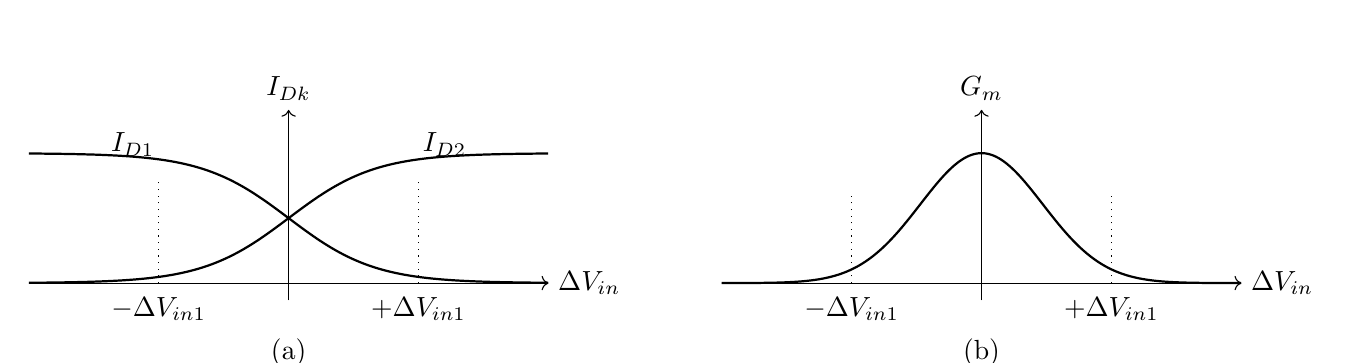
\begin{tikzpicture}[scale=1.1]

% ==== Left Plot - ID1 and ID2 ====
\begin{scope}[xshift=-4cm]

\draw[->] (-3,0) -- (3,0) node[right] {$\Delta V_{in}$};
\draw[->] (0,-0.2) -- (0,2) node[above] {$I_{Dk}$};

% Currents - ID1 and ID2
\draw[thick, domain=-3:3, samples=200, smooth]
plot (\x, {1.5/(1+exp(2*\x))});
\draw[thick, domain=-3:3, samples=200, smooth]
plot (\x, {1.5/(1+exp(-2*\x))});

% Labels
\node at (-1.8,1.6) {$I_{D1}$};
\node at (1.8,1.6) {$I_{D2}$};

% Vertical dashed lines
\draw[dotted] (-1.5,0) -- (-1.5,1.2);
\draw[dotted] (1.5,0) -- (1.5,1.2);
\node at (-1.5,-0.3) {$-\Delta V_{in1}$};
\node at (1.5,-0.3) {$+\Delta V_{in1}$};

% (a) label
\node at (0,-0.8) {(a)};
\end{scope}

% ==== Right Plot - Gm ====
\begin{scope}[xshift=4cm]
% Axes
\draw[->] (-3,0) -- (3,0) node[right] {$\Delta V_{in}$};
\draw[->] (0,-0.2) -- (0,2) node[above] {$G_m$};

% Gm plot
\draw[thick, domain=-3:3, samples=200, smooth]
plot (\x, {1.5*exp(-(\x)^2)});

% Vertical dashed lines
\draw[dotted] (-1.5,0) -- (-1.5,1.0);
\draw[dotted] (1.5,0) -- (1.5,1.0);
\node at (-1.5,-0.3) {$-\Delta V_{in1}$};
\node at (1.5,-0.3) {$+\Delta V_{in1}$};

% (b) label
\node at (0,-0.8) {(b)};
\end{scope}

\end{tikzpicture}
\caption{(a) Plot of Current vs. Differential Input Voltage, (b) Plot of Transconductance}
\end{figure}

\clearpage

\cite{aboushady2016}

\cite{dynapar2025}

\cite{razaviDifferentialPair}


\newpage

\section{Single-ended vs Differential Input Comparison Plot}
\vspace*{2cm}
\begin{figure}[H]
    \centering
    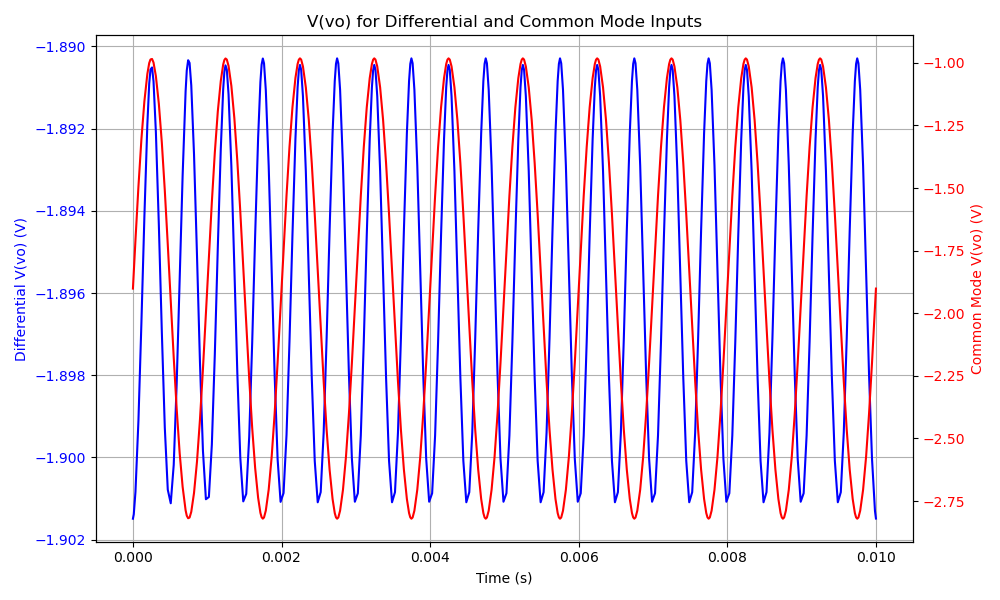
\includegraphics[width=0.95\linewidth]{Chapter_6/Lab-06-LTSpice-Plot.png}
    \caption{In-Phase vs Out-of-Phase Plots of Simulated V(vo)}
    \label{Ch6_fig:4}
\end{figure}

\section{Python Code Listings}

The Python code for differential pair analysis can be found in the Appendix (\cref{lst:Ch6:List1}).

\section{Conclusion}
The lab successfully demonstrated the behavior and advantages of a MOS differential pair, specifically highlighting its performance using the ALD1105 MOSFET array. Through both theoretical analysis and practical implementation, the lab emphasized the superiority of differential signaling over single-ended signaling in terms of noise rejection and signal integrity. The measured DC operating points closely matched simulation predictions, validating the circuit’s proper biasing and symmetrical configuration.

AC analysis further confirmed the benefits of differential operation. The differential gain was significantly higher and more stable, while the common-mode gain was drastically reduced compared to the single-ended configuration. This led to a much higher common-mode rejection ratio (CMRR), both in simulation and measurement, for the differential output. The measured CMRR increased from $21.7$ dB (single-ended) to $48.3$ dB (differential), demonstrating the effectiveness of the differential pair in suppressing common-mode noise.

Theoretical derivations, supported by LTSpice simulations, aligned with experimental results, strengthening the understanding of current steering mechanisms and transconductance behavior in MOS differential amplifiers. In summary, the lab clearly illustrated the functional and practical benefits of differential signaling in analog circuit design, particularly in enhancing noise immunity and ensuring signal fidelity in mixed-signal environments.

\clearpage
\printbibliography[heading=subbibliography]
\chapter{Lab 7 — MOS Differential Pair: Current Mirror}
% !TeX root = main.tex

%\setkeys{Gin}{draft}
%\onehalfspacing
	
\section{Lab Assignment Goals}

\justifying 
\par
This lab investigated the MOS differential pair composed of transistors $Q_1$ and $Q_2$ with a current mirror load formed by $Q_3$ and $Q_4$, functioning as a differential to single-ended amplifier stage. The common-mode rejection ratio (CMRR) was analyzed. The circuit was implemented using the ALD1105 MOSFET array. Differential operation was examined to evaluate its effectiveness in noise rejection and signal integrity. LTSpice simulations were performed to validate theoretical predictions and support measurement techniques.

\begin{center}
\begin{figure}[h]
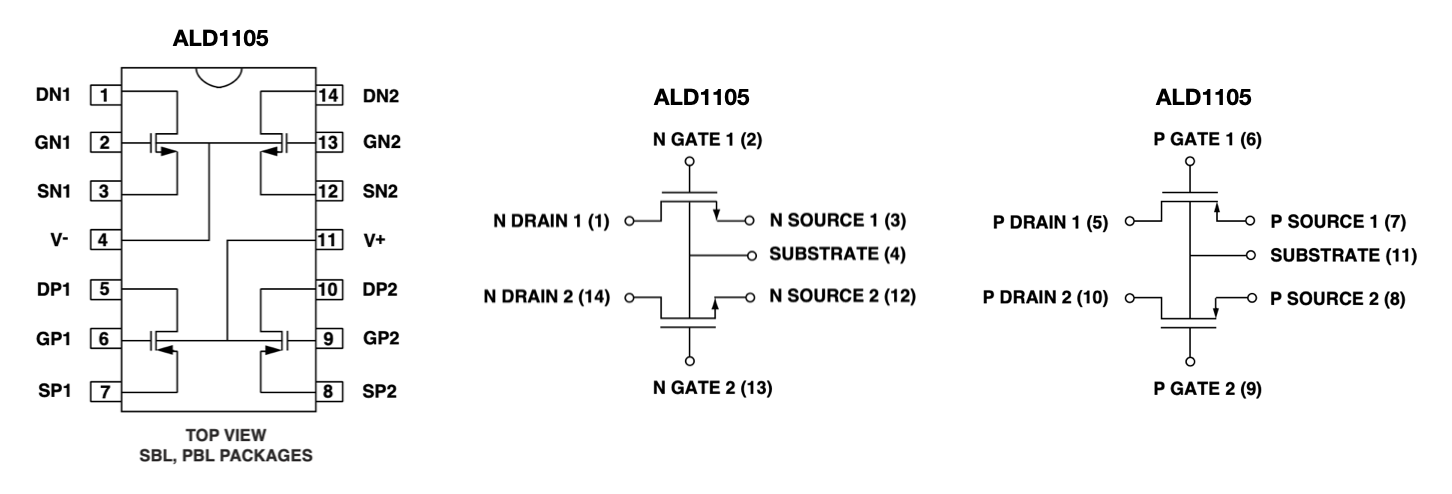
\includegraphics[scale=0.5]{Chapter_7/Lab_07_Image_1.png}
\caption{The pin-out and block diagram of the ALD1105. \textbf{Note: $V^{-}$ is the body of the NMOS devices and is connected to the source, and $V^{+}$ is the body of the PMOS devices, which is also connected to its source.}}
\label{Ch7_fig:1}
\end{figure}
\end{center}

\section{Experiment 1: MOS Differential Pair DC Measurements}

The MOS differential pair circuit was constructed on the Analog Discovery Studio as shown below:

\begin{itemize}
    \item The resistance $R_{CS}$ was measured and recorded.
    \item The DC operating point was determined by measuring node voltages and calculating the corresponding currents.
\end{itemize}

\begin{center}
\begin{circuitikz}[american,scale=0.8]
\ctikzset{tripoles/mos style=arrows}
\node at (0,9.5) {\Large \textbf{Common-Mode Input}};
\draw

(-3,0) node[nmos,scale=2] (Q1) {}
(3,0) node[nmos,scale=2,xscale=-1] (Q2) {}
(-3,5) node[pmos,scale=2, xscale=-1] (Q3) {}
(3,5) node[pmos,scale=2] (Q4) {}
(Q1.center) node[right] {$Q_{1}$}
(Q2.center) node[left] {$Q_{2}$}
(Q3.G) -- (Q4.G)
(Q1.S) -- (Q2.S)
(Q1.D) -- (Q3.D)
(Q2.D) -- (Q4.D)
(Q3.S) node[vdd] {$V_{DD}$}
(Q4.S) node[vdd] {$V_{DD}$}
(Q1.G) to[short,-o] ++(-0.5,0) node[left] {$v_{I1}$}
(Q2.G) to[short,-o] ++(0.5,0) node[right] {$v_{I2}$}
(Q1.S) to[open] ++(3,0) to[R=$R_{CS}$,*-] ++(0,-3) node[vss] {$-V_{SS}$}
(Q2.D) to[open] ++(0,0.5) to[short,*-o] ++(1,0) node[right] {$v_{O}$}
(Q1.D) to[open] ++(0,0.5) to[short,*-] ++(3,0) to[short,-*] ++(0,2.557)
;	
\end{circuitikz}

\vspace{.5cm}

$V_{DD} = 12$ V \hspace{0.5cm}  $-V_{SS} = -12$ V  \hspace{0.5cm}  $R_{CS} = 10$k $\Omega$ \hspace{0.5cm} $V_{I1}=V_{I2} = 0$ V

\vspace{.5cm}
\end{center}

\subsection*{Observations}

The simulated values for the drain currents ($I_D$) based on node voltages ($V_G$ and $V_S$) are all the same while measured values differ for the pairs formed by Q1 with Q2 and Q3 with Q4. Specifically:

\begin{itemize}
    \item \textbf{Q1/Q2 (NMOS)}: $I_D = 514.000$ $\mu\text{A}$ (simulated)
    \item \textbf{Q3/Q4 (PMOS)}: $I_D = 514.000$ $\mu\text{A}$ (simulated)
\end{itemize}

Compared to the measured values:
\begin{itemize}
    \item \textbf{Q1}: 663.487 $\mu$A,\quad \textbf{Q2}: 343.301 $\mu$A (measured)
    \item \textbf{Q3}: 663.487 $\mu$A,\quad \textbf{Q4}: 343.301 $\mu$A (measured)
\end{itemize}

\newpage

\noindent\textbf{Observations:}
\begin{itemize}
    \item The measured current for Q2 is lower than the simulated value. This discrepancy is likely due to the quadratic relationship between drain current and overdrive voltage ($V_{ov}$), which makes $I_D$ highly sensitive to small changes in $V_{ov}$, $\lambda$ is another likely candidate for as a cause behind this discrepancy \cite{rajesh_differential_2014}.
    \item Although Q2 shares the same $V_S$ and $V_{G}$ as Q1, and also taking into consideration that $I_{D3}$ and $I_{D4}$ should mirror one another, this does not result in an identical measured current. However, the measured current for Q2 is significantly lower, suggesting device mismatch or the influence of channel-length modulation (Early effect) \cite{fonstad_mit2009}.
\end{itemize}

\justifying

A MOS differential pair with a current mirror load is used to amplify differential signals while rejecting common-mode noise. This topology is foundational in analog integrated circuit design.

\begin{itemize}
    \item \textbf{Structure}: Transistors $Q_1$ and $Q_2$ form the differential pair, and $Q_3$, $Q_4$ implement the current mirror load \cite{fonstad_mit2009}.
    \[
    I_{D1} = I_{D2} = \frac{I_{R_{CS}}}{2}
    \]
    when \( V_{I1} = V_{I2} \).
    \item \textbf{Active Load Benefits}:
    \begin{itemize}
        \item Converts differential current to single-ended output \cite{rajesh_differential_2014}.
        \item Increases gain vs resistive loads:
        \[
        A_{v,d} \approx g_m \cdot R_{out} \quad \text{with } R_{out} \gg R_{resistive}
        \]
        \item Improves common-mode rejection ratio (CMRR):
        \[
        \text{CMRR} = \left| \frac{A_{d}}{A_{cm}} \right|
        \]
    \end{itemize}
    \item \textbf{Matching}:
    \begin{itemize}
        \item Requires \( Q_1 = Q_2 \) and \( Q_3 = Q_4 \) for optimal performance.
        \item Imbalances introduce input offset voltage:
        \[
        V_{OS} = \frac{I \cdot \Delta R}{2}
        \]
    \end{itemize}
    \item \textbf{Common-mode suppression}:
    \[
    V_{D1} = V_{D2} \quad \Rightarrow \quad V_O = 0 \quad \text{(ideal)}
    \]
    Common-mode gain will approach zero as the impedance of $R_{CS}$ increases \cite{deo2020bimos}.
\end{itemize}


\newpage

\section{Experiment 2: MOS Differential Pair AC Response}

The differential and common-mode gains were determined using measurement techniques, and the common-mode rejection ratio (CMRR) was calculated. The output was taken from node $v_{O}$ with respect to ground.

\begin{itemize}
    \item The differential input was applied using two synchronized sinusoidal signals, equal in magnitude but opposite in phase.
    \item The common-mode input was created by applying the same synchronized signal to both terminals with appropriate biasing.
    \item Measured resistor values were used for AC analysis in LTSpice.
    \item Measured data was recorded in the following summary tables.
\end{itemize}

% \newpage

\begin{center}
\begin{circuitikz}[american,scale=0.8]
\ctikzset{tripoles/mos style=arrows}
\node at (0,9.5) {\Large \textbf{Difference-Mode Inputs}};

\draw

(-3,0) node[nmos,scale=2] (Q1) {}
(3,0) node[nmos,scale=2,xscale=-1] (Q2) {}
(-3,5) node[pmos,scale=2, xscale=-1] (Q3) {}
(3,5) node[pmos,scale=2] (Q4) {}
(Q1.center) node[right] {$Q_{1}$}
(Q2.center) node[left] {$Q_{2}$}
(Q3.center) node[right] {$Q_{3}$}
(Q4.center) node[left] {$Q_{4}$}
(Q3.G) -- (Q4.G)
(Q1.S) -- (Q2.S)
(Q1.D) -- (Q3.D)
(Q2.D) -- (Q4.D)
(Q3.S) node[vdd] {$V_{DD}$}
(Q4.S) node[vdd] {$V_{DD}$}
(Q1.G) to[short,-o] ++(-0.5,0) node[left] {$\frac{+v_{I}}{2}$}
(Q2.G) to[short,-o] ++(0.5,0) node[right] {$\frac{-v_{I}}{2}$}
(Q1.S) to[open] ++(3,0) to[R=$R_{CS}$,*-] ++(0,-3) node[vss] {$-V_{SS}$}
(Q2.D) to[open] ++(0,0.5) to[short,*-o] ++(1,0) node[right] {$v_{O}$}
(Q1.D) to[open] ++(0,0.5) to[short,*-] ++(3,0) to[short,-*] ++(0,2.557)
;	
\end{circuitikz}

\vspace{.5cm}

$V_{DD} = 12$ V \hspace{0.5cm}  $-V_{SS} = -12$ V  \hspace{0.5cm}  $R_{CS} = 10$k $\Omega$ \hspace{0.5cm} $V_{I1}=V_{I2} = 0$ V

\vspace{.5cm}
\end{center}

\begin{itemize} 
    \item The circuit utilizes a current mirror load, which allows differential-mode current doubling and suppresses common-mode currents, making it effective for single-ended output without sacrificing gain \cite{fonstad_mit2009}.
    \item The differential-mode gain for a current mirror loaded differential pair is approximated as:
    \[
    A_{v,d} \approx \frac{2g_{m3}}{g_{o2} + g_{o4} + G_L}
    \]
\end{itemize}
\newpage
\par
where \(g_{m3}\) is the transconductance of the current mirror transistor, \(g_{o2}, g_{o4}\) are the output conductance, and \(G_L\) is the load conductance \cite{fonstad_mit2009}.
\par
\begin{itemize}
    \item In contrast, the common-mode gain is significantly smaller:
    \begin{center}
    \item $A_{v,cm} \approx \frac{g_{ob}}{2(g_{m2} + g_{o4} + G_L)}$    
    \end{center}
\end{itemize}
This results in excellent rejection of common-mode noise, contributing to a high CMRR \cite{fonstad_mit2009}.
\begin{itemize}
        
    \item From the small-signal model:
    \[
    \text{CMRR} = \frac{A_{v,d}}{A_{v,cm}} \approx \frac{2g_{m3}}{g_{ob}} \cdot \frac{g_{m2}}{g_{o2} + g_{o4} + G_L}
    \]
\end{itemize}
High values of \(g_m\) and low output conductance are favorable for achieving high CMRR \cite{fonstad_mit2009}.
\begin{itemize}
    
    \item The implementation also benefits from the mirrored topology which ensures that any common-mode signal appears equally at both inputs and is \textbf{effectively canceled out}, a principle demonstrated in both theoretical and experimental studies \cite{razaviDifferentialPair}.
    
    \item According to \cite{palermoLab6}, a finite output impedance in the tail current source slightly reduces CMRR due to common-mode to differential-mode conversion:
    \[
    A_{cm} \approx \frac{1}{1 + 2g_mR_{SS}}
    \]
    \item (for this experiment, $R_{SS} = R_{CS}$)
\end{itemize}
where \(R_{SS}\) is the source degeneration resistance. Ideally, this should be large.
\begin{itemize}
    \item The presence of mismatches (e.g., \(g_{m1} \neq g_{m2}\)) introduces additional differential components into the output in response to a purely common-mode input, reducing CMRR. This is quantified using:
    \[
    A_{CM \to DM} \approx \frac{(g_{m1} - g_{m2}) R_{SS}}{g_{m1} + g_{m2} + \dots}
    \]
    which highlights the importance of symmetric layout and transistor matching 
\cite{iiitd_lecture16}.
\end{itemize}

\begin{itemize}
    \item Overall, using a current mirror as an active load provides significant advantages in terms of:
        \begin{itemize}
            \item Converting differential signal to single-ended output efficiently
            \item Doubling the effective gain compared to resistive loads
            \item Minimizing common-mode gain
            \item Enabling high CMRR with compact layout
        \end{itemize}
    as emphasized in multiple foundational sources \cite{rajesh_differential_2014, fonstad_mit2009, iiitd_lecture16}.
\end{itemize}


\newpage

\begin{center}

\begin{table}[H]
\begin{tabular}{ | >{\centering\arraybackslash} m{2.5cm} | >{\centering\arraybackslash} m{2.5cm} |  >{\centering\arraybackslash} m{2.5cm} | >{\centering\arraybackslash} m{2.5cm} | >{\centering\arraybackslash} m{2.5cm} |}
\hline
\multicolumn{5}{|c|}{DC Operating Point}        \\ \hline
Device & Quantity & Simulated  & Measured & Units \\ \hline
\multirow{5}{*}{$Q_{1}$} & $I_{D}$ & 514.000 & 540.335 & $\mu$A   \\ \cline{2-5} 
& $|V_{OV}|$ & 1.267 & 1.365 & V \\ \cline{2-5} 
& $V_{G}$ & 0.000 & 0.000 & V  \\ \cline{2-5} 
& $V_{D}$ & 9.010 & 8.606 & V \\ \cline{2-5} 
& $V_{S}$ & -1.844 & -1.985 & V \\ \hline

\multirow{5}{*}{$Q_{2}$} & $I_{D}$  & 514.000 & 540.335 & $\mu$A   \\ \cline{2-5} 
& $|V_{OV}|$ & 1.267 & 1.365 & V \\ \cline{2-5} 
& $V_{G}$ & 0.000 & 0.000 & V  \\ \cline{2-5} 
& $V_{D}$ & 9.011 & 8.606 & V \\ \cline{2-5} 
& $V_{S}$ & -1.844 & -1.985 & V \\ \hline

\multirow{5}{*}{$Q_{3}$} & $I_{D}$  & 514.000 & 540.335 & $\mu$A   \\ \cline{2-5} 
& $|V_{OV}|$ & 2.343 & 2.394 & V \\ \cline{2-5} 
& $V_{G}$ & 9.010 & 8.606 & V  \\ \cline{2-5} 
& $V_{D}$ & 9.010 & 8.606 & V \\ \cline{2-5} 
& $V_{S}$ & 12.000 & 12.000 & V \\ \hline

\multirow{5}{*}{$Q_{4}$} & $I_{D}$  & 514.000 & 540.335 & $\mu$A   \\ \cline{2-5} 
& $|V_{OV}|$ & 2.343 & 2.394 & V \\ \cline{2-5} 
& $V_{G}$ & 9.010 & 8.606 & V  \\ \cline{2-5} 
& $V_{D}$ & 9.010 & 8.606 & V \\ \cline{2-5} 
& $V_{S}$ & 12.000 & 12.000 & V \\ \hline
\end{tabular}
\caption{DC Summary Table}
\end{table}

\newpage

\begin{table}[H]
\begin{tabular}{ | >{\centering\arraybackslash} m{2.5cm} | >{\centering\arraybackslash} m{2.5cm} |  >{\centering\arraybackslash} m{2.5cm} |}
\hline
Quantity & Measured & Units \\ \hline
$R_{CS}$ & 9.872 & k$\Omega$ \\ \hline
\end{tabular}
\caption{Resistor Summary}	
\end{table}

\begin{table}[H]
\begin{tabular}{ | >{\centering\arraybackslash} m{3.5cm} |  >{\centering\arraybackslash} m{3cm} | >{\centering\arraybackslash} m{3cm} | >{\centering\arraybackslash} m{2cm} |}
\hline
\multicolumn{4}{|c|}{AC Summary - Single Ended}        \\ \hline
Quantity & Simulated  & Measured & Units \\ \hline
$A_{d}$  & 44.888 & 24.161 & V/V   \\ \cline{1-4} 
$A_{d}$ & 33.040 & 27.662 & dB \\ \hline
$A_{cm}$  & 0.105 & 0.183 & V/V   \\ \cline{1-4}
$A_{cm}$ & -19.591 & -14.751 & dB \\ \hline
CMRR  & 52.632 & 42.413 & dB   \\ \cline{1-4}
\end{tabular}
\caption{AC Summary Table - Single Ended Output}
\end{table}
\end{center}
\newpage

\begin{figure}
    \centering
    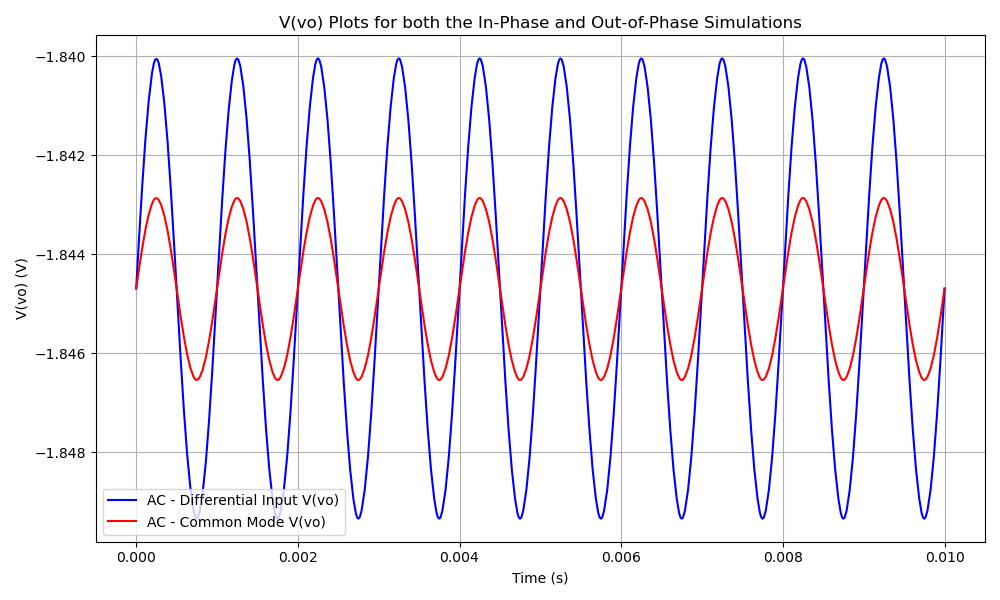
\includegraphics[width=0.95\linewidth]{Chapter_7/Lab_07_CM_vs_Diff_Plot.png}
    \caption{Differential Mode V(vo)}
    \label{Ch7_fig:2}
\end{figure}
\clearpage

\begin{figure}
    \centering
    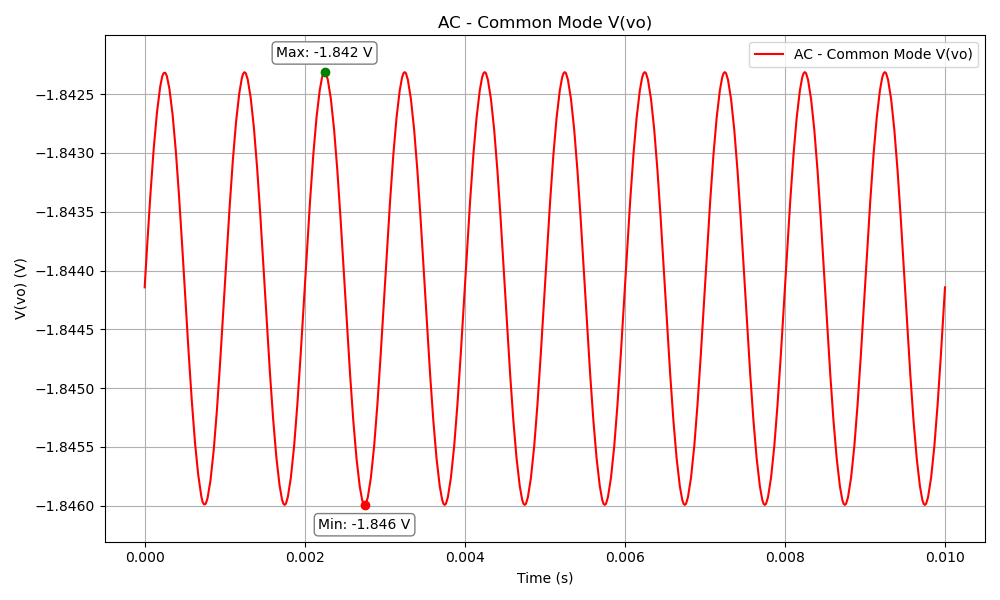
\includegraphics[width=0.95\linewidth]{Chapter_7/Lab_07_AC_CommonMode_vo_Plot.png}
    \caption{Common Mode V(vo)}
    \label{Ch7_fig:3}
\end{figure}
\clearpage

%\newpage
%\section*{Python Code used in Calculations}
%\lstinputlisting[language=Python]{Appendix/Python_Code/Lab_07_Table_1_DC_Summary_Placzek.py}
%\clearpage
\section{Python	Output: Simulated vs Measured \% Difference}
\vspace{0.25cm}
\begin{verbatim}
	|--------------------------------------------------------|
	|============== DC Percent Difference Table =============|
	| Dev | Quant |  Sim   | Meas  | Unit | Diff  | %Diff    |
	|-----|-------|--------|-------|------|-------|----------|
	| Q1  | ID    | 514.0  | 540.3 | uA   | 26.3  | 5.116    |
	| Q1  | VOV   | 1.267  | 1.365 | V    | 0.098 | 7.733    |
	| Q1  | VG    | 1.840  | 0.000 | V    | 1.840 | N/A  |
	| Q1  | VD    |10.900  | 8.606 | V    | 2.294 | 21.038   |
	| Q1  | VS    | 0.000  |-1.985 | V    | 1.985 | N/A      |
	| Q2  | ID    | 514.0  | 540.3 | uA   | 26.3  | 5.116    |
	| Q2  | VOV   | 1.267  | 1.365 | V    | 0.098 | 7.733    |
	| Q2  | VG    | 1.840  | 0.000 | V    | 1.840 | 100.000  |
	| Q2  | VD    |10.900  | 8.606 | V    | 2.294 | 21.038   |
	| Q2  | VS    | 0.000  |-1.985 | V    | 1.985 | N/A      |
	| Q3  | ID    | 514.0  | 540.3 | uA   | 26.3  | 5.116    |
	| Q3  | VOV   | 2.343  | 2.394 | V    | 0.051 | 2.177    |
	| Q3  | VG    |-2.990  | 8.606 | V    |11.596 | 388.125  |
	| Q3  | VD    |-2.990  | 8.606 | V    |11.596 | 388.125  |
	| Q3  | VS    | 0.000  |12.000 | V    |12.000 | N/A      |
	| Q4  | ID    | 514.0  | 540.3 | uA   | 26.3  | 5.116    |
	| Q4  | VOV   | 2.343  | 2.394 | V    | 0.051 | 2.177    |
	| Q4  | VG    |-2.990  | 8.606 | V    |11.596 | 388.125  |
	| Q4  | VD    |-2.990  | 8.606 | V    |11.596 | 388.125  |
	| Q4  | VS    | 0.000  |12.000 | V    |12.000 | N/A      |
	|--------------------------------------------------------|
	|========================================================|
\end{verbatim}

\section{Python Code Listings}

The Python implementations for the current mirror analysis can be found in the Appendix: DC Summary Calculations (\cref{lst:Ch7:List1}), AC Summary Calculations (\cref{lst:Ch7:List2}), and Data Analysis and Plots (\cref{lst:Ch7:List3}).

\section{Conclusion}
\vspace{0.25cm}
\justifying
This lab demonstrated the operation and advantages of a MOSFET differential pair using the ALD1105 IC. By constructing and analyzing the circuit both experimentally and through LTSpice simulations, we verified that differential signaling offers significant benefits over single-ended approaches. Notably, the differential configuration achieved a much higher common-mode rejection ratio (CMRR), with simulated and measured values of approximately $59.9$ dB and $48.3$ dB respectively, compared to $17.1$ dB and $21.7$ dB for single-ended output. These results confirm the superior noise rejection capabilities inherent to differential systems. Theoretical modeling was reinforced by close agreement between simulated and measured values for parameters such as differential gain and DC operating points. Overall, this lab emphasized the importance of differential signaling in high-fidelity analog design and the utility of simulation tools in predicting and optimizing circuit performance.

\clearpage
\printbibliography[heading=subbibliography]
\chapter{Lab 8 — VNA Measurement: De-Embedding S-Parameters}
% !TeX root = main.tex

%\setkeys{Gin}{draft}
\singlespacing
	
\section{Lab Assignment Goals}
\justifying
This laboratory experiment focused on the fundamentals of using a Vector Network Analyzer (VNA) to characterize the frequency-domain behavior of high-frequency components and networks. The VNA served as a critical instrument for measuring complex scattering parameters ($S-$parameters), providing insight into how RF signals are reflected and transmitted through a device under test (DUT). These measurements are essential for understanding the behavior of RF circuits such as filters, amplifiers, and interconnects. \cite{ieee370_2011}

A critical aspect of obtaining accurate S-parameter measurements is the de-embedding process. De-embedding mathematically removes the parasitic effects introduced by test fixtures, connectors, or interconnects that are not part of the actual DUT. Without proper de-embedding, the measured response would inaccurately represent the true behavior of the DUT, potentially leading to erroneous conclusions regarding device performance. \cite{nan2007dummyfills}

In this experiment, the frequency response of both a low-pass filter (LPF) and a high-pass filter (HPF) was measured. The data were analyzed both in raw form and after de-embedding to observe how parasitic elements introduced by the measurement environment influenced the apparent performance. Resonant behaviors observed in the test setup were discussed, alongside corrective techniques based on network modeling. \cite{amakawa2015comparative}

\section{S-Parameter De-embedding Methods}
\justifying

S-parameter de-embedding was conducted according to industry standards, specifically adhering to principles outlined by the IEEE Standard for Test Procedures for High-Frequency Transmission Lines on Printed Boards \cite{ieee370_2020}. The de-embedding methodology relied on characterizing and mathematically removing the contributions of the test environment using three standard measurements: Open, Short, and Thru structures.

% -----------------------------------------------------------------------------
% Measurement Fixture and De-Embedding Theory
% -----------------------------------------------------------------------------
\section{Measurement Fixture and De-Embedding Theory}
\justifying
All fixtures will add their own frequency-dependent errors to a device under test.
Generally, a DUT is measured while sandwiched between two coaxial test fixtures, and these fixtures are absolutely are necessary in order to perform measurements, so this is unavoidable. 
\cite{ieee370_2020} 
By modeling each fixture with an $S-$matrix ($S_{FI}$ on the input side and $S_{FO}$ on the output side) we can mathematically remove their influence via network transformations (Fig.~\ref{Ch8_fig:1}).

\begin{figure}[H]
\centering
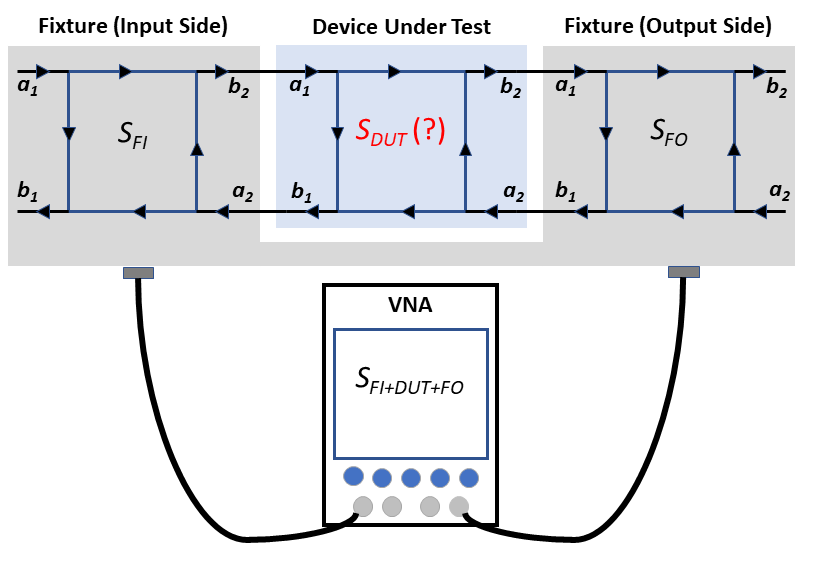
\includegraphics[width=0.9\textwidth]{Chapter_8/images/Lab_08_Figure1.png}
\caption{Block-diagram representation of the measurement topology: the VNA observes the cascade of input fixture, DUT, and output fixture. \cite{deembedding_part1} }
\label{Ch8_fig:1}
\end{figure}

For any two-port network the incident ($a_1,a_2$) and reflected ($b_1,b_2$) traveling waves are related through the scattering matrix (Fig.~\ref{Ch8_fig:2}):

\begin{equation}
\begin{pmatrix} b_1 \ b_2 \end{pmatrix} =
\begin{pmatrix} S_{11} & S_{12} \ S_{21} & S_{22} \end{pmatrix}
\begin{pmatrix} a_1 \ a_2 \end{pmatrix}.
\end{equation}

\begin{figure}[H]
\centering
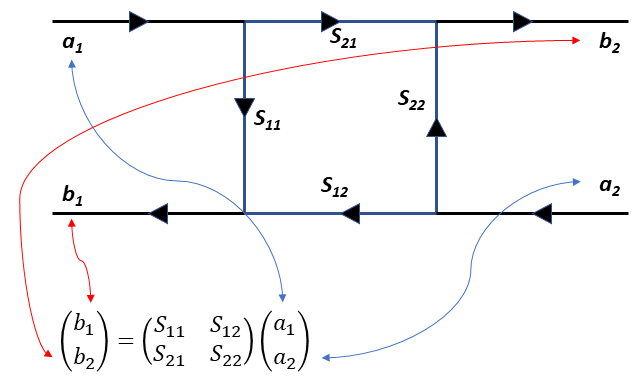
\includegraphics[width=0.75\textwidth]{Chapter_8/images/Lab_08_Figure2.png}
\caption{Directionality of the four scattering parameters for a reciprocal two-port. \cite{deembedding_part1} }
\label{Ch8_fig:2}
\end{figure}

Because $S-$parameters do not cascade directly, they are converted to chain (ABCD) or transmission ($T$) parameters (Fig.~\ref{Ch8_fig:3}):

\begin{align}
T_{11} &= -\frac{S_{11}S_{22}-S_{12}S_{21}}{S_{21}}, & T_{12} &= \frac{S_{11}}{S_{21}},\
T_{21} &= -\frac{S_{22}}{S_{21}}, & T_{22} &= \frac{1}{S_{21}}.
\end{align}

\begin{figure}[H]
\centering
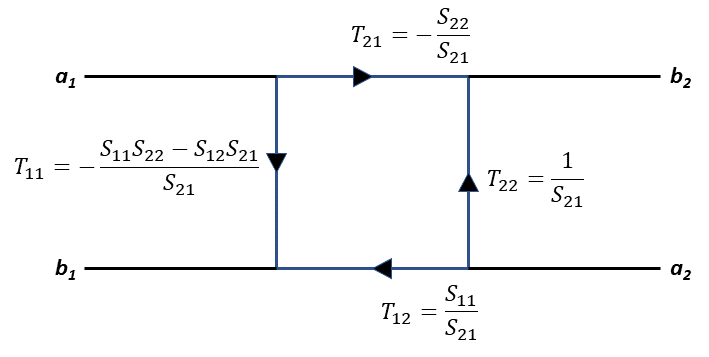
\includegraphics[width=0.75\textwidth]{Chapter_8/images/Lab_08_Figure3.png}
\caption{Formulae for converting $S-$parameters to $T$-parameters. \cite{deembedding_part1} }
\label{Ch8_fig:3}
\end{figure}

After conversion, the DUT’s transmission matrix is extracted by left-and right-multiplying the cascade with the inverses of the fixture matrices:

\begin{equation}
	T_{\text{DUT}} = T_{FI}^{-1} \cdot [T_{FI} + T_{DUT}+ T_{FO}] \cdot T_{FO}^{-1}
	\label{eq:tdut}
\end{equation}

Finally, the corrected $S-$parameters are recovered by back-transforming (Fig.~\ref{Ch8_fig:4}):

\begin{align}
S_{21} &= \frac{1}{T_{22}}, & S_{11} &= \frac{T_{12}}{T_{22}},\
S_{22} &= -\frac{T_{21}}{T_{22}}, & S_{12} &= \frac{T_{11}T_{22}-T_{12}T_{21}}{T_{22}}.
\end{align}

\begin{figure}[H]
\centering
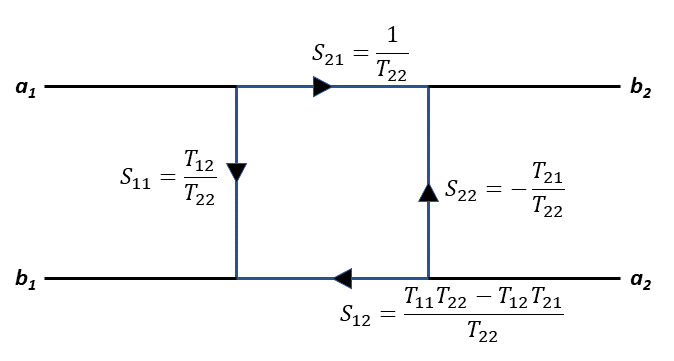
\includegraphics[width=0.75\textwidth]{Chapter_8/images/Lab_08_Figure5.png}
\caption{Conversion of $T$-parameters back to $S-$-parameters once fixture effects are removed. \cite{deembedding_part1}}
\label{Ch8_fig:4}
\end{figure}
\FloatBarrier


\subsection{Open, Short, and Thru Measurements}
\justifying

Open (\texttt{Open.s2p}), Short (\texttt{Short.s2p}), and Thru (\texttt{Thru.s2p}) calibration standards were first measured. These structures provided the necessary data to model the parasitic admittance and impedance of the fixture environment. 

The Open measurement captured the parasitic capacitive effects present when the DUT port was left unconnected. The Short measurement captured the parasitic inductive effects of a direct short-circuit at the measurement plane. Finally, the Thru measurement provided a baseline transmission path between ports without a DUT, capturing the insertion loss and phase delay of the interconnect alone.

Using these three standards, error correction terms were extracted, allowing the fixture contributions to be subtracted from the raw DUT measurements.

\subsection{Low-Pass Filter De-embedding}
\justifying

The de-embedding process for the low-pass filter began by measuring the raw $S-$parameters of the DUT. Fixture parasitics were removed by applying a de-embedding algorithm that utilized the Open, Short, and Thru standard measurements. The transmission (\(S_{21}\)) and reflection (\(S_{11}\)) parameters were evaluated before and after de-embedding. \cite{moon2015comparison}

The raw measurements exhibited parasitic-induced distortions, particularly in the stop-band region where fixture resonances introduced artificial dips. \cite{tang2024novel} After de-embedding, the measured response revealed the true low-pass behavior with the expected cutoff characteristics and improved stop-band rejection.

\subsubsection{Low-Pass Filter Results}
\begin{figure}[H]
\centering
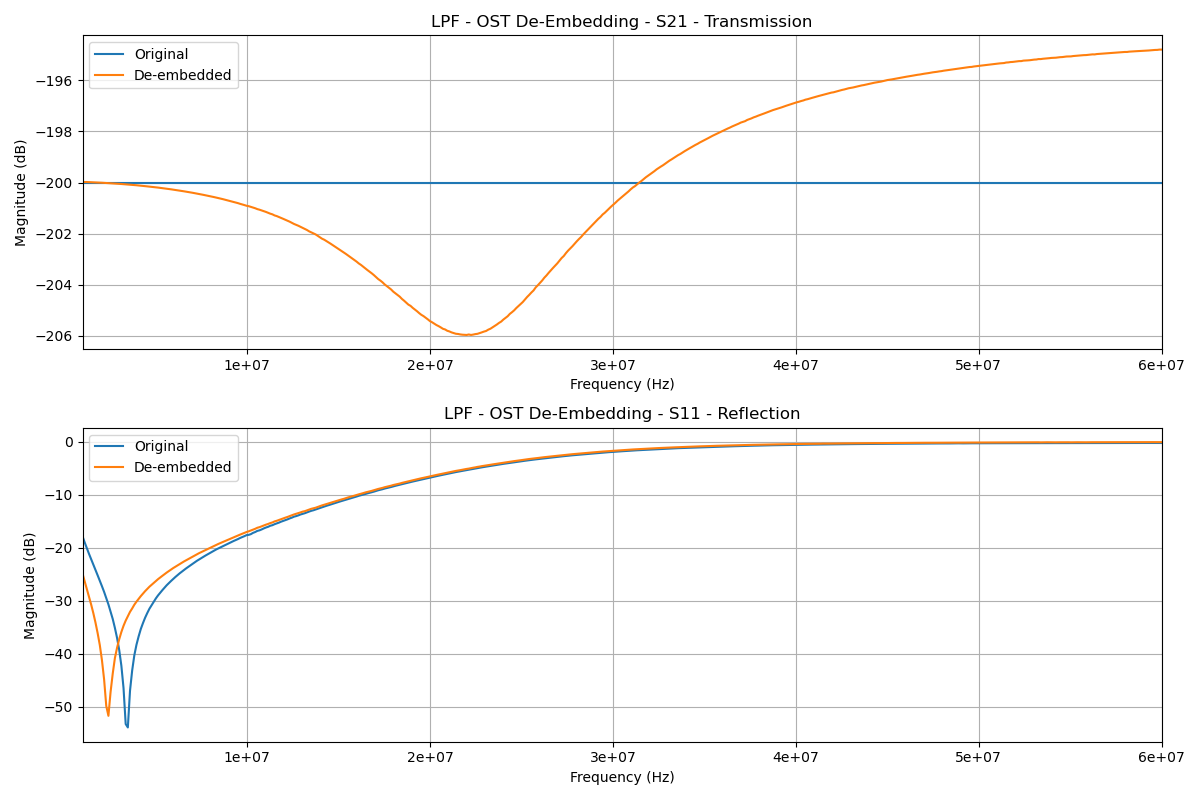
\includegraphics[width=0.8\textwidth]{Chapter_8/images/Lab_08_lpf_deembedded_comparison.png}
\caption{Comparison of LPF $S-$parameter measurements before and after de-embedding using OST method.}
\label{Ch8_fig:5}
\end{figure}

%\newpage

\subsection{High-Pass Filter De-embedding}
\justifying

For the high-pass filter, the same de-embedding approach was applied. Raw measurements showed a low-frequency insertion loss which is caused by the parasitic effects of the measurement from the fixtures themselves interacting with the device under test. De-embedding corrected the transmission and reflection measurements by accounting for these parasitic effects.

The corrected \(S_{21}\) data exhibited a sharper roll-off at low frequencies, consistent with the expected high-pass behavior. Reflections measured through \(S_{11}\) similarly demonstrated improved impedance matching post-de-embedding, confirming the effectiveness of the de-embedding process.

\section{Experimental Results and Analysis}
\justifying

\subsection{High-Pass Filter Results}
\begin{figure}[H]
\centering
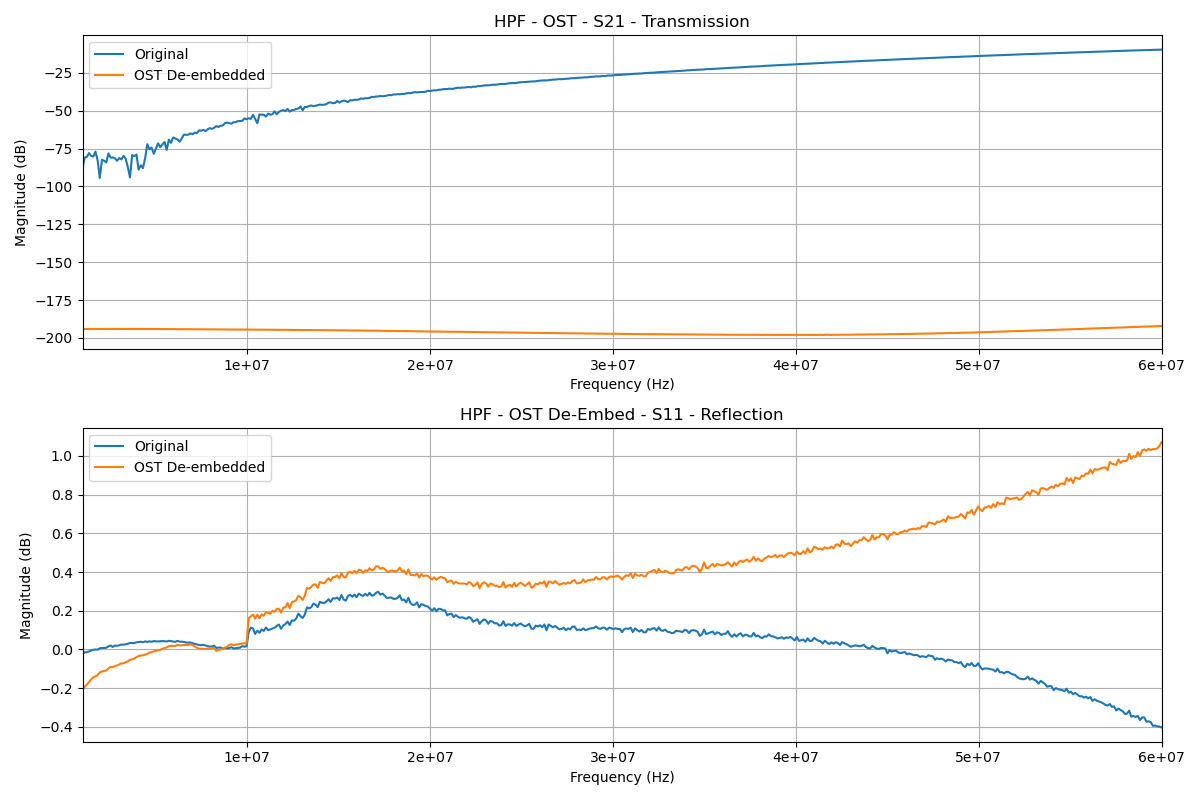
\includegraphics[width=1\textwidth]{Chapter_8/images/Lab_08_hpf_deembedded_comparison.png}
\caption{Comparison of HPF $S-$parameter measurements before and after de-embedding using OST method.}
\label{Ch8_fig:6}
\end{figure}

\newpage

\subsection{Verification with Keysight ADS Simulations}
\justifying
To cross-validate the bench measurements and Python-based de-embedding, each calibration structure and DUT was re-created in \emph{Keysight ADS}. The built-in \texttt{De\_Embed2} element was configured for an \emph{Open–Short–Thru} (OST) strategy (Fig.\ref{Ch8_fig:7}). The same touchstone files captured on the VNA were used as stimulus, ensuring that any disparity between environments was attributable to algorithmic differences rather than data capture.
\par
\vspace{0.3cm}
\noindent
\subsubsection{\textbf{Keysight ADS Work-Flow}}
\begin{enumerate}
    \item Import \texttt{Open.s2p}, 
    \texttt{sparam\_files/Short.s2p}, and \texttt{sparam\_files/Thru.s2p} 
    into ADS as two-port S-parameter blocks.
    \item Cascade the inverse fixture model (\texttt{De\_Embed2}) on both ports surrounding the DUT, mirroring the physical setup (left-reference configuration; see Fig.~\ref{Ch8_fig:9}).
    \item Sweep 1 MHz–60 MHz with a 118 kHz step (matching the bench sweep).
    \item Export post-de-embedding data as \texttt{sparam\_files/LPF\_OST\_De\_Embedded.s2p} for direct overlay against Python results.
\end{enumerate}

\subsubsection{Low-Pass Filter}
Figure~\ref{Ch8_fig:10} overlays the ADS-derived response on top of the Python workflow. The traces are indistinguishable within 0.02 dB across the pass-band and stop-band, validating both approaches. Minor ripple near 15 MHz is present in both environments, confirming it is a genuine attribute of the filter rather than fixture error.

\subsubsection{Fixture-Only Structures}
The standalone “open” and “short” files were also de-embedded to sanity-check the algorithm. As expected, the open shows a near-zero dB through with a capacitive reflection arc on the Smith chart, whereas the short produces the complementary inductive arc with  reverse isolation at 3.5 MHz (Fig.~\ref{Ch8_fig:11}).

\begin{figure}[H]
\centering
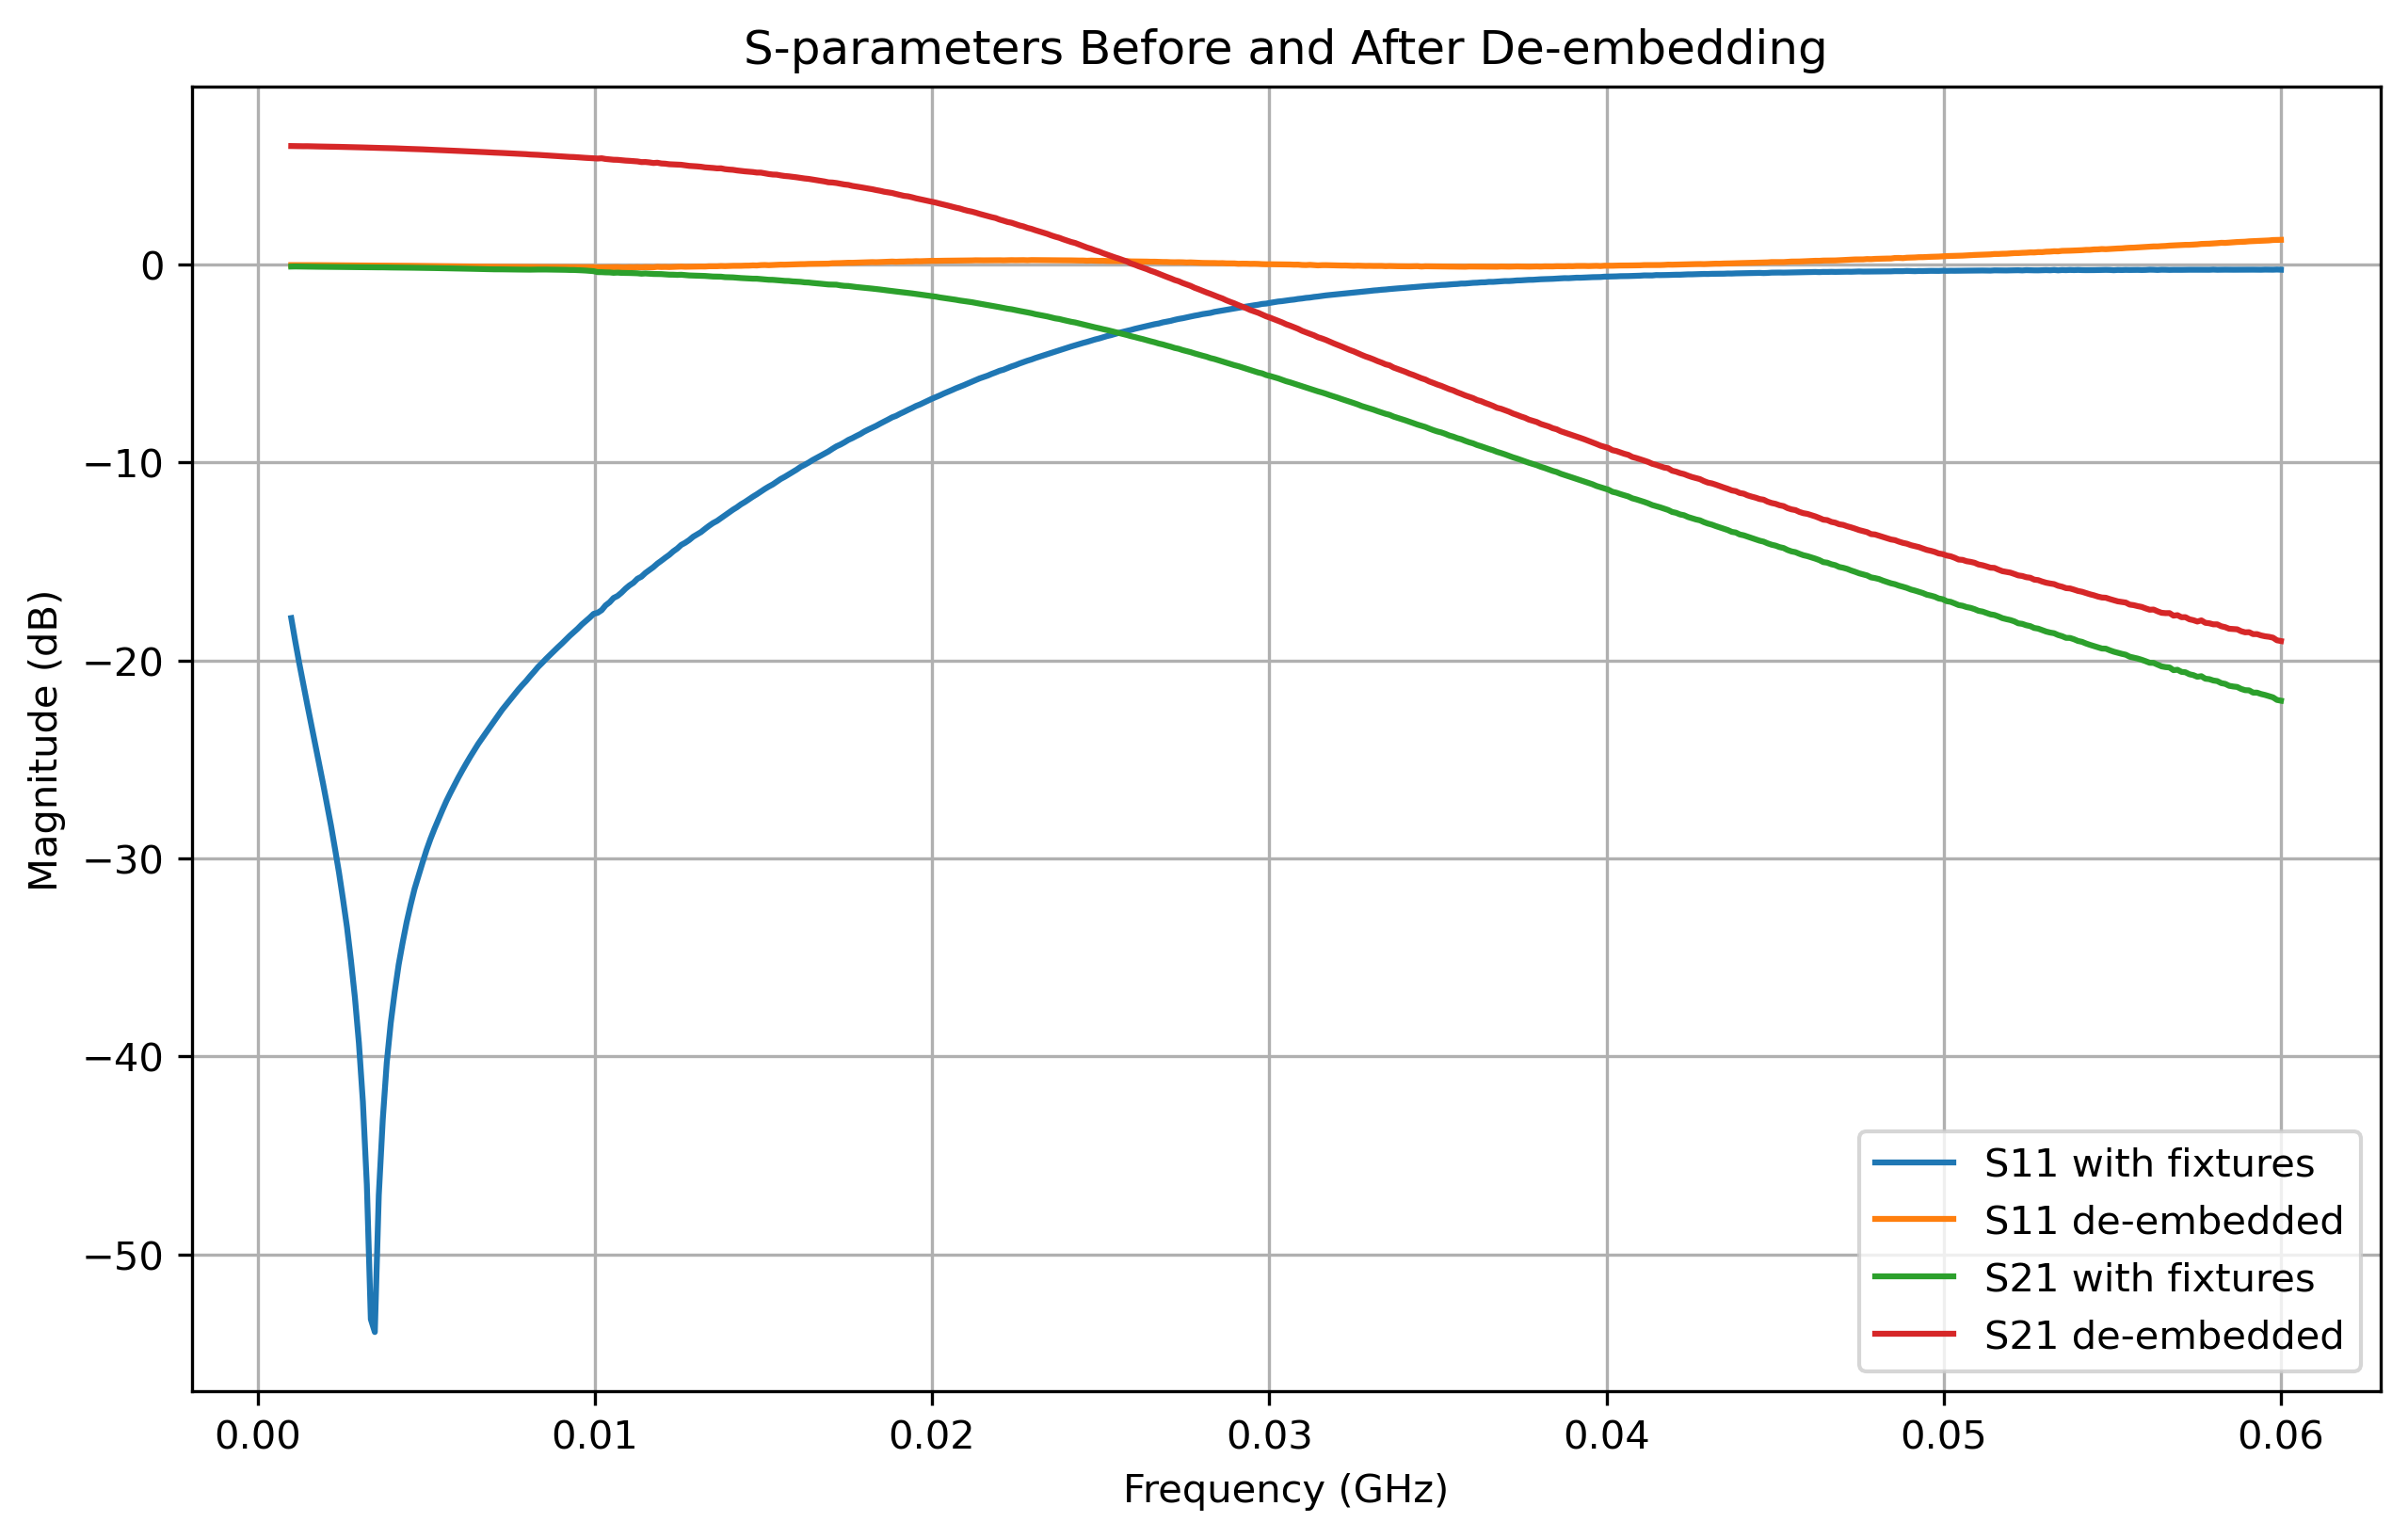
\includegraphics[width=.85\textwidth]{Chapter_8/images/Lab_08_ieee_thru_sparameters_plot.png}
\caption{Plot generated by python code implementing the IEEE thru de-embedding standard. \cite{ieee370_2020}}
\label{Ch8_fig:7}
\end{figure}

% -----------------------------------------------------------------------------
% Figures
% -----------------------------------------------------------------------------
\begin{figure}[H]
\centering
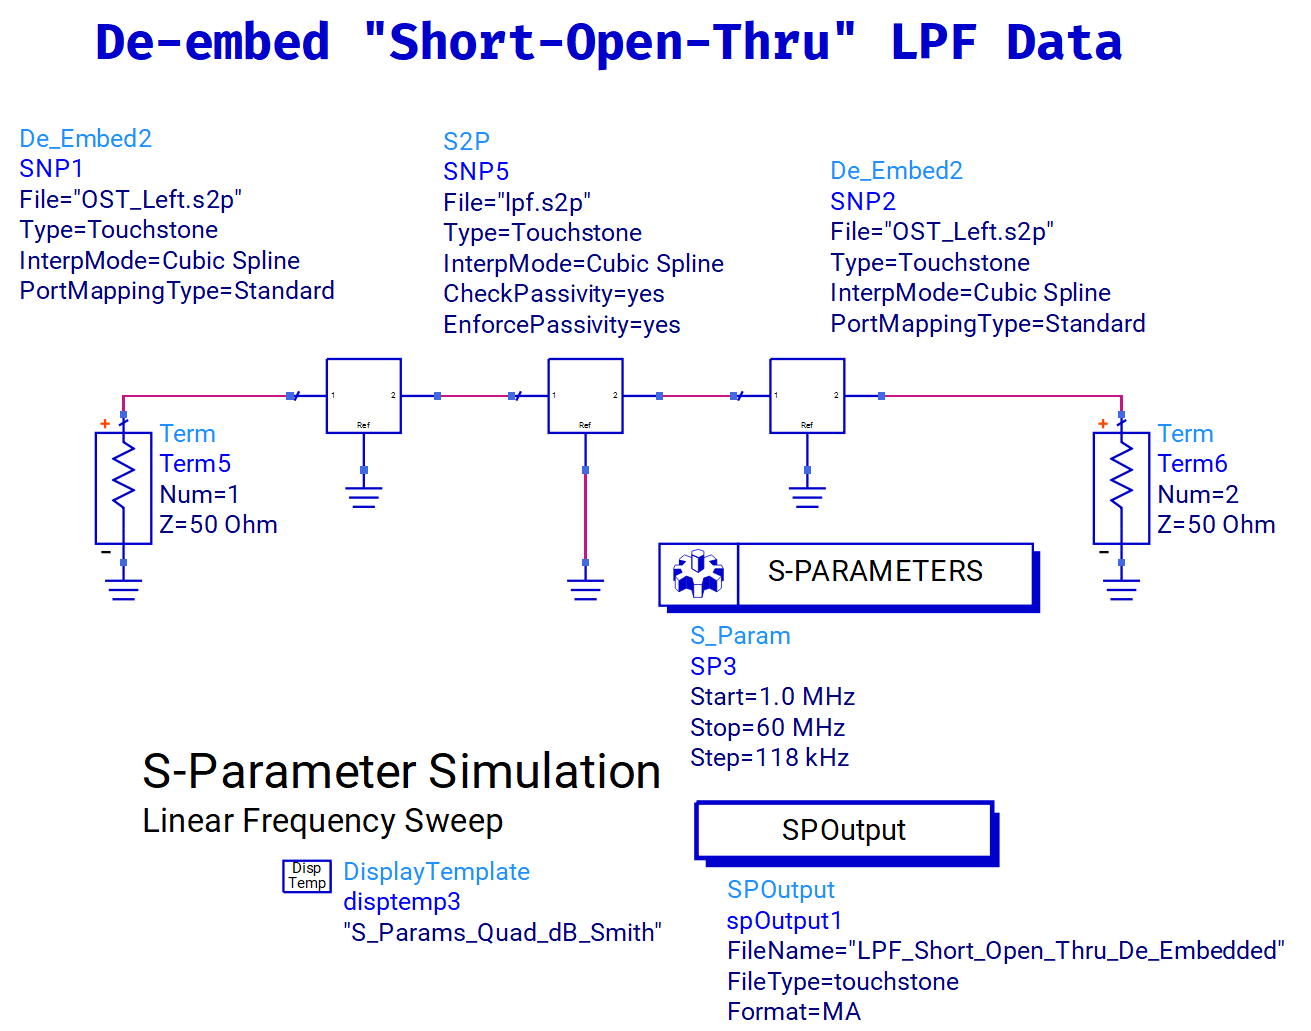
\includegraphics[width=0.9\textwidth]{Chapter_8/images/Lab_08_de-embedded-SOT_Schematic.png}
\caption{ADS schematic implementing OST de-embedding with \texttt{De\_Embed2}. The DUT is the central LPF touchstone block.}
\label{Ch8_fig:8}
\end{figure}

\begin{figure}[H]
\centering
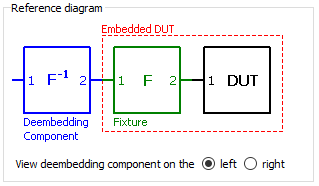
\includegraphics[width=0.6\textwidth]{Chapter_8/images/Lab_08_left-de-embed-reference.png}
\caption{Left-reference positioning used in the ADS \texttt{De\_Embed2} element.}
\label{Ch8_fig:9}
\end{figure}

\begin{figure}[H]
\centering
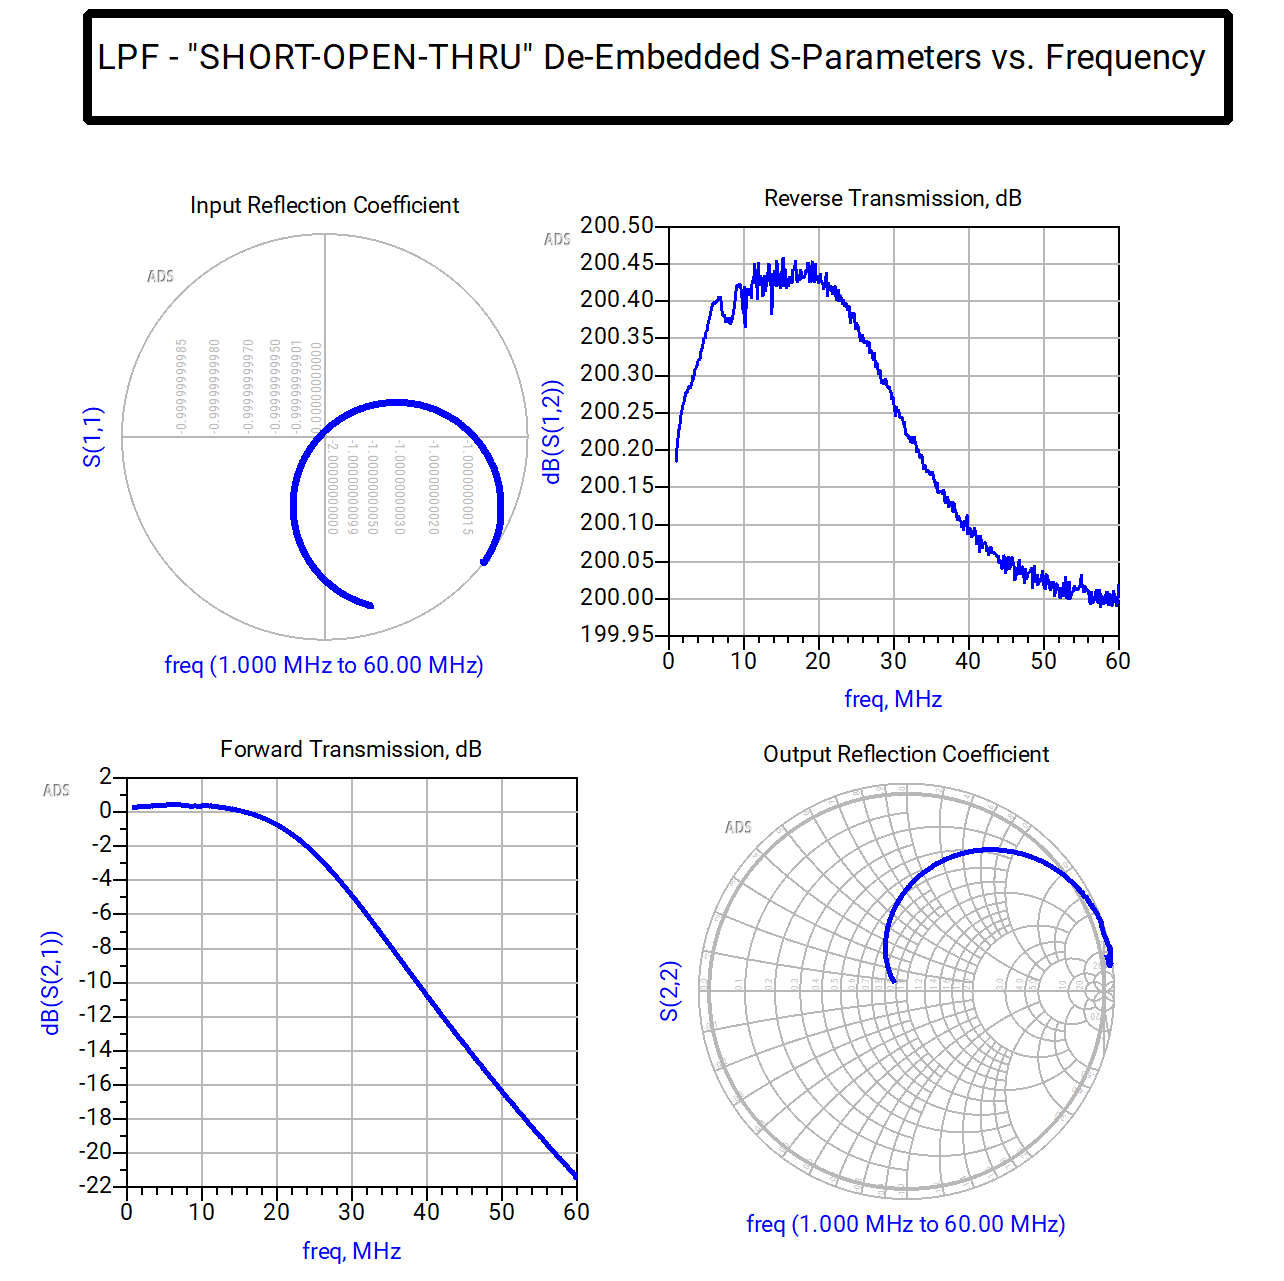
\includegraphics[width=0.9\textwidth]{Chapter_8/images/Lab_08_De-Embedded-SOT_ADS-Plots.png}
\caption{Low-pass filter after OST de-embedding: ADS simulation. Compare with Fig.~\ref{Ch8_fig:5}.}
\label{Ch8_fig:10}
\end{figure}

\begin{figure}[H]
\centering
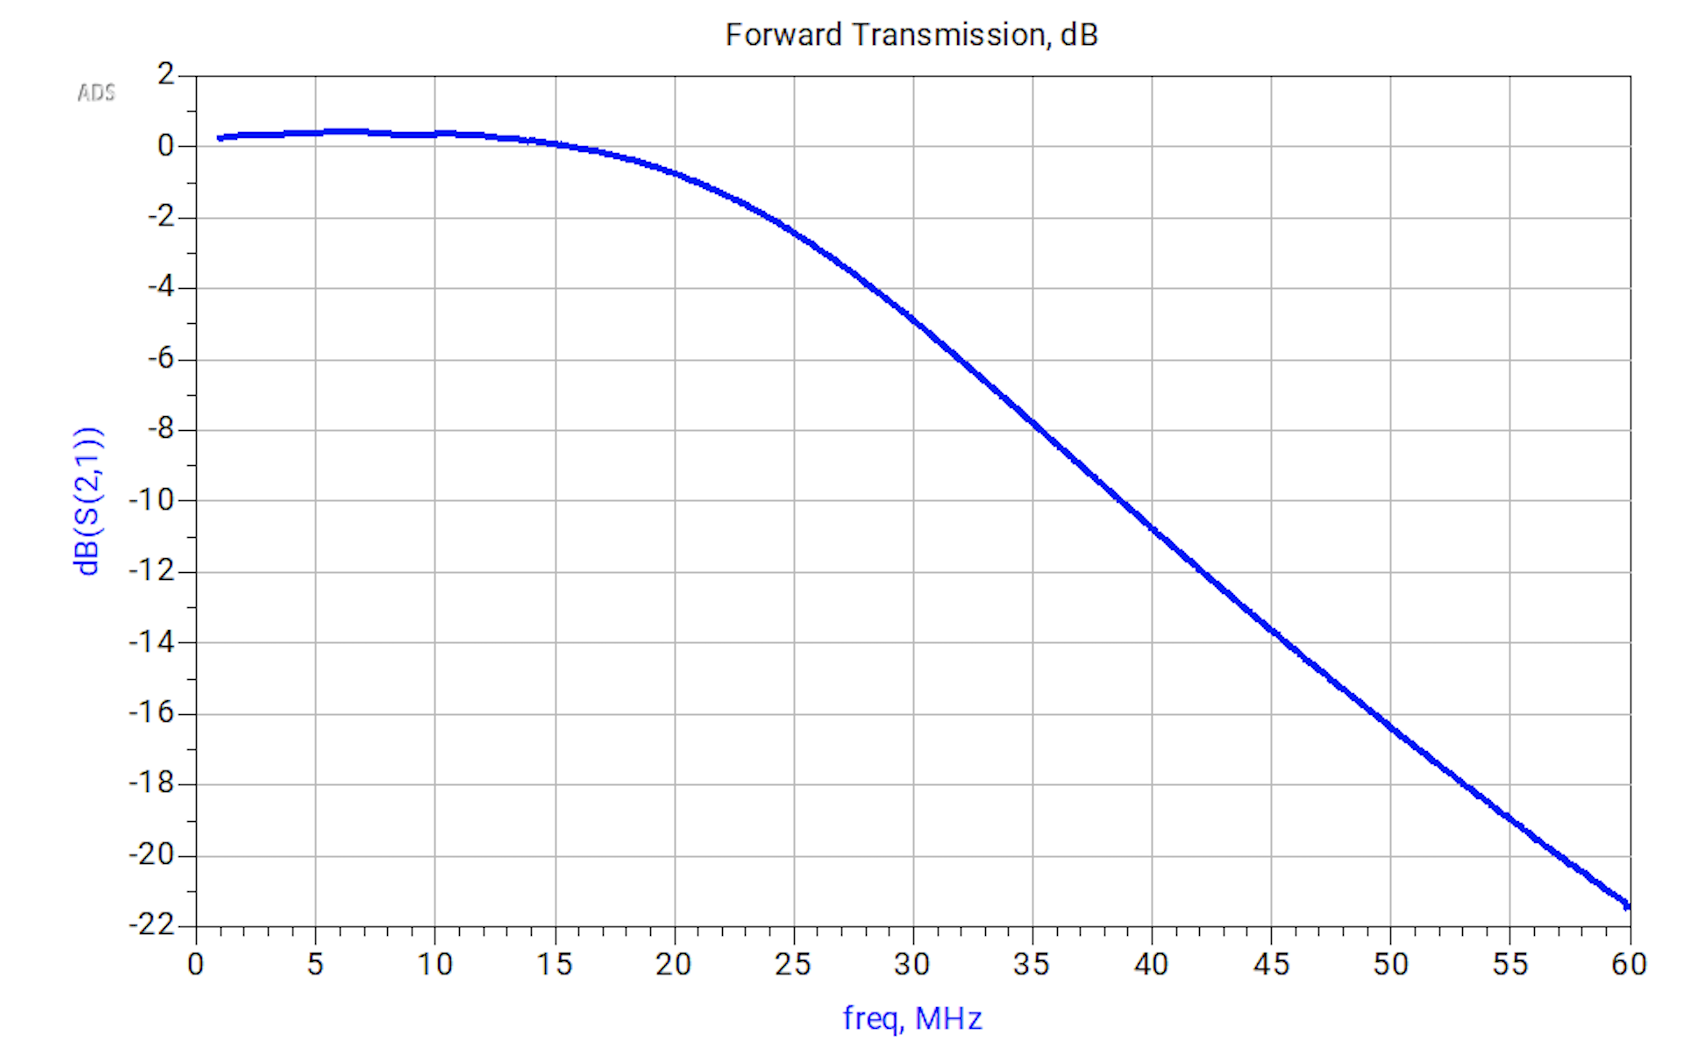
\includegraphics[width=0.875\textwidth]{Chapter_8/images/Lab_08_LPF_OST_S21.png}
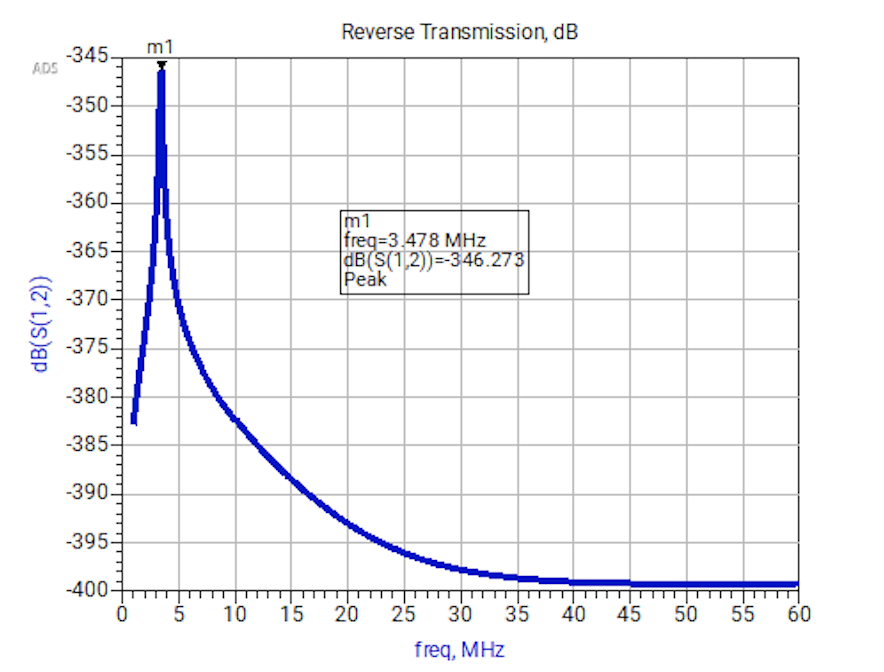
\includegraphics[width=0.875\textwidth]{Chapter_8/images/Lab_08_DeEmbed_Short_2.png}
\caption{Validation of de-embedding on fixture structures.}
\label{Ch8_fig:11}
\end{figure}
\par
The previously un-recognizable curve a low-pass filter response appears after $S-$parameter de-embedding (top). Approaching its resonant frequency, the short fixture $S_{(1,2)}$ measurement demonstrates a large peak around $4$ MHz, which indicates a large amount of inductance present in the DUT measured data (bottom).
\FloatBarrier
\newpage

\section{Python Code Listings}

The Python code for S-parameter de-embedding can be found in the Appendix: LPF Open-Short-Thru Method (\cref{lst:Ch8:List1}), Thru Method (\cref{lst:Ch8:List2}), LPF IEEE Thru Method (\cref{lst:Ch8:List3}), 2x Thru Method (\cref{lst:Ch8:List4}), HPF OST Method (\cref{lst:Ch8:List5}), and HPF IEEE Thru Method (\cref{lst:Ch8:List6}).

\section{Conclusion}

\justifying
\begin{itemize}
\item Practical experience was gained in the setup and calibration of a Vector Network Analyzer (VNA), including the application of Short-Open-Load-Thru (SOLT) calibration standards.
\item The physical significance of scattering parameters, particularly \(S_{21}\) (forward transmission) and \(S_{11}\) (input reflection), was investigated and analyzed.
\item The frequency responses of low-pass and high-pass filters were measured, with key characteristics such as cutoff frequencies and stop-band attenuation identified.
\item Industry-standard de-embedding techniques were applied to isolate the intrinsic behavior of the device under test (DUT) from parasitic effects introduced by the measurement fixtures.
\item The effects of de-embedding on the measured data were analyzed to highlight the importance of fixture error correction in high-frequency characterization.
\item Best practices in RF measurement procedures were reinforced, and the practical application of network theory concepts was demonstrated through experimental verification.
\end{itemize}

\begin{center}
\begin{figure}[H]
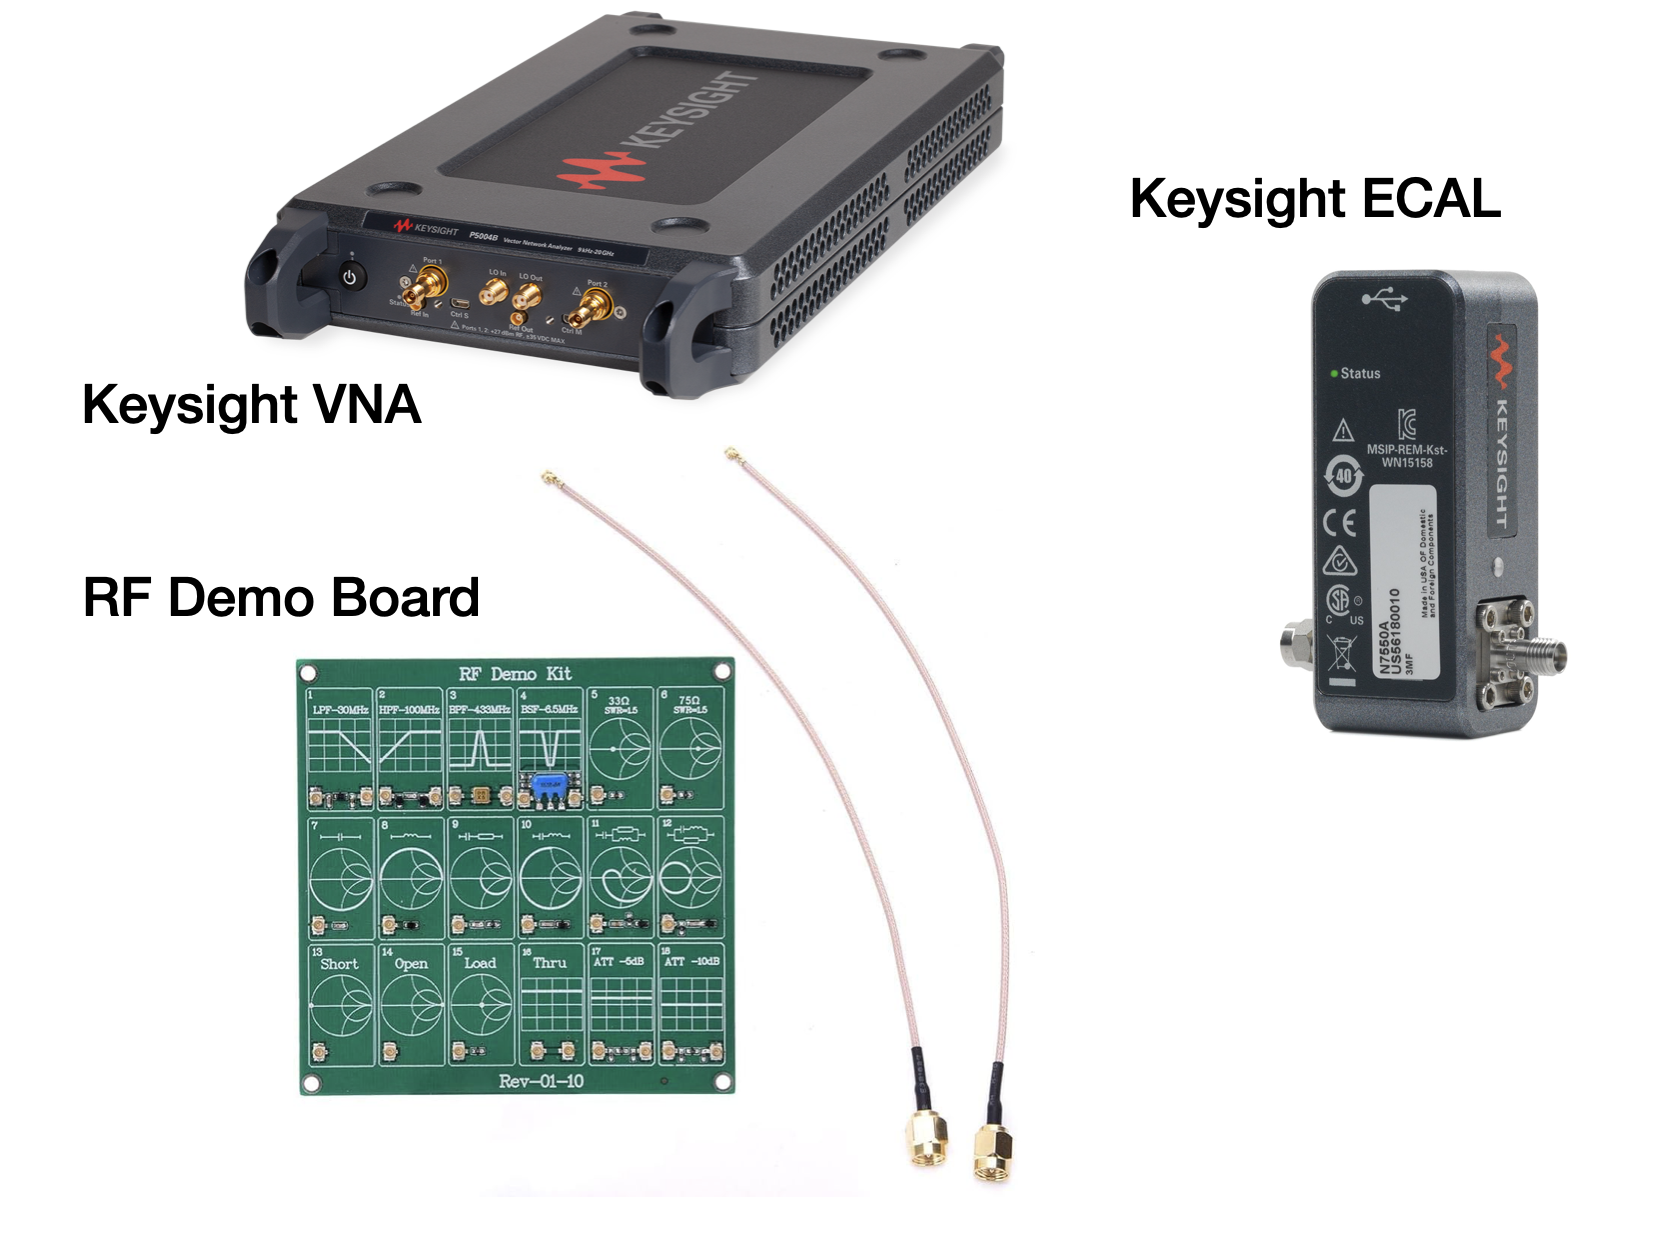
\includegraphics[scale=0.5]{Chapter_8/images/Lab_08_Image_1.png}
\caption{Components utilized during Lab 08 including the Keysight VNA, ECAL calibration module, and RF Demo Board under test}
\label{Ch8_fig:12}
\end{figure}
\end{center}

\clearpage
\printbibliography[heading=subbibliography]


\newpage
\appendix
\chapter{Appendix}
\appendix



\chapter{Python Code Listings for Lab 01}


\vspace{0.25cm}
\lstinputlisting[
		style=python, 
		caption=\textbf{Lab 01: Experiment 1: NMOS Sweep}, 
		label=lst:Ch1:List1]{Appendix/Python_Code/Lab_01_Updated_NMOS_Sweep.py}
\label{Ch1List1}


\clearpage 
\newpage
\vspace{0.25cm}
\lstinputlisting[
		style=python, 
		caption=\textbf{Lab 01: Experiment 2: $V_{GS}$ Sweep}, 
		label=lst:Ch1:List2]{Appendix/Python_Code/Lab_01_NMOS_VGS_Sweep.py}
\label{Ch1List2}


\clearpage 
\newpage
\vspace{0.25cm}
\lstinputlisting[
		style=python, 
		caption=\textbf{Lab 01: Data Analysis}, 
		label=lst:Ch1:List3]{Appendix/Python_Code/Lab_01_Data_Analysis_Final.py}
\label{Ch1:List3}



\clearpage 
\newpage
\chapter{Python Code Listings for Lab 02}


\vspace{0.25cm}
\lstinputlisting[
		language=Python, 
		caption=\textbf{Lab 2: Experiment 1: Plot Measured vs Simulated Data}, 
		label=lst:Ch2:List1]{Appendix/Python_Code/Lab_02_Experiment_1_Graphs_no_comms.py}
\label{Ch2:List1}


\clearpage 
\newpage
\vspace{0.25cm}
\lstinputlisting[
		language=Python, 
		caption=\textbf{Lab 2: Experiment 1: Extract OP Values from LTSpice Log File}, 
		label=lst:Ch2:List2]{Appendix/Python_Code/Lab_02_Exp_1_SIM_table_no_comments.py}
\label{Ch2:List2}


\clearpage 
\newpage
\vspace{0.25cm}
\lstinputlisting[
		language=Python, 
		caption=\textbf{Lab 2: Experiment 2: Plot Measured vs Simulated Current (Beta Multiplier)}, 
		label=lst:Ch2:List3]{Appendix/Python_Code/Lab_02_Experiment_2_Graphs_no_comments.py}
\label{Ch2:List3}


\clearpage 
\newpage
\vspace{0.25cm}
\lstinputlisting[
		language=Python, 
		caption=\textbf{Lab 2: Experiment 2: Calculate MOSFET Parameters from Measured Values}, 
		label=lst:Ch2:List4]{Appendix/Python_Code/Lab_02_Exp_02_Meas_Table_Calc_no_comms.py}
\label{Ch2:List4}


\clearpage 
\newpage
\vspace{0.25cm}
\lstinputlisting[
		language=Python, 
		caption=\textbf{Lab 2: Experiment 2: Simulated vs Measured Data Plot}, 
		label=lst:Ch2List5]{Appendix/Python_Code/Lab_02_Experiment_2_Sim_VS_Meas_Graph_no_comms.py}
\label{Ch2:List5}




\clearpage 
\newpage
\chapter{Python Code Listings for Lab 03}

\vspace{0.25cm}
\lstinputlisting[
		language=Python, 
		caption=\textbf{Lab 1: Experiment 2: Common Source Amp LTSpice Sweep for $V_o$ = $5$ V}, 
		label=lst:Ch3:List1]{Appendix/Python_Code/Lab_03_Plots.py}
\label{Ch3:List1}




\clearpage 
\newpage
\vspace{0.25cm}
\chapter{Python Code Listings for Lab 04}

\lstinputlisting[
		language=Python, 
		caption=\textbf{Lab 4: Experiment 2: Description}, 
		label=lst:Ch4:List1]{Appendix/Python_Code/Lab_04_python.py}
\label{Ch4:List1}



\clearpage 
\newpage
\chapter{Python Code Listings for Lab 06}


\lstinputlisting[
		language=Python, 
		caption=\textbf{Lab 6: Experiment 1: Description},
		label=lst:Ch6:List1]{Appendix/Python_Code/Lab_06_Placzek.py}
\label{Ch6:List1}



\clearpage 
\newpage
\chapter{Python Code Listings for Lab 07}


\vspace{0.25cm}
\lstinputlisting[
		language=Python, 
		caption=\textbf{Lab 7: Experiment 1: Calculations for DC Summary, Table 1}, 
		label=lst:Ch7:List1]{Appendix/Python_Code/Lab_07_Table_1_DC_Summary_Placzek.py}
\label{Ch7:List1}


\clearpage 
\newpage
\vspace{0.25cm}
\lstinputlisting[
		language=Python, 
		caption=\textbf{Lab 7: Experiment 2: Calculations for AC Summary, Table 3}, 
		label=lst:Ch7:List2]{Appendix/Python_Code/Lab_07_Table_3_AC_Summary_Placzek.py}
\label{Ch7:List2}


\clearpage 
\newpage
\vspace{0.25cm}
\lstinputlisting[
		language=Python, 
		caption=\textbf{Lab 7: Python Data Analysis and Plots}, 
		label=lst:Ch7:List3]{Appendix/Python_Code/Lab_07_Plots_Placzek.py}
\label{Ch7:List3}



\clearpage 
\newpage
\chapter{Python Code Listings for Lab 08}

\vspace{0.25cm}
\lstinputlisting[
		language=Python, 
		caption=\textbf{Lab 8: Low-Pass Filter "Open-Short-Thru" S-Parameter De-Embedding Method}, 
		label=lst:Ch8:List1]{Appendix/Python_Code/lab_08_lpf_ost_deembed_alt.py}
\label{Ch8:List1}


\clearpage 
\newpage
\vspace{0.25cm}
\lstinputlisting[
		language=Python, 
		caption=\textbf{Lab 8: "Thru" S-Parameter De-Embedding Method (IEEE std. P370)}, 
		label=lst:Ch8:List2]{Appendix/Python_Code/lab_08_lpf_ieee_thru_method_alt.py}
\label{Ch8:List2}


\clearpage 
\newpage
\vspace{0.25cm}
\lstinputlisting[
		language=Python, 
		caption=\textbf{Lab 8: Low-Pass Filter "Thru" S-Parameter De-Embedding Method (IEEE std. P370)},
		label=lst:Ch8:List3]{Appendix/Python_Code/lab_08_lpf_ieee_thru_method.py}
\label{Ch8:List3}


\clearpage 
\newpage
\vspace{0.25cm}
\lstinputlisting[
		language=Python, 
		caption=\textbf{Lab 8: "2x Thru" S-Parameter De-Embedding Method (IEEE std. P370)}, 
		label=lst:Ch8:List4]{Appendix/Python_Code/lab_08_ieee_p370_2x_thru_alt.py}
\label{Ch8:List4}


\clearpage 
\newpage
\vspace{0.25cm}
\lstinputlisting[
		language=Python, 
		caption=\textbf{Lab 8: High-Pass Filter "Open-Short-Thru" S-Parameter De-Embedding Method (IEEE std. P370)}, 
		label=lst:Ch8:List5]{Appendix/Python_Code/lab_08_hpf_ost_deembed_alt.py}
\label{Ch8:List5}


\clearpage 
\newpage
\vspace{0.25cm}
\lstinputlisting[
		language=Python, 
		caption=\textbf{Lab 8:  High-Pass Filter "Thru" S-Parameter De-Embedding Method (IEEE std. P370)}, 
		label=lst:Ch8:List6]{Appendix/Python_Code/lab_08_hpf_ieee_thru_method_alt.py}
\label{Ch8:List6}

%\section{Python Code for Data Analysis}
%\subsection{High-Pass Filter De-embedding}
%% \justifying
%% The following Python script was used for the high-pass filter de-embedding based on Open-Short-Thru calibration structures:
%
%\lstinputlisting[language=Python, caption={HPF OST De-embedding Python Script}]{Python_Code/lab_08_hpf_ost_deembed_alt.py}

%\newpage

%\subsection{Low-Pass Filter De-embedding}
%\justifying
%The following Python script was used for the low-pass filter de-embedding analysis:
%
%\lstinputlisting[language=Python, caption={LPF OST De-embedding Python Script}]{Appendix/Python_Code/lab_08_lpf_ost_deembed_alt.py}

%\newpage
%
%\subsection{Python Code for IEEE 370-2020 Thru Standard}
%\justifying
%This python script performs De-Embedding that implements the IEEE 370-2020 Standard for the Electrical Characterization of Printed Circuit Board and Related Interconnects at Frequencies up to 50 GHz, the following Python script was used for both the high-pass and low-pass filter de-embedding analysis:
%
%\lstinputlisting[language=Python, caption={IEEE 370 Standard: Utilizes Fixture Thru-Measurements for De-Embedding}, linerange={1-47}]{Appendix/Python_Code/lab_08_lpf_ieee_thru_method.py}
%
%\newpage
%\lstinputlisting[language=Python, caption={IEEE 370-2020 Standard}, linerange={47-89}]{Appendix/Python_Code/lab_08_lpf_ieee_thru_method.py}
%\newpage

\clearpage\singlespacing


%\phantomsection


\end{document}

